\documentclass[11pt,a4paper,twoside,openright,titlepage,
headinclude,footinclude,BCOR=5mm,numbers=noenddot,
cleardoublepage=empty,abstracton,table,usenames,dvipsnames]{scrbook}

\usepackage[T1]{fontenc}
\usepackage[utf8]{inputenc}
\usepackage[english]{babel}
\PassOptionsToPackage{nopatch}{microtype}	% Fix TOC

% Various
\usepackage{lipsum}
\usepackage{url}
\usepackage{quoting}
\usepackage{caption}
\usepackage{subcaption}
\usepackage{comment}
\usepackage{etoc, blindtext}    % Local index
\usepackage[many]{tcolorbox}    % Box
% \tcbuselibrary{theorems}
% \usepackage{enumitem}

% --- STYLE ---
% ArsClassica
\usepackage[eulerchapternumbers,beramono,pdfspacing, parts]{classicthesis}
\usepackage{arsclassica}
\definecolor{lev}{RGB}{50, 38, 216}
\hypersetup{
    linkcolor=lev,      
    urlcolor=lev,
    citecolor=lev
} 

% --- MATHS AND PHYSICS ---
\usepackage[italicdiff]{physics}
\usepackage{siunitx}\sisetup{parse-numbers = false}
\usepackage{amsthm}
% \usepackage{nicematrix}
% \usepackage{tensor}
\usepackage[framemethod=tikz]{mdframed}
\usepackage{mathtools}
\usepackage{amssymb}
\usepackage{bm}

% --- GRAPHICS ---
% Pgfplots
\usepackage{pgfplots}
\pgfplotsset{compat=1.18}
 \pgfplotsset{
    /pgfplots/colormap={levmap}{rgb255=(50,38,216) rgb255=(20,151,249)}
} 
% Fill Between
\usepgfplotslibrary{fillbetween}
\pgfdeclarelayer{ft}
\pgfdeclarelayer{bg}
\pgfsetlayers{bg,ft,main}
% Graphicx
\usepackage{graphicx}
% Tikz and Tikz3D
\usepackage{tikz}
\usepackage{tikz-3dplot}
\usetikzlibrary{decorations.pathmorphing}
\usetikzlibrary{decorations.markings}		% Marks
\usetikzlibrary{arrows.meta} 				% Arrows
% \usetikzlibrary{angles}
\usetikzlibrary{shadings}
\usetikzlibrary{shapes.geometric}
\usetikzlibrary{calc} 						% Perform calculations on positions
\usetikzlibrary{patterns,patterns.meta} 	% Draw patterns
\usepackage[compat=1.1.0]{tikz-feynman}		% Feynman diagrams
%/tikzfeynman/warn luatex=false

% --- BIBLIOGRAPHY AND LICENSE ---
% Bibliography (in TeXstudio: Options/Configure TeXstudio/Build/Default bibliography tool: set "Biber")
\usepackage[autostyle,italian=guillemets]{csquotes}
\usepackage[backend=biber,sorting=none]{biblatex}
% DocLicense
\usepackage[
    type={CC},
    modifier={by-nc-sa},
    version={4.0},
]{doclicense}       % Packages
% --- Ambiente citazione ---

    \newenvironment{cit}[2]
        {
            \begin{mdframed}[
                linewidth=1pt,
                linecolor=lev!50,
                leftmargin=1em,
                bottomline=false,
                topline=false,
                rightline=false,
                innerrightmargin=0pt,
                innertopmargin=0pt,
                innerbottommargin=0pt,
                innerleftmargin=1em,
                skipabove=1em,
                skipbelow=1em
            ]
            \noindent\normalfont   
            \textbf{\citename{#1}{author}}: \textbf{\citetitle{#1}}  (\cite{#1} @ #2)
            \vspace{0.5em}\newline
        }
        {\end{mdframed}}

    
% --- Comandi matematici utili ---
    \def\beq{\begin{equation}}
    \def\eeq{\end{equation}}
    % Numerelli
        \newcommand{\C}{\mathbb{C}}
        \newcommand{\R}{\mathbb{R}}
        \newcommand{\N}{\mathbb{N}}
        \newcommand{\Z}{\mathbb{Z}}
    % Fisica
        \newcommand{\ham}{\hat{H}}
        \newcommand{\hilb}{\mathcal{H}}
        \newcommand{\vphi}{\varphi}
        \newcommand{\normalorder}[1]{\colon #1 \, \colon}
    % Algebra
        % \newcommand{\Id}{\mathbb{1}}[1]{\ensuremath{\mathbf{\bar{#1}}}}
    % Altro
        \newcommand{\nquad}{\mkern-18mu}              % deindentazione
        \newcommand{\sgn}{\mathrm{sgn}}               % funzione segno
        \newcommand{\imp}{\stackrel{!}{=}}            % imposizione
        \newcommand{\questionmarkeq}{\stackrel{?}{=}} % uguale con ?
        \newcommand{\half}{%
          \ifmmode
            \frac{1}{2} % \half in mathmode
          \else
            $1/2$ % \half in text
          \fi
        }
        \newcommand{\ol}[1]{\overline{{#1}}}
        \newcommand{\lrR}[1]{\left({#1}\right)} % left and right round parentheses
        \newcommand{\lrS}[1]{\left[{#1}\right]} % left and right square parentheses
        \newcommand{\lrB}[1]{\left\{{#1}\right\}} % left and right braces
        \newcommand{\dV}[1] {d^3 \mathbf{#1}\,} % elemento di volume        
    % Versors
        \newcommand{\versor}[1]{\ensuremath{\mathbf{\bar{#1}}}}
    
% --- Simbolo per sezioni/sottosezioni Opzionali ---
    \newcommand{\optional}{\texorpdfstring{\textreferencemark{} }{※ }} 

% --- EqBox ---
    % Pacchetto di riferimento: tcolorbox
    \newtcolorbox{eqbox}[1][]{
      colback=lev!15,
      top=0.4em,     
      bottom=0.8em,
      colframe=white,
      width=\textwidth,
      after={\par\smallskip\noindent\ignorespacesafterend}, %
      #1 % parametro (placeholder) per eventuali
         % argomenti facoltativi
    }

% --- Midline arrow
\newcommand{\arrowIn}{
    \tikz \draw[-stealth] (-1pt,0) -- (1pt,0);
}

% --- Indice locale ---
    % Pacchetto di riferimento: etoc
    \newcommand{\chaptertoc}[1][]{%
      \etocsettocstyle{\addsec*{#1}}{}%
      \localtableofcontents%
      \vspace{1cm}
    }    % Definitions


% --- Graphics ---

% Fix Arsclassica TOC
\makeatletter
\renewcommand{\numberline}[1]{% 
  \hb@xt@\@tempdima{\@cftbsnum{#1}\@cftasnum\hfil}\@cftasnumb}
\makeatother

% Numbering within chapter
\numberwithin{equation}{chapter}
\numberwithin{figure}{chapter}

% Footnotes separator
\setlength{\skip\footins}{1cm}

% Version
% \newcommand{\version}{\( 1.0 \)}

% Bibliography
\addbibresource{misc/bibliography.bib}


% --- Compiler ---

\includeonly{
    misc/cover,
    misc/license,
    misc/intro,
    misc/tmp,
    chapters/superconductivity/superconductivity and thermodynamics/superconductivity and thermodynamics,
    chapters/superconductivity/ginzburg-landau theory of superconductivity/ginzburg-landau theory of superconductivity,
    chapters/superconductivity/conventional superconductors/conventional superconductors,
	chapters/superconductivity/cooper pairs how electrons form bound states/cooper pairs how electrons form bound states,
	chapters/superconductivity/the bcs theory/the bcs theory,
	chapters/superconductivity/from bcs to conventional superconductors/from bcs to conventional superconductors
}


\begin{document}
	%    
    \begin{titlepage}

	\raggedleft
	\vspace*{\baselineskip}
	
	\vspace*{0.167\textheight}
	
	%\sffamily %%% CAMBIARE? %%%
    
	\textbf{\spacedallcaps{\Large Notes on}}\\
	[\baselineskip]
	{\textcolor{lev}{\huge \textbf{\spacedallcaps{Superconductivity}}}}

	\vfill
    
    \spacedlowsmallcaps{\Large Alessandro Gori}\\[2ex]
	\rmfamily{Last compiled: \today}
\end{titlepage}
    % Licenza Creative Commons
\newpage
\vspace*{\fill}
\doclicenseThis 
    \include{misc/intro}
	%
    \pdfbookmark{\contentsname}{toc}
    \tableofcontents
	%
    \chapter{superconductivity and thermodynamics}\label{chap:superconductivity and thermodynamics}\chaptertoc{}

Superconductivity is a special state of matter, in which a material exhibits zero resistance and magnetic flux is expelled. It turns out some critical parameters exist, $\mathbf{H}_c$ (critical field) and $T_c$ (critical temperature) separating the normal phase to the superconductive one. Thus, transition to the state of superconductivity is described in the the context of critical phase transition.

Superconductivity involves a wide number of theoretical interesting aspects, from continuous symmetry breaking to condensation of electron pairs, to surprising technological implementations. All in all, it represents an exciting field of physics where thermodynamics, statistical mechanics, quantum mechanics, fluidodynamics and topology collide.

\begin{cit}{tinkham2004introduction}{1.1}
    What Kamerlingh Onnes observed was that the electrical resistance of various metals such as mercury, lead, and tin disappeared completely in a small temperature range at a critical temperature $T_c$, which is characteristic of the material. The complete disappearance of resistance is most sensitively demonstrated by experiments with persistent currents in superconducting rings [...]. Once set up, such currents have been observed to flow without measurable decrease for a year, and a lower bound of some $10^5$ years for theirs characteristic decay time has been established by using nuclear magnetic resonance to detect any slight decrease in the field produced by the circulating current. In fact [...] under many circumstances we expect absolutely no change in field or current to occur in times less than $10^{10^10}$ years!
\end{cit}

This first chapter is devoted to phenomenology. We start by the experimental observations, trying to understand what actually a superconductor \textit{is}. Then we move to the realm of thermodynamics, and study the general phase diagram of ideal superconductors. What presented here is pretty much general and many corrections must be understood in order to describe real superconductors.

\section{Macroscopic theory of superconductivity}

In 1935, the brothers Fritz and Heinz London published their macroscopic theory of superconductivity \cite{london-superconductivity}. The key idea is the following: electrons can be in the normal state (subscript $n$) or in the superconductive one (subscript $s$). Then the density is given by
\[ n = n_n + n_s \]
A critical temperature $T_c$ exists, such that $n_s \neq 0$ if $T \le T_c$. We aim to find some equations to describe the motion of superconducting currents,
\[ \mathbf{J}_s = e n_s \mathbf{v}_s \]
where we consider the electron charge $e=-\abs{e}$ in order to keep the results valid for general charges. Our equations need to exhibit \textbf{perfect conductivity} and \textbf{perfect diamagnetism}. We shall start by the perfect conductivity.

\subsection{The land where electrons do not collide}

Take the Drude theory for the electron motion in crystals,
\[ m \dv{\mathbf{v}}{t} = e \mathbf{E} - \frac{m}{\tau} \mathbf{v} \]
with $m$ the electron mass and $\tau$ the mean scattering time. The superconducting electrons move dissipation-less, meaning $\tau_s \to +\infty$. Then
\[ m e n_s \dv{\mathbf{v}}{t} = e^2 n_s \mathbf{E} \quad\implies\quad \mathbf{E} = \Lambda \pdv{\mathbf{J}_{s}}{t} \qq{with} \Lambda = \frac{m}{e^2 n_s} \]
Obviously this equation describes a free system accelerated by a uniform field. This is the \textbf{first London equation}, describing perfect conductivity.\\

We momentarily drop the subscript $s$, and take for granted the Drude theory of transport (for reference, check \cite{grosso2000solid}); also, every material parameter can be replaced by its effective version in crystals ($m\to m^\star,\varepsilon_0\to\varepsilon^\star$ and so on). By classical electrodynamics, metals are those material capable of perfectly cancel the electric field inside. By the means of Drude theory, dynamic conductivity for large $\tau$ is given by
\[
    \sigma(\omega) = \frac{\sigma_0}{1 - i \omega\tau} \simeq i \frac{\sigma_0}{\omega\tau} \qq{with} \sigma_0 = \frac{ne^2 \tau}{m}
\]
thus perfectly imaginary, $\sigma \simeq i y$ with $y \ge 0$. Then, being the dielectric function related to the conductivity by
\[ 
    \varepsilon(\omega) = 1 + \frac{4\pi i}{\omega}\sigma(\omega) \simeq 1 - \frac{\omega_p^2}{\omega^2} \qq{with} \omega_p^2 = \frac{n e^2}{\varepsilon_0 m} 
\]
we have $\varepsilon(\omega) <0$ for $\omega < \omega_p$. Finally, being the dielectric function related to the complex refraction index by
\[ 
    N^2(\omega) = \varepsilon(\omega) \qq{with} N(\omega) = n(\omega) + i k(\omega)
\]
for $\omega \le \omega_p$ we expect $N \in i \R$, which means the electromagnetic wave is evanescent in the crystal. In first approximation, in dynamic regime, metals are those materials capable of reflecting low-energy waves.\\

We now justify this conclusion. Take Maxwell's equations,
\[
    \begin{aligned}
        \grad \times \mathbf{B} - \frac{1}{c^{2}} \pdv{\mathbf{E}}{t} &= \mu_{0} \mathbf{J} \\
        \grad \times \mathbf{E} &= -\pdv{\mathbf{B}}{t}
    \end{aligned}
\]
By taking the time derivative of the first we get
\[
    \grad \times \lrR{-\pdv{\mathbf{B}}{t}} + \frac{1}{c^{2}} \pdv[2]{\mathbf{E}}{t} = - \mu_{0} \pdv{\mathbf{J}}{t} 
\]
and inserting both the second Maxwell equation and the first London equation, we get
\[
    \grad \times \lrR{ \grad \times \mathbf{E} } + \frac{1}{c^{2}} \pdv[2]{\mathbf{E}}{t} = - \frac{\mu_{0}}{\Lambda} \mathbf{E}
\]
We define $\lambda^2 \equiv \Lambda/\mu_0$, and use the identity 
\[ 
    \grad \times \lrR{ \grad \times \mathbf{A} } = \grad (\grad {\cdot} \mathbf{A}) - \laplacian \mathbf{A} 
\]
then
\begin{equation}
    - \grad \lrR{ \grad \cdot \mathbf{E} } + \laplacian \mathbf{E}  - \frac{1}{c^2} \pdv[2]{\mathbf{E}}{t} = \frac{\mathbf{E}}{\lambda^2}
\end{equation}
Now, consider a purely transversal wave, $\mathbf{E}(\mathbf{x},t) = E_z (x,t) \versor{z}$. Then, Fourier-transforming in frequency domain, we get
\[
    \pdv[2]{}{x} E_{z}(x, \omega) - \lrR{ \frac{1}{\lambda^{2}}-\frac{\omega^{2}}{c^{2}} } E_{z}(x, \omega)=0
\]
the solution to the above equation is a wave
\[
    E_z (x, \omega) = e^{-x / \ell(\omega)} E_z(0,\omega)
    \qq{with}
    \frac{1}{\ell^2(\omega)} \equiv \frac{1}{\lambda^2} - \frac{\omega^2}{c^2}
\]
If
\[
    \frac{1}{\lambda} - \frac{\omega}{c} > 0
    \quad\implies\quad
    \omega < \frac{c}{\lambda} = \sqrt{\frac{\mu_0}{\Lambda}} c = \sqrt{\frac{n e^2}{m \varepsilon_0}} = \omega_p
\]
then $\ell(\omega) \in \R$, meaning the wave is evanescent and suppressed on a length scale $\ell(\omega)$, as expected. This makes sense because the ability of exciting plasmonic modes is independent of the presence of dissipation modes. For $\omega \le \omega_p$, we shall approximate $\ell(\omega) \simeq \lambda$: thus $\lambda$ is the characteristic length scale over which a static field penetrates the superconductor (\textbf{penetration length}):
\[
    \lambda^2 = \frac{m}{\mu_0 e^2 n_s}
\]
Evidently, for vanishing superconducting densities $n_s \to 0$, $\lambda$ is divergent. \\

What about magnetic fields? The same procedure yields
\[
    \lrS{ \nabla^{2} - \frac{1}{c^2} \pdv[2]{}{t} - \frac{1}{\lambda^{2}} } \pdv{\mathbf{B}}{t} = 0 
    \quad\Rightarrow\quad
    \lrS{ \nabla^{2} -  \lrR { \frac{1}{\lambda^2} - \frac{\omega}{c^2} } } (-i\omega) \mathbf{B} (\omega) = 0
\]
The same limit, $\omega\to 0$, now poses a difference: any magnetic flux density $\mathbf{B}$ (we shall call it that way not to confuse it with the external magnetic field $\mathbf{H}$) now solves this equation. Then, \textbf{a perfect conductor perfectly cancels any static electric field and traps any static magnetic flux density}. Also, perfect conductors do not exist.

\begin{figure}
    \centering
    \begin{tikzpicture}
    \begin{axis}[
        axis x line=center,
        axis y line=center,
        axis on top,
        xlabel={$T$},
        ylabel={$H$},
        xlabel style={below right},
        ylabel style={above left},
        xtick={0.33,0.6},
        ytick={1.2},
        xticklabels={$T_c$,$T_0$},
        yticklabel={$H_0$},
        xmin=-0.15,
        xmax=0.8,
        ymin=-0.25,
        ymax=1.75]

        \fill[color=lev!30,opacity=0.5] (0,0) rectangle (0.33,1.7);

        % Path 1
        \draw[color=lev,dashed] (0.6,1.2) -- (0.25,1.2) node[
        	sloped,
        	pos=0.5,
        	allow upside down
        ]{\arrowIn};
        \draw[color=lev,dashed] (0.25,1.2) -- (0.25,0) node[
        	sloped,
        	pos=0.5,
        	allow upside down
        ]{\arrowIn};

        % Path 2
        \draw[color=lev] (0.6,1.2) -- (0.6,0) node[
        	sloped,
        	pos=0.5,
        	allow upside down
        ]{\arrowIn};
        \draw[color=lev] (0.6,0) -- (0.25,0) node[
        	sloped,
        	pos=0.5,
        	allow upside down
        ]{\arrowIn};

        \filldraw[color=lev] (0.6,1.2) circle (2pt) node[anchor=south]{\scriptsize Starting state};
        \filldraw[color=lev] (0.25,0) circle (2pt) node[anchor=north east]{\scriptsize Final state};

        \node (phase) at (axis cs:0.165,1.4) [align=center,color=lev!60]{\tiny Superconducting\\[-1ex] \tiny phase};    
    \end{axis};
\end{tikzpicture}
    \caption{The sketch of the two processes described in text. The starting state is at temperature $T_0$ and the applied magnetic field is $H_0$. The final state is at temperature below the critical temperature and at zero applied field. In this simple context we are neglecting the fact that for high fields the system escapes the superconducting region.}
    \label{fig:perfect conductors and thermodynamics}
\end{figure}

The reason is of thermodynamic stability. Consider the a system at temperature $T_0 > T_c$, under the influence of an external field $H_0$, as sketched in Fig.~\ref{fig:perfect conductors and thermodynamics}. Suppose we work at suitably low fields to neglect the $H$ dependence of the superconducting region (as it will turn out, such a region will exhibit a critical boundary $H_c(T)$). Suppose, also, to change the parameters adiabatically: at any given instant $H$ (and thus $B$) is static. If we follow the solid path, entering the superconducting region at $H=0$: then we expect the final state to show $B=0$. If, instead, we follow the dashed path, we enter the superconducting region at $H\neq 0$; then the magnetic flux density $B\neq 0$ is trapped in the following. Then the final state is ill-defined, being its thermodynamic quantities ambivalent. It follows that a perfect conductor is \textbf{not} a stable state, thus it doesn't exist.

\subsection{The land where magnetic fields are not welcome}

Evidently, our first attempt to describe superconductivity needs some refinement, and superconductors are something more than very good conductors.

\begin{cit}{tinkham2004introduction}{1.1}
    Thus, \textit{perfect conductivity} is the first traditional hallmark of superconductivity. It is also the prerequisite for the most potential applications, such as high current transmission lines or high-field magnets.

    The next hallmark to be discovered was \textit{perfect diamagnetism}, found in 1933 by Meissner and Ochsenfeld. They found that not only a magnetic field is \textit{excluded} from entering a superconductor [...], as might appear to be explained by perfect conductivity, but also that a field in an originally normal sample is \textit{expelled} as it is cooled through $T_c$. This certainly could \textit{not} be explained by perfect conductivity, which would tend to trap the flux \textit{in}.
\end{cit}

We take the curl of the first London equation using Faraday's law
\[
    \grad\times\mathbf{E} = \grad\times \Lambda \pdv{{\mathbf{J}}_s}{t}
    \quad\implies\quad
    \grad \times \Lambda \pdv{\mathbf{J
    }_s}{t} + \pdv{\mathbf{B}}{t} = 0 
\]
Then we postulate this equation holds without the time derivative, from a purely phenomenological perspective. Thus, we got the \textbf{London equations}
\begin{eqbox}
    \vspace{-0.4em}
    \begin{align}
        \mathbf{E} &= \Lambda \dot{\mathbf{J}}_s \label{eq:London1} \\
        \mathbf{B} &= \grad\times\lrR{-\Lambda\mathbf{J}_s} \label{eq:London2}
    \end{align}
\end{eqbox}
Notice that the second one, at this stage, is not well-justified. Evidently, it is equivalent to the equation
\[ 
    \mathbf{A}_s (\mathbf{x},t) = - \Lambda \mathbf{J}_s (\mathbf{x},t) + \grad F(\mathbf{x},t)
\]
with $\mathbf{A}_s$ the electromagnetic vector potential and $F$ some scalar function. Now we can impose physical constraints, to fix the gauge. First, the supercurrent must be zero in the bulk and only flow on the sample boundary $\partial\Omega$. Also, we impose such a boundary supercurrent to flow parallel to the surface $\partial\Omega$ (a perpendicular component would imply charge cumulating on the superconductor surface). Finally, we impose no superconductive charge to cumulate inside the bulk. These conditions read
\begin{equation}\label{eq:LondonGaugeCurrentConditions}
    \grad\cdot\mathbf{J}_s = 0
    \qquad
    \mathbf{J}_s(\mathbf{x},t) \big|_{\mathbf{x}\not\in\partial\Omega} = 0
    \qquad
    \mathbf{J}_s(\mathbf{x},t) \big|_{\mathbf{x}\in\partial\Omega} \perp \partial\Omega \versor{n}
\end{equation}
with $\versor{n}$ the surface element versor. Those conditions ensure \textbf{perfect diamagnetism}, thanks to the second London equation \eqref{eq:London2}. In fact, from Maxwell's equation for static fields
\[
    \grad\times\mathbf{B} = \mu_0 \mathbf{J}_s
    \;\Rightarrow\;
    -\laplacian\mathbf{B} = -\frac{\mu_0}{\Lambda} \grad\times\lrR{-\Lambda\mathbf{J}_s}
    \;\Rightarrow\;
    \lrS{\laplacian - \frac{1}{\lambda^2}}\mathbf{B}=0
\]
which is solved by an exponentially suppressed field,
\[
    \mathbf{B}(\mathbf{x}) = e^{-\abs{\mathbf{x}}/\lambda} \mathbf{B(\mathbf{0})}
\]
We can impose the same conditions as Eq.~\eqref{eq:LondonGaugeCurrentConditions} on the vector potential,
\begin{equation}\label{eq:LondonGauge}
    \grad\cdot\mathbf{A}_s = 0
    \qquad
    \mathbf{A}_s(\mathbf{x},t) \big|_{\mathbf{x}\not\in\partial\Omega} = 0
    \qquad
    \mathbf{A}_s(\mathbf{x},t) \big|_{\mathbf{x}\in\partial\Omega} \perp \partial\Omega \versor{n}
\end{equation}
thus defining the so-called \textbf{London gauge}. In this gauge we completely identify the vector potential and the superconducting current up to a factor $-\Lambda$. Notice that, in this gauge
\[
    - \pdv{\mathbf{A}_s}{t} = \Lambda \pdv{\mathbf{J}_s}{t} = \mathbf{E}
\]
which is the correct potential equation for the electric field, provided a null electric potential gradient. Then Eq.~\eqref{eq:London1} and Eq.~\eqref{eq:London2} can be summarized in
\begin{equation}\label{eq:LondonPotential}
    \mathbf{A}_s = - \Lambda \mathbf{J}_s
\end{equation}
which is coherent because gauge was fixed. London's gauge, essentially, expresses the conservation of the particles number.

\section{Thermodynamics}
We shall now concentrate on some thermodynamic aspects of the theory. In the absence of electromagnetic contributions, the free energy is given by
\[
    F \equiv E - TS
\]
In order to include the electromagnetic contributions over a volume $\Omega$, we need to correct its infinitesimal part by
\[
    dF_m \equiv dF + \mu_0 \int_{\Omega} d^D \mathbf{r} \, \mathbf{H} \cdot d\mathbf{M}
\]
Suppose now no field is applied. Thus we may drop the subscript $m$, being the free energy non magnetic. We indicate with the superscript $(\mathrm{n})$ the normal state and with $(\mathrm{s})$ the superconducting state. The \textbf{condensation energy} $\Delta f$ is given by
\[
    \Delta f (T) = f^{(\mathrm{n})}(T) - f^{(\mathrm{s})}(T)
\]
Evidently, if $\Delta f_m > 0$, the superconducting phase is favorite. Pay attention to the fact that we are at zero magnetic field.

\subsection{The critical field}\label{sec:the critical field}

$F_m$, the \textbf{magnetic free energy}, has the magnetization as its natural variable. We prefer to work with $\mathbf{H}$ as a natural variable, therefore we define the \textbf{magnetic Gibbs free energy} as its Legendre transform
\[
    G_m = F_m - \mu_0 \int_{\Omega} d^D \mathbf{r} \, \mathbf{H} \cdot \mathbf{M}
    \quad\implies\quad
    dG_m = dF - \mu_0 \int_{\Omega} d^D \mathbf{r} \, \mathbf{M} \cdot d\mathbf{H}
\]
We define the energy densities per unit volume
\[
    f = \frac{F}{\Omega}
    \qquad\qquad
    g_m = \frac{G_m}{\Omega}
\]
Thus at some fixed temperature $T$
\[
    g_m (T,\mathbf{H}) = \int_{(T,\,\mathbf{0})}^{(T,\,\mathbf{H})} dg_m (T,\mathbf{H}') = f(T) - \mu_0 \int_{(T,\,\mathbf{0})}^{(T,\,\mathbf{H})} d\mathbf{H}' \cdot \ev{\mathbf{M}(\mathbf{H}')}
\]
where
\[
    \ev{\mathbf{M}} = \frac{1}{\Omega} \int_\Omega d^D \mathbf{r} \, \mathbf{M}
\]
Let us comment briefly the above equations. The integrals are intended as adiabatic along the path connecting the states $(T,\mathbf{0})$ to $(T,\mathbf{H})$. We start from a zero applied field because $g_m$ is to be interpreted as the free energy for establishing a $\mathbf{H}$ field starting from a rest condition. The physical picture could be one of a solenoid embedding a superconductor, with a slowly varying current applying a locally static field $\mathbf{H}'$. Notice that the free enegy part, $f$, is non-magnetic and thus depends only on the temperature.

\begin{figure}
    \centering
    \begin{tikzpicture}
    \begin{axis}[
        axis x line=center,
        axis y line=center,
        axis on top,
        xlabel={$T$},
        ylabel={$H$},
        xlabel style={below right},
        ylabel style={above left},
        xtick={0.5},
        ytick={1},
        xticklabel={$T_c$},
        yticklabel={$H_c(0)$},
        xmin=-0.2,
        xmax=0.8,
        ymin=-0.2,
        ymax=1.2]

        \addplot[draw=none,fill=lev!30,opacity=0.5,domain=0:0.5] {1 - 4*x^2} |- (0,0) -- (0,1);
        \addplot[color=lev,domain=0:0.5] {1 - 4*x^2};

        \node (phase) at (axis cs:0.18,0.4) [align=center,color=lev!60]{\tiny Superconducting\\[-1ex] \tiny phase};
        \node (curve) at (axis cs:0.2,0.8) [anchor=south west,color=lev]{$H_c(T)$};
    \end{axis}
\end{tikzpicture}
    \caption{Sketch of the general critical field dependence on temperature, as depicted in the text.}
    \label{fig:critical region}
\end{figure}

Inside a superconductor all the magnetic flux density, $\mathbf{B}$, is expelled. Thus we have $\mathbf{M} = \ev{\mathbf{M}} = - \mathbf{H}$. Substituting this result in the equation for $g_m$ we get
\begin{equation}\label{eq:critical field preliminary}
    g_m^{(\mathrm{s})}(T,\mathbf{H}) = f^{(\mathrm{s})}(T) + \mu_0 \int_{(T,\,\mathbf{0})}^{(T,\,\mathbf{H})} d \mathbf{H}' \cdot \mathbf{H}' = f^{(\mathrm{s})}(T) + \frac{\mu_0 H^2}{2} \bigg|_{@T}
\end{equation}
We expect a critical field $\mathbf{H}_c(T)$ to exist: it is unphysical to think that any material could expel an arbitrarily large applied magnetic field. This is proved by experiments. Then, we understand that the phase transition occurs whenever
\[
    g_m^{(\mathrm{s})}(T,\mathbf{H}) = g_m^{(\mathrm{n})}(T,\mathbf{H})
\]
We can neglect the magnetic contribution to $g_m^{(\mathrm{n})}$, considering non-magnetic materials. Then we define the \textbf{critical field} $H_c(T)$ as
\begin{eqbox}
    \begin{equation}\label{eq:critical field}
        H_c^2(T) = \frac{2}{\mu_0} \Delta f(T)
    \end{equation}
\end{eqbox}
delimiting a superconducting region. Experimentally it turns out
\[
    H_c(T) \simeq H_c (0) \lrR{1 - \frac{T^2}{T_c^2}}
\]
as plotted in Fig.~\ref{fig:critical region}.

In the following, we will always use the variable $H$ instead of $\mathbf{H}$, assuming isotropy and therefore dependence only on the field intensity. We now make use of thermodynamics to analyze the order of the phase transition in the two cases $H\neq0$ and $H=0$.

\subsection{First order transition at non-zero field}\label{sec:first order transition}

\begin{figure}
    \centering
    \begin{tikzpicture}
    \begin{axis}[
        axis x line=center,
        axis y line=center,
        axis on top,
        xlabel={$T$},
        ylabel={$H$},
        xlabel style={below right},
        ylabel style={above left},
        xtick={0.418,0.5},
        ytick={0.3,1},
        xticklabels={$T_c^\star$,$T_c$},
        yticklabels={$H_0$,$H_c(0)$},
        xmin=-0.2,
        xmax=0.8,
        ymin=-0.2,
        ymax=1.2]

        \addplot[draw=none,fill=lev!30,opacity=0.5,domain=0:0.5] {1 - 4*x^2} |- (0,0) -- (0,1);
        \addplot[color=lev,domain=0:0.5] {1 - 4*x^2};
        \draw[color=black] (0.15,0.3) -- (0.6,0.3) node[
        	sloped,
        	pos=0.5,
        	allow upside down
        ]{\arrowIn};
        \draw[dashed,color=gray!60] (0.418,0) -- (0.418,0.3);
        \draw[dashed,color=gray!60] (0,0.3) -- (0.15,0.3);
        \filldraw[color=black] (0.15,0.3) circle (1.2pt) node {};
        \filldraw[color=black] (0.6,0.3) circle (1.2pt) node {};
    \end{axis}
\end{tikzpicture}
    \caption{The phase transition described in Sec.~\ref{sec:first order transition}. $H_0$ is the uniform applied field, kept constant and non-zero. Phase transition occurs at temperature $T_c^\star < T_c$.}
    \label{fig:critical region first order}
\end{figure}

First, we consider the transition at finite applied field $H_0 \neq 0$, varying the temperature $T$ as sketched in Fig.~\ref{fig:critical region first order}. We may look at entropy per unit volume, defined as
\[
    s(T,H_0) \equiv \frac{S(T,H_0)}{\Omega} = -\lrS{ \pdv{}{T} g_{m}(T, H) }_{H = H_0}
\]
Notice that, due to Eq.~\eqref{eq:critical field preliminary},
\[
\begin{aligned}
    g_m^{(\mathrm{s})} (T,H) - g_m^{(\mathrm{s})} (T,0) &= \lrS{ g_m^{(\mathrm{n})} (T,H) + \Delta f(T) + \frac{\mu_0 H^2}{2} }\\
    &\hspace{7.5em}- \lrS{ g_m^{(\mathrm{n})} (T,0) + \Delta f(T) } \\
    &= \lrS{ g_m^{(\mathrm{n})} (T,H) - g_m^{(\mathrm{n})} (T,0) } + \frac{\mu_0 H^2}{2} = \frac{\mu_0 H^2}{2}
\end{aligned}
\]
where in the last passage we used that the normal state is non-magnetic, therefore its free energy is independent of the field applied. It follows
\[
    g_m^{(\mathrm{s})} (T,H) = g_m^{(\mathrm{s})} (T,0) + \frac{\mu_0 H^2}{2}
\]
From Eq.~\eqref{eq:critical field preliminary} it follows
\[
    g_m^{(\mathrm{s})}(T,0) = g_m^{(\mathrm{s})}(T,H_c(T)) - \frac{\mu_0 H_c^2(T)}{2}
\]
since both sides are equal to $f^{(\mathrm{s})}(T)$, unvaried by the presence of the field. Moreover, $g_m^{(\mathrm{s})}(T,H_c(T)) = g_m^{(\mathrm{n})}(T,H_c(T))$ by the definition of the critical field, Eq.~\eqref{eq:critical field}. Then
\[
\begin{aligned}
    g_m^{(\mathrm{s})} (T,H) &= g_m^{(\mathrm{n})} (T,H_c(T)) + \frac{\mu_0}{2} \lrS{ H^2 - H_c^2(T) } \\
    &= g_m^{(\mathrm{n})} (T,H) + \frac{\mu_0}{2} \lrS{ H^2 - H_c^2(T) }
\end{aligned}
\]
being, once again, the normal state Gibbs energy independent of the field. Then the entropy difference in following the path in Fig.~\ref{fig:critical region first order} is a function of temperature
\[
\begin{aligned}
    \Delta s(T,H_0) &= s^{(\mathrm{n})}(T,H_0) - s^{(\mathrm{s})}(T,H_0) \\
                    &= -\lrS{ \pdv{}{T} g_m^{(\mathrm{n})}(T, H) - \pdv{}{T} g_m^{(\mathrm{s})}(T, H) }_{H = H_0} \\
                    &= \frac{\mu_0}{2} \pdv{}{T} \lrS{ H_c^2(T) - H_0^2 }\\
                    &= \mu_0 H_c(T) \pdv{}{T} H_c(T)\\
                    &\simeq \mu_0 H_c^2 (0) \lrR{1 - \frac{T^2}{T_c^2}} \lrR{ - \frac{2T}{T_c^2} } \qq{for} T < T_c
\end{aligned}
\]
since for $T \ge T_c$, evidently, $H_c(T) = 0$ and thus $\Delta s = 0$.

\begin{figure}
    \centering
    \begin{tikzpicture}
    \begin{axis}[
        axis x line=center,
        axis y line=center,
        axis on top,
        xlabel={$T$},
        ylabel={$s(T,H_0)$},
        xlabel style={below right},
        ylabel style={above left},
        xtick={0.418,0.5},
        ytick=\empty,
        xticklabels={$T_c^\star$,$T_c$},
        xmin=-0.2,
        xmax=0.8,
        ymin=-0.2,
        ymax=0.75]

        \fill[color=lev!30,opacity=0.5] (0,0) rectangle (0.418,0.7);
        \node (phase) at (axis cs:0.209,0.6) [align=center,color=lev!60]{\tiny Superconducting\\[-1ex] \tiny phase $@H=H_0$};
        
        \node (superconducting entropy) at (axis cs:0.44,0.36) [anchor=north west,color=lev]{$s^{(\mathrm{s})}(T,H_0)$};
        \addplot[color=lev,domain=0:0.418] {0.25*x + 3*(x^3)};
        \addplot[dashed,color=lev,domain=0.418:0.5] {0.25*x + 3*(x^3)};

        \node (normal entropy) at (axis cs:0.51,0.55) [anchor=north west,color=red]{$s^{(\mathrm{n})}(T,H_0)$};
        \addplot[dashed,color=red,domain=0:0.418] {x};
        \addplot[color=red,domain=0.418:0.7] {x};
    \end{axis}
\end{tikzpicture}
    \caption{For an external field $H_0\neq 0$, transition occurs at temperature $T_c^\star < T_c$. Here is sketched entropy per unit volume for the normal phase (n) and the superconducting one (s). The dashed line represents analytic continuation of the function, the solid line represents the physical entropy in the two regimes. Evidently for any $T_c^\star < T_c$, i.e. for any $H_0 \neq 0$, the physical entropy undergoes a discontinuity at the transition.}
    \label{fig:first order transition entropy}
\end{figure}

Two things are worth of noticing. As depicted in Fig.~\ref{fig:first order transition entropy},
\[
    \Delta s (T_c^\star, H_0 \neq 0) < 0
\]
where $T_c^\star$ is the temperature at which transition occurs, as represented in Fig.~\ref{fig:critical region first order}. First, entropy - a first order derivative of a thermodynamic function - suffers a finite discontinuity, making the superconducting transition a one of the \textbf{first order}. Secondly, being $\Delta s < 0$, the transition from normal state to superconducting state increases the global order of the system. This is coherent with what we will find: superconductivity is an essentially collective phenomenon, requiring some notion of long-range order.

\subsection{Second order transition at zero field}\label{sec:second order transition}

\begin{figure}
    \centering
    \begin{tikzpicture}
    \begin{axis}[
        axis x line=center,
        axis y line=center,
        axis on top,
        xlabel={$T$},
        ylabel={$H$},
        xlabel style={below right},
        ylabel style={above left},
        xtick={0.5},
        ytick={1},
        xticklabel={$T_c$},
        yticklabel={$H_c(0)$},
        xmin=-0.2,
        xmax=0.8,
        ymin=-0.2,
        ymax=1.2]

        \addplot[draw=none,fill=lev!30,opacity=0.5,domain=0:0.5] {1 - 4*x^2} |- (0,0) -- (0,1);
        \addplot[color=lev,domain=0:0.5] {1 - 4*x^2};
        \draw[color=black] (0.35,0) -- (0.6,0) node[
        	sloped,
        	pos=0.5,
        	allow upside down
        ]{\arrowIn};
        
        \filldraw[color=black] (0.35,0) circle (1.2pt) node {};
        \filldraw[color=black] (0.6,0) circle (1.2pt) node {};
    \end{axis}
\end{tikzpicture}
    \caption{The transformation described in Sec.~\ref{sec:second order transition}, at zero applied field.}
    \label{fig:critical region second order}
\end{figure}

Now we turn to the other case, i.e. $H_0 = 0$. The transition is depicted in Fig.~\ref{fig:critical region second order}: at zero applied field, we adiabatically increase the temperature above $T_c$. Looking to Fig.~\ref{fig:first order transition entropy}, evidently in this case $T_c^\star = T_c$, meaning that entropy does \textbf{not} undergo a discontinuity, but so does its derivative. Then we expect this transition to be one of the second order. The relevant physical quantity involved is the \textbf{specific heat} (per unit volume)
\[
    c(T,H) \equiv T \pdv{}{T} s(T,H)
\]
then
\[    
    \Delta c(T,H) = T \pdv{}{T} \Delta s(T,H)
\]
where, as always,
\[
    \Delta c(T,H) = c^{(\mathrm{n})}(T,H) - c^{(\mathrm{s})}(T,H) 
\]
Recovering the precedent expression for $\Delta s$,
\[
\begin{aligned}
     \Delta c(T,H) &= T \pdv{}{T} \lrS{ \mu_0 H_c(T) \pdv{}{T} H_c(T) } \\
                 &= \mu_0 T \lrS{ \lrR{ \pdv{}{T} H_c(T) }^2 + H_c (T) \pdv[2]{}{T} H_c(T) } \\
                 &\simeq \mu_0 T H_c^4(0) \lrS{ \lrR{ - \frac{2}{T_c^2} + \frac{6 T^2}{T_c^4} }^2 + \lrR{1 - \frac{T^2}{T_c^2}} \lrR{ - \frac{2T}{T_c^2} } \frac{12T}{T_c^4} }
\end{aligned}
\]
as can be seen by direct inspection. We now evaluate $\Delta c$ at $T = T_c$ and $H = 0$. The second term drops, and we get immediately
\[
    \Delta c(T_c,0) > 0
\]
As expected, the transition is one of the \textbf{second order}, being the specific heat essentially a second derivative of free energy. In Fig.~\ref{fig:second order transition specific heat} is represented the specific heat for the normal and superconducting phases. Similar calculations can be carried out for other quantities, leading to analogous conclusions.

\begin{figure}
    \centering
    \begin{tikzpicture}
    \begin{axis}[
        axis x line=center,
        axis y line=center,
        axis on top,
        xlabel={$T$},
        ylabel={$c(T,0)$},
        xlabel style={below right},
        ylabel style={above left},
        xtick={0.5},
        ytick=\empty,
        xticklabel={$T_c$},
        xmin=-0.2,
        xmax=0.8,
        ymin=-0.2,
        ymax=0.75]

        \fill[color=lev!30,opacity=0.5] (0,0) rectangle (0.5,0.7);
        \node (phase) at (axis cs:0.25,0.6) [align=center,color=lev!60]{\tiny Superconducting\\[-1ex] \tiny phase $@H=0$};
        
        \node (superconducting specific heat) at (axis cs:0.25,0.38) [anchor=center,color=lev]{$c^{(\mathrm{s})}(T,0)$};
        \addplot[color=lev,domain=0:0.5] {0.15*x^4 + 0.5*x^3 + 2*x^2};
        \addplot[dashed,color=lev,domain=0.5:0.55] {0.15*x^4 + 0.5*x^3 + 2*x^2};

        \node (normal specific heat) at (axis cs:0.51,0.35) [anchor=north west,color=red]{$c^{(\mathrm{n})}(T,0)$};
        \addplot[dashed,color=red,domain=0:0.5] {0.7*x};
        \addplot[color=red,domain=0.5:0.7] {0.7*x};
    \end{axis}
\end{tikzpicture}
    \caption{Specific heat of the normal phase (n) and superconducting phase (s), with zero applied field. The finite discontinuity of $\Delta c$ is the hallmark of the second order transition.}
    \label{fig:second order transition specific heat}
\end{figure}

We have discovered, on purely statistical grounds, that superconductivity exhibits many interesting phenomena. The next chapter is devoted to write a formal statistical theory for the phase transition.
    \chapter{Ginzburg-Landau theory of superconductivity}\label{chap:ginzburg-landau theory of superconductivity}\chaptertoc{}

{\color{red}to do: intro}

\section{Ginzburg-Landau theory for classical spins}\label{sec:ginzburg-landau theory for classical spins}

We start with a simple set of $N$ classical spins $s_i = \pm 1$, rigidly fixed to a lattice in position $i$, evolving through the hamiltonian
\[
    \mathcal{H}\lrS{s_1, \cdots, s_N}
\]
The partition function is
\[
    \mathcal{Z} = \Tr\lrS{\sum_{(\forall i) \; s_i} e^{-\beta \mathcal{H} \lrS{s_1, \cdots, s_N}} }
\]
We group the lattice sites; each group $\Omega_\alpha$ contains $g \ll N$ spins and is denoted by its position $\mathbf{x}_\alpha$, as represented schematically in Fig.~\ref{fig:coarse graining of lattice}. An average magnetization per unit volume can be defined,
\[ 
    m(\mathbf{x}_\alpha) \equiv \frac{1}{g} \sum_{j \in \Omega_\alpha} s_j
\]
% The partition function becomes
% \[
%     \mathcal{Z} = \int \prod_\alpha dm_\alpha \Tr\lrS{\sum_{(\forall i) \; s_i} e^{-\beta \mathcal{H} \lrS{s_1, \cdots, s_N}} } \delta \lrR{ m_\alpha - \frac{1}{g} \sum_{j \in \Omega_\alpha} s_j }
% \]

\begin{figure}
    \centering
    \begin{tikzpicture}
    \draw[step=0.5,gray!60,thin] (-0.4,-0.4) grid (4.9,4.4);
    
    \filldraw[dashed, color=lev!60, fill=lev!30,opacity=0.5,rounded corners] (-0.1,-0.1) rectangle (2.1,1.1);
    \filldraw[color=lev!60,anchor=north west] (1,0.5) circle (1.2pt) node {\scriptsize $\mathbf{x}_1$};

    \filldraw[dashed, color=lev!60, fill=lev!30,opacity=0.5,rounded corners] (-0.1,1.4) rectangle (2.1,2.6);
    \filldraw[color=lev!60,anchor=north west] (1,2) circle (1.2pt) node {\scriptsize $\mathbf{x}_2$};

    \filldraw[dashed, color=lev!60, fill=lev!30,opacity=0.5,rounded corners] (-0.1,2.9) rectangle (2.1,4.1);
    \filldraw[color=lev!60,anchor=north west] (1,3.5) circle (1.2pt) node {\scriptsize $\mathbf{x}_3$};

    \filldraw[dashed, color=lev!60, fill=lev!30,opacity=0.5,rounded corners] (2.4,-0.1) rectangle (4.6,1.1);
    \filldraw[color=lev!60,anchor=north west] (3.5,0.5) circle (1.2pt) node {\scriptsize $\mathbf{x}_4$};

    \filldraw[dashed, color=lev!60, fill=lev!30,opacity=0.5,rounded corners] (2.4,1.4) rectangle (4.6,2.6);
    \filldraw[color=lev!60,anchor=north west] (3.5,2) circle (1.2pt) node {\scriptsize $\mathbf{x}_5$};

    \filldraw[dashed, color=lev!60, fill=lev!30,opacity=0.5,rounded corners] (2.4,2.9) rectangle (4.6,4.1);
    \filldraw[color=lev!60,anchor=north west] (3.5,3.5) circle (1.2pt) node {\scriptsize $\mathbf{x}_6$};
\end{tikzpicture}
    \caption{Coarse graining of a bidimensional square lattice. At each side of the grid, a spin $s_i = \pm 1$ is located. The colored regions represent the grouping of spins.}
    \label{fig:coarse graining of lattice}
\end{figure}

Evidently, in the thermodynamic limit we can take $\mathbf{x}_\alpha$ as a continuous variable, thus considering the average magnetization per unit volume $m(\mathbf{x})$ as a field. As a consequence, the partition function takes the form of a functional integral over the field configurations
\[
    \mathcal{Z} = \int \mathcal{D}_m e^{-\beta F \lrS{m}}
\]
Such a system, in absence of fields, evidently exhibits a $\mathbb{Z}_2$ symmetry. Moreover, we suppose a critical temperature $\beta_c$ exists such that
\[
    (\beta < \beta_c)
    \qquad
    \ev{m(\mathbf{x})} = \frac{1}{\mathcal{Z}} \int \mathcal{D}_m m(\mathbf{x}) e^{-\beta F \lrS{m}} = 0
\]
Evidently, coupling a uniaxial field $h(\mathbf{x})$ to the system
\[
    F\lrS{m,h} = F[m] - \int d\mathbf{x} \, h (\mathbf{x}) m (\mathbf{x})
\]
the favoured configuration will be the one where, at each point, the product $h (\mathbf{x}) m (\mathbf{x})$ is positive (meaning: the local magnetization is aligned with the field). This is a clear symmetry breaking. We suppose the system exhibits such spontaneous symmetry breaking for low temperatures, described by
\[
    (\beta > \beta_c)
    \qquad
    \ev{m(\mathbf{x})} = \lim_{h \to 0^\pm} \frac{1}{\mathcal{Z}} \int \mathcal{D}_m m(\mathbf{x}) e^{-\beta F \lrS{m,h}} = \pm m_0 (\mathbf{x})
\]
with $m_0(\mathbf{x}) \neq 0$. In essence, for subcritical temperatures we suppose the system to start spontaneously magnetizing, in a manner similar to the application of an infinitesimal field. Then the local magnetization (a physical, therefore continuous quantity) is a order parameter signaling a phase transition. It changes from zero to non-zero undergoing the transition. We are interested in the point $\beta_c$ itself, then we can expand the free energy in even powers (odd powers of expansion are suppressed due to $\mathbb{Z}_2$ symmetry):
\[ 
    F\lrS{m} = F_0 + \int d\mathbf{x} \lrS{
        a m^2 (\mathbf{x}) + \frac{b}{2} m^4 (\mathbf{x}) + c \abs{\grad m(\mathbf{x})}^2 + \cdots
    }
\]
where $a,b$ and $c$ are the expansion coefficients, in general depending on $\beta$. We suppose $b > 0$ for any temperature, in order to keep the free energy positive-defined (for $\beta < 0$ an absolute minimum in this expansion could not be defined). We also require $c>0$: in this system, to have local magnetization oscillations should increase the energy, not decreasing it.

Since the free energy enters the partition function and the configurational probability as an exponential, we perform a stationary phase approximation minimizing the free energy
\[
    \fdv{F}{m} = 0
\]

\subsection{Homogeneous magnetization in absence of fields}

The special case of an homogeneous order parameter,
\[
    m(\mathbf{x}) = m_0
\]
gives immediately $\grad m(\mathbf{x}) = 0$. Therefore, minimizing the free energy functional,
\[
    \fdv{}{m} \int d\mathbf{x} \lrS{ a m^2 (\mathbf{x}) + \frac{b}{2} m^4 (\mathbf{x}) }_{m(\mathbf{x}) = m_0} = 2 \lrR{ am_0 + b m_0^3 } \imp 0
\]
which allows for the solutions
\[
    m_0 = 0
    \qquad\text{and}\qquad
    m_0^2 = -\frac{a}{b} 
\]
Since $b>0$, and we assume $m_0 = 0$ to be the solution for $T > T_c$, then $a$ needs to change sign across the transition. In particular, it must be
\[
    a > 0 \quad\text{for $T>T_c$}
    \qquad\qquad
    a < 0 \quad\text{for $T<T_c$}
\]
In order to make the second solution acceptable only in the low-temperatures regime. Finally, $a$ is assumed to be a continuous function of the temperature, since free energy can't be gapped. Then, expanding $a$ around the critical temperature, its expansion must be odd, and the simplest term is the linear one
\[
    a \simeq a_0 \lrR{ T - T_c }
\]
as confirmed by the general theory of $\Z_2$ phase transitions. The free energy $F$ takes the form sketched in Fig.~\ref{fig:free energy functional magnetization}.

\begin{figure}
    \centering
    \subfloat[][Supercritical free energy.]{\begin{tikzpicture}
    \begin{axis}[
        axis x line=center,
        axis y line=center,
        xlabel={$m$},
        ylabel={$F$},
        xlabel style={below},
        ylabel style={left},
        xtick=\empty,
        ytick=\empty,
        xticklabel=\empty,
        yticklabel=\empty,
        xmin=-0.8,
        xmax=0.8,
        ymin=-0.4,
        ymax=1.2,
        scale=0.75]

        \addplot[color=lev,domain=-0.8:0.8,smooth] {5*x^2 + 20*x^4};
        \node[color=lev] at (0.5,0.5) {\scriptsize $T>T_c$};
    \end{axis}
\end{tikzpicture}\label{subfig:free energy functional magnetization supercritical}}
    \hspace{2em}
    \subfloat[][Subcritical free energy.]{\begin{tikzpicture}
    \begin{axis}[
        axis x line=center,
        axis y line=center,
        xlabel={$m$},
        ylabel={$F$},
        xlabel style={below},
        ylabel style={left},
        xtick={-0.353,0.353},
        ytick=\empty,
        xticklabels={$-m_0$, $m_0$},
        yticklabel=\empty,
        xticklabel style={above,yshift=0.3em},
        xmin=-0.8,
        xmax=0.8,
        ymin=-0.4,
        ymax=1.2,
        scale=0.75]
        \addplot[color=lev,domain=-0.8:0.8,smooth] {-5*x^2 + 20*x^4};
        \node[color=lev] at (0.34,0.5) {\scriptsize $T<T_c$};
    \end{axis}
\end{tikzpicture}\label{subfig:free energy functional magnetization subcritical}}
    \caption{The free energy in Ginzburg-Landau theory for the magnetizable array of classical spins in $\mathbb{Z}_2$ symmetry. The supercritical ($T>T_c$) free energy \ref{subfig:free energy functional magnetization supercritical} only displays a clear minimum for $m=0$. The subcritical ($T<T_c$) free energy \ref{subfig:free energy functional magnetization subcritical} has two minima, $m=\pm m_0$. }
    \label{fig:free energy functional magnetization}
\end{figure}

\subsection{Breaking of symmetry through field coupling}\label{subsec:ising model breaking of symmetry through field coupling}

We now consider the coupling of an inhomogeneous field $h(\mathbf{x})$. Of course, now we cannot neglect space variations of the magnetization, $\grad m(\mathbf{x}) \neq 0$. The free energy functional is given by
\[ 
    F\lrS{m,h} = F_0 + \int d\mathbf{x} \lrS{
        a m^2 (\mathbf{x}) + \frac{b}{2} m^4 (\mathbf{x}) + c \abs{\grad m(\mathbf{x})}^2 - h(\mathbf{x}) m(\mathbf{x}) + \cdots
    }
\]
With some calculations, it turns out
\begin{equation}\label{eq:extremization of free energy due to external field}
    \fdv{F}{m} = 0
    \quad\implies\quad
    2 \lrS{ am_h (\mathbf{x}) + b m_h^3 (\mathbf{x})  - c \laplacian m_h (\mathbf{x}) } = h(\mathbf{x})
\end{equation}
where $m_h (\mathbf{x})$ is the magnetization in presence of the field. The great advantage in introducing such field is the following: the magnetization in presence of the field is simply
\[
    m_h(\mathbf{x}) = \frac{1}{\mathcal{Z}\lrS{h}} \int \mathcal{D}_m \, m(\mathbf{x}) e^{-\beta F\lrS{m} + \beta \int d\mathbf{x}' \, h(\mathbf{x}') m(\mathbf{x}')}
\]
with the new partition function
\[
    \mathcal{Z}\lrS{h} \equiv \int \mathcal{D}_m \, e^{-\beta F\lrS{m} + \beta \int d\mathbf{x}' \, h(\mathbf{x}') m(\mathbf{x}')}
\]
Evidently
\begin{multline*}
    \fdv{m_h (\mathbf{x})}{h(\mathbf{x}')} = \fdv{}{{h(\mathbf{x}')}} \lrS{\frac{1}{\mathcal{Z}\lrS{h}}} \int \mathcal{D}_m \, m(\mathbf{x}) e^{-\beta F\lrS{m} + \beta \int d\mathbf{x}' \, h(\mathbf{x}') m(\mathbf{x}')} \\
    + \frac{1}{\mathcal{Z}\lrS{h}} \fdv{}{{h(\mathbf{x}')}} \lrS{\int \mathcal{D}_m \, m(\mathbf{x}) e^{-\beta F\lrS{m} + \beta \int d\mathbf{x}' \, h(\mathbf{x}') m(\mathbf{x}')}}
\end{multline*}
Performing the calculation, and taking the $h \to 0$ limit, it turns out
\[
    \frac{1}{\beta} \fdv{m_h (\mathbf{x})}{h(\mathbf{x}')} = \ev{ m(\mathbf{x}) m(\mathbf{x}') } - \ev{ \vphantom{x'} m(\mathbf{x}) } \ev{ m(\mathbf{x}') } \Big|_{@ h \to 0}
\]
The above expression is exactly the \textbf{spatial correlation function} for the order parameter,
\[
    \mathcal{C} \lrR{ \mathbf{x} - \mathbf{x}' } \equiv \ev{ m(\mathbf{x}) m(\mathbf{x}') } - \ev{ \vphantom{x'} m(\mathbf{x}) } \ev{ m(\mathbf{x}') } \Big|_{@ h \to 0}
\]
which is a measure of how much magnetization is correlated taking two points $\mathbf{x}$, $\mathbf{x}'$. The dependence on the difference of position was included in order to implement assumed translational symmetry in the thermodynamic limit. We consider small fluctuations around the rest magnetization $m_0$,
\[
    m_h (\mathbf{x}) = m_0 + \delta m_h (\mathbf{x}) 
\]
induced by a small field $\delta h(\mathbf{x})$. Then, linearizing Eq.~\eqref{eq:extremization of free energy due to external field},
\[
    \lrR{ a + 3b m_0^2 } \delta m_h (\mathbf{x}) - c \laplacian \delta m_h (\mathbf{x}) = \frac{\delta h(\mathbf{x})}{2} 
\]
which translates in Fourier transform as
\[
    \lrR{ a + 3b m_0^2 } \delta m_h (\mathbf{q}) + c \abs{\mathbf{q}}^2 \delta m_h (\mathbf{q}) = \frac{\delta h(\mathbf{q})}{2} 
\]
Thus
\[
    \beta \mathcal{C} (\mathbf{q}) =
    \fdv{m_h(\mathbf{q})}{h(\mathbf{q})} = \frac{1}{2c} \frac{1}{\xi^{-2} + \abs{\mathbf{q}}^2}
    \qq{with}
    \xi^{-2} \equiv \frac{a + 3b m_0^2}{c}
\]
which is the Fourier transform of the Yukawa potential, with screening $\xi$. Finally, we have an expression for the correlator
\[
    \mathcal{C} (\mathbf{x} - \mathbf{x}') = \int_{\star} d\mathbf{q} \, \mathcal{C} (\mathbf{q}) e^{-i \mathbf{q} \cdot (\mathbf{x} - \mathbf{x}')}
\]
The subscript $\star$ indicates the momentum region over which we integrate. Since we are coarse-graining the model (see Fig.~\ref{fig:coarse graining of lattice}) we must impose a cutoff $\Lambda$ to $\abs{\mathbf{q}}$, since for extremely high momenta (which means, extremely small distances) the magnetization field $m(\mathbf{x})$ wouldn't even be properly defined. Then
\[
    \mathcal{C} (\mathbf{x} - \mathbf{x}') = \frac{k_B T}{2c} \int_{\abs{\mathbf{q}}<\Lambda} d\mathbf{q} \, \frac{e^{-i \mathbf{q} \cdot (\mathbf{x} - \mathbf{x}')}}{\xi^{-2} + \abs{\mathbf{q}}^2} = (\mathrm{factors}) \frac{e^{-\abs{\mathbf{x}-\mathbf{x}'}/\xi}}{\abs{\mathbf{x}-\mathbf{x}'}}
\]
The interpretation of $\xi$ becomes clear: over a distance $\xi$, the order parameter becomes approximately uncorrelated. For such a distance we expect the magnetization (and in the following the superconducting order parameter) to fluctuate significantly. This length will play a fundamental role in understanding the behavior of different classes of superconductors. Most importantly, it can be shown that for low symmetry-breaking fields the transition is a second-order one.

\section{Symmetry breking in superconductors}

We intend to apply all this machinery to superconductors. We know from Chap.~\ref{chap:superconductivity and thermodynamics} that for zero field the superconducting transition is a second order one, just like for the Ising model. The key idea of Landau was the following: the order parameter arising from zero to non-zero in the transition must be somehow connected to $n_s(\mathbf{x})$. From a quantum perspective, it's intuitive to define a pseudo-wavefunction $\Psi(\mathbf{x})$ such that
\[
    \abs{\Psi(\mathbf{x})}^2 = n_s (\mathbf{x})
\]
Superconductivity is an inherently quantum phenomenon. Then it's most reasonable to assume $\Psi$ itself as the order parameter. Since no measurable quantity can depend on a global sign change of the pseudo-wavefunction (which is e $e^{i\pi}$ phase change), a similar expansion as before must hold for $\Psi$
\[ 
    F\lrS{\Psi,\Psi^*} = F_0 + \int d\mathbf{x} \lrS{
        a \abs{\Psi(\mathbf{x}) }^2 + \frac{b}{2} \abs{ \Psi(\mathbf{x}) }^4 + c \abs{\grad \Psi(\mathbf{x}) }^2 + \cdots
    }
\]
The parameter arguments are $\Psi$, $\Psi^*$, equivalent to $\Re{\Psi}$ and $\Im{\Psi}$. In the homogeneous case the parameter is specified up to a phase, thus giving the free energy sketched in Fig.~\ref{fig:free energy functional wavefunction}. The equilibrium state is now degenerate over a non-countable set of solutions, one for each choice of the phase, lying on the circular minimum of the free energy.

\begin{figure}
    \centering
    \subfloat[][Free energy for $T>T_c$.]{\begin{tikzpicture}
    \begin{axis}[
        axis x line=center,
        axis y line=center,
        axis z line=center,
        xlabel={$\Re{\Psi}$},
        ylabel={$\Im{\Psi}$},
        zlabel={$F$},
        xlabel style={below},
        ylabel style={below},
        zlabel style={above},
        xtick=\empty,
        ytick=\empty,
        ytick=\empty,
        xticklabel=\empty,
        yticklabel=\empty,
        zticklabel=\empty,
        xmin=-1,
        xmax=1,
        ymin=-1,
        ymax=1,
        zmin=-0.4,
        zmax=1.2,
        view/h=140,
        view/v=20,
        colormap name=levmap,
        scale=1.4]

        \addplot3[
            domain=0:0.331662,
            variable=r,
            y domain=0:360,
            variable y=theta,
            samples=25,
            smooth,
            surf,
            opacity=0.2
        ] (
            {r*cos(theta)},
            {r*sin(theta)},
            {5*r^2+20*r^4}
        );
        
    \end{axis}
\end{tikzpicture}\label{subfig:free energy functional wavefunction supercritical}}
    \subfloat[][Free energy for $T<T_c$.]{\begin{tikzpicture}
    \begin{axis}[
        axis x line=center,
        axis y line=center,
        axis z line=center,
        xlabel={$\Re{\Psi}$},
        ylabel={$\quad\Im{\Psi}$},
        zlabel={$F$},
        xlabel style={below},
        ylabel style={below},
        zlabel style={above},
        xtick=\empty,
        ytick=\empty,
        ytick=\empty,
        xticklabel=\empty,
        yticklabel=\empty,
        zticklabel=\empty,
        xmin=-1,
        xmax=1,
        ymin=-1,
        ymax=1,
        zmin=-0.4,
        zmax=1.2,
        view/h=140,
        view/v=20,
        colormap name=levmap,
        scale=1.4]

        \addplot3[
            domain=0.353:0.6,
            variable=r,
            y domain=0:360,
            variable y=theta,
            samples=25,
            smooth,
            surf,
            opacity=0.2
        ] (
            {r*cos(theta)},
            {r*sin(theta)},
            {-5*r^2+20*r^4}
        );

        \addplot3[
            % domain=-81:181,
            domain=0:360,
            samples y=1,
            variable=theta,
            smooth,
            color=lev,
            line width=0.25mm
        ] (
            {0.353*cos(theta)},
            {0.353*sin(theta)},
            {-0.312}
        );

        \addplot3[
            domain=0:0.353,
            variable=r,
            y domain=0:360,
            variable y=theta,
            samples=25,
            smooth,
            surf,
            opacity=0.2
        ] (
            {r*cos(theta)},
            {r*sin(theta)},
            {-5*r^2+20*r^4}
        );
        
    \end{axis}
\end{tikzpicture}\label{subfig:free energy functional wavefunction subcritical}}
    \caption{In Fig.~\ref{subfig:free energy functional wavefunction supercritical} is represented the supercritical Ginzburg-Landau free-energy expansion for the $U(1)$ order parameter of Quantum Mechanics. As can be seen, the equilibrium condition is given by a single point. In Fig.~\ref{subfig:free energy functional wavefunction subcritical} the subcritical situation is represented. The minimum here is degenerate into a ring. The topology of such equilibrium manifold is the reason of the spontaneous symmetry breaking mechanism in superconductors.}
    \label{fig:free energy functional wavefunction}
\end{figure}

The underlying symmetry of Quantum Mechanics is the simple $U(1)$ symmetry of phases, so it is that symmetry that gets broken in the phase transition. We consider a symmetry breaking field $\eta(\mathbf{x})$, conjugated to the order parameter via minimal coupling as follows
\[
    F\lrS{\Psi,\Psi^*,\eta,\eta^*} = F\lrS{\Psi,\Psi^*} - \int d\mathbf{x} \, \lrS{ \eta^*(\mathbf{x}) \Psi(\mathbf{x}) + \eta(\mathbf{x}) \Psi^*(\mathbf{x}) }
\]
Proceeding as in the previous section, we need to minimize the free energy with respect to the order parameters $\Psi$, $\Psi^*$:
\begin{align}
    \fdv{F}{\Psi^*} &\imp 0 &&\implies\hspace{2em}
    a \Psi(\mathbf{x}) + b \abs{\Psi(\mathbf{x})}^2 \Psi(\mathbf{x}) - c \laplacian \Psi(\mathbf{x}) \nquad&&= \eta(\mathbf{x}) \label{eq:free energy extremization ginzburg landau 1} \\
    \fdv{F}{\Psi} &\imp 0 &&\implies\hspace{0.67em}
    a \Psi^* (\mathbf{x}) + b \abs{\Psi(\mathbf{x})}^2 \Psi^* (\mathbf{x}) - c \laplacian \Psi^* (\mathbf{x}) \nquad&&= \eta^* (\mathbf{x}) \label{eq:free energy extremization ginzburg landau 2}
\end{align}
If we choose a homogeneous symmetry breaking field with specified phase,
\[
    \eta (\mathbf{x}) = \eta_0 e^{i\varphi}
\]
and then take the limit $\eta_0 \to 0$, a specific phase for the order parameter gets selected. In fact, the order parameter minimizes the free energy in the homogeneous configuration $\Psi(\mathbf{x}) = \Psi_0 e^{i\varphi}$, with $\Psi_0 \in \R$. This gives rise to the equation
\[
    \lrS{ a + b \abs{\Psi_0}^2 } \Psi_0 e^{i\varphi} = \eta_0 e^{i\varphi}
\]
Evidently, for $\eta_0 \to 0$, the transition occurs with a homogeneous order parameter
\[
    \abs{\Psi_0}^2 = - \frac{a}{b}
    \qquad\text{with}\qquad
    a < 0
\]
As in the case of the Ising model, we may suppose a linear dependence of $a$ on temperature. In Fig.~\ref{subfig:free energy functional wavefunction subcritical}, of all the equivalent states in the \textit{sombrero} minimum (the ring), the one at angle $\varphi$ becomes the physical state. 

In the general case, the symmetry breaking field has a complex spatial dependence
\[
    \eta (\mathbf{x}) = \abs{ \eta (\mathbf{x}) } e^{i \varphi(\mathbf{x})}
\]
which incorporates both a magnitude and a phase part. From physical intuition, we can postulate that our complex Ginzburg-Landau system will behave like the classical Ising system of Sec.~\ref{sec:ginzburg-landau theory for classical spins} for fluctuations of the $\eta$ field at a fixed phase. In other terms, the free energy of Fig.~\ref{subfig:free energy functional magnetization subcritical} looks exactly like the one in Fig.~\ref{subfig:free energy functional wavefunction subcritical}, as seen by a specific intersecting plane at a given angle. $\Z_2$ symmetry is incorporated in $U(1)$ symmetry, if we limit ourselves to antipodal phases. In the next section we discuss how the order parameter fluctuates around the rest position.

\section{Fluctuations of the complex order parameter}

How to deal with fluctuations in presence of a complex order parameter? We need to extend the paradigm developed in Sec.~\ref{sec:ginzburg-landau theory for classical spins}. The starting point is the partition function,
\[
\begin{aligned}
    \mathcal{Z} \lrS{\Psi,\Psi^*,\eta,\eta^*} &\equiv \int \mathcal{D}_{\Psi,\Psi^*} \exp{ -\beta F\lrS{\Psi,\Psi^*,\eta,\eta^*} } \\
    &= \int \mathcal{D}_{\Psi,\Psi^*} \exp \Big\lbrace -\beta F\lrS{\Psi,\Psi^*} \\
    &\hspace{6em} + \beta \int d\mathbf{x} \, \lrS{ \eta^*(\mathbf{x}) \Psi(\mathbf{x}) + \eta(\mathbf{x}) \Psi^*(\mathbf{x}) }  \Big\rbrace
\end{aligned}
\]
With some fixed field $\eta$, we have
\[
    \Psi_\eta (\mathbf{x}) = \frac{1}{\mathcal{Z} \lrS{\Psi,\Psi^*,\eta,\eta^*}} \int \mathcal{D}_{\Psi,\Psi^*} \Psi(\mathbf{x}) \exp{ -\beta F\lrS{\Psi,\Psi^*,\eta,\eta^*} }
\]
then, we see that taking the functional derivative
\[
    \fdv{\Psi_\eta (\mathbf{x})}{\eta(\mathbf{x}')}
\]
this must act both on the partition function and the free energy inside the integral. Skipping some steps, it turns out
\begin{multline*}
    \fdv{\Psi_\eta (\mathbf{x})}{\eta(\mathbf{x}')} = \frac{1}{\mathcal{Z}} \int \mathcal{D}_{\Psi,\Psi^*} \Psi(\mathbf{x}) \Psi^* (\mathbf{x}') \exp{-\beta F} \\
    - \frac{1}{\mathcal{Z}} \int \mathcal{D}_{\Psi,\Psi^*} \Psi(\mathbf{x}) \exp{-\beta F} \frac{1}{\mathcal{Z}} \int \mathcal{D}_{\Psi,\Psi^*} \Psi^*(\mathbf{x}') \exp{-\beta F}
\end{multline*}
then, being the correlator a measure of \textit{how much} $\Psi$ changes at point $\mathbf{x}$ if a perturbation $\eta$ acts at point $\mathbf{x}'$, we see that
\[
    \mathcal{C} (\mathbf{x} - \mathbf{x}') = \ev{ \Psi(\mathbf{x}) \Psi^* (\mathbf{x}') } - \ev{ \vphantom{x'} \Psi(\mathbf{x}) } \ev{ \Psi^* (\mathbf{x}') } = \ev{ \vphantom{x'} \delta\Psi(\mathbf{x}) \delta\Psi^* (\mathbf{x}') }
\]
as can be seen by direct inspection. This will be important in the following.\\

We are now interested in analyzing how correlation acts on a broken-symmetry situation. Without loss of generality, we suppose the system exhibits $U(1)$ symmetry breaking at $\varphi=0$, due to a homogeneous field. Thus a precise state on the degenerate ring in Fig~\ref{subfig:free energy functional wavefunction subcritical} is selected. We want to analyze small fluctuations of the order parameter around the homogeneous mean-field $\Psi(\mathbf{x}) = \Psi_0$ condition. The symmetry breaking field is complex, thus fluctuations can occur both in the magnitude and in the phase of the field. 

\subsection{Magnitude fluctuations}

We now suppose to let the magnitude of the real symmetry breaking field fluctuate space-wise as follows
\[
    \eta_0 \to \eta_0 e^{\delta k(\mathbf{x})}
\]
The exponential form is the common one for magnitude transformations, like contractions. We suppose the fluctuations $\delta k (\mathbf{x}) \in \R$ to be small, i.e.
\[
    \eta_0 \to \eta_0 \lrR{ 1 + \delta k (\mathbf{x}) }
\]
For small perturbations, we expect the order parameter to accommodate accordingly
\[
    \Psi_0 \to \Psi_0 e^{\delta k(\mathbf{x})} \simeq \Psi_0 \lrR{ 1 + \delta k (\mathbf{x}) }
\]
Consider Eq.~\eqref{eq:free energy extremization ginzburg landau 1}. Under a small magnitude perturbation,
\begin{align}
     a \Psi(\mathbf{x}) + b \abs{\Psi(\mathbf{x})}^2 \Psi(\mathbf{x}) - c \laplacian \Psi(\mathbf{x}) &= \eta(\mathbf{x}) \label{eq:eq:free energy extremization ginzburg landau / magnitude perturbation 1} \\
     a \Psi_0 e^{\delta k(\mathbf{x})} + b \lrS{ \Psi_0 e^{\delta k(\mathbf{x})} }^2 \Psi_0 e^{\delta k(\mathbf{x})} - c \laplacian \Psi_0 e^{\delta k(\mathbf{x})} &= \eta_0 e^{\delta k(\mathbf{x})} \label{eq:eq:free energy extremization ginzburg landau / magnitude perturbation 2} \\
     \lrS{a + b \Psi_0^2} \Psi_0 + \lrS{a + 3b \Psi_0^2} \delta \Psi(\mathbf{x}) - c \laplacian \delta \Psi(\mathbf{x}) &\simeq \eta_0 + \delta\eta (\mathbf{x}) \label{eq:eq:free energy extremization ginzburg landau / magnitude perturbation 3}
\end{align}
where we took the linear order in $\delta k$, and
\[
    \delta\Psi(\mathbf{x}) = \Psi_0 \delta k(\mathbf{x})
    \quad\qq{and}\quad
    \delta\eta(\mathbf{x}) = \eta_0 \delta k(\mathbf{x})
\]
The first terms of Eq.~\eqref{eq:eq:free energy extremization ginzburg landau / magnitude perturbation 3} both sides cancel,
\[
    \lrS{a + b \Psi_0^2} \Psi_0 = \eta_0
\]
representing the rest homogeneous solution. The remaining terms,
\[
    \lrS{a + 3b \Psi_0^2} \delta \Psi(\mathbf{x}) - c \laplacian \delta \Psi(\mathbf{x}) = \delta\eta (\mathbf{x})
\]
give rise to a solution perfectly analogous to the classical Ising model analyzed in Sec.~\ref{sec:ginzburg-landau theory for classical spins}, with the mapping
\[
    \delta \Psi(\mathbf{x}) \to \delta m(\mathbf{x})
    \quad\qq{and}\quad
    \delta \eta(\mathbf{x}) \to \delta h(\mathbf{x})
\]
which can be done flawlessly because everything is real by assumption. This is rather intuitive, because for any fixed phase $\varphi$, the system is physically equivalent to the above discussed classical system, so no more physics is expected. For such a fluctuation we expect a Yukawa correlation function on a scale $\xi$, as defined above:
\[
    \mathcal{C} \lrR{ \mathbf{x} - \mathbf{x}' } \sim \frac{e^{-\abs{\mathbf{x}-\mathbf{x}'}/\xi}}{\abs{\mathbf{x}-\mathbf{x}'}}
    \quad\qq{with}\quad
    \xi^{-2} = \frac{a + 3b\Psi_0^2}{c}
\]

We highlight something important to understand the huge difference arising in the next section. Pay attention to the factor $3$ present in the definition of $\xi$ in the above equation. It emerges from the fact that we are dealing with a \textbf{magnitude} fluctuation: passing from Eq.~\eqref{eq:eq:free energy extremization ginzburg landau / magnitude perturbation 1} to Eq.~\eqref{eq:eq:free energy extremization ginzburg landau / magnitude perturbation 2} we made the following substitution
\[  
    \abs{\Psi(\mathbf{x})}^2 \to \lrS{ \Psi_0 e^{\delta k(\mathbf{x})} }^2 = \Psi_0^2 \, e^{2 \delta k(\mathbf{x})}
\]
which of course cannot be done if $\delta k \in \C$, as in the next section. Linearizing, the factor $3$ emerges, and prevents $\xi$ from diverging in the subcritical $\eta_0 \to 0$ case: in such a case, in fact, we know that the subcritical rest solution is the real homogeneous one $\Psi(\mathbf{x}) = \Psi_0$ with
\[
    \Psi_0^2 = - \frac{a}{b}
    \quad\qq{for}\quad
    T < T_c
\]
Then, a small magnitude-perturbing field at fixed phase and temperature does \textbf{not} make correlations \textit{go crazy}.

\subsection{Phase fluctuations}

Suppose now the fluctuation occurs in the phase,
\[
    \eta_0 \to \eta_0 e^{i \delta \varphi(\mathbf{x})} \simeq \eta_0 + i \eta_0 \delta \varphi(\mathbf{x})
\]
then a specular fluctuation in the phase of $\Psi$ emerges,
\[
    \Psi(\mathbf{x}) = \Psi_0 + i \Psi_0 \delta \varphi(\mathbf{x})
\]
We need to be a bit more cautious here. We start from Eq.~\eqref{eq:free energy extremization ginzburg landau 1} at linear order,
\begin{align}
     a \Psi(\mathbf{x}) + b \abs{\Psi(\mathbf{x})}^2 \Psi(\mathbf{x}) - c \laplacian \Psi(\mathbf{x}) &= \eta(\mathbf{x}) \label{eq:eq:free energy extremization ginzburg landau / phase perturbation 1} \\
     a \Psi_0 e^{i \delta \varphi(\mathbf{x})} + b \lrS{ \Psi_0^2 } \Psi_0 e^{i \delta \varphi(\mathbf{x})} - c \laplacian \Psi_0 e^{i \delta \varphi(\mathbf{x})} &= \eta_0 e^{i \delta \varphi(\mathbf{x})} \label{eq:eq:free energy extremization ginzburg landau / phase perturbation 2} \\
     \lrS{a + b \Psi_0^2} \Psi_0 + \lrS{a + b \Psi_0^2} \delta \Psi(\mathbf{x}) - c \laplacian \delta \Psi(\mathbf{x}) &\simeq \eta_0 + \delta\eta (\mathbf{x}) \label{eq:eq:free energy extremization ginzburg landau / phase perturbation 3}
\end{align}
where $\delta\Psi(\mathbf{x}) = i \Psi_0 \delta \varphi(\mathbf{x})$ and $\delta\eta(\mathbf{x}) = i \eta_0 \delta \varphi(\mathbf{x})$. Eq.~\eqref{eq:eq:free energy extremization ginzburg landau / phase perturbation 3} differs from Eq.~\eqref{eq:eq:free energy extremization ginzburg landau / magnitude perturbation 3} in the absence of the factor $3$. As we'll see, this will have a great impact. From Eq.~\eqref{eq:eq:free energy extremization ginzburg landau / phase perturbation 3}, neglecting the first term both sides (they cancel out) and taking the Fourier transform it's easy to see
\[
    \delta\Psi(\mathbf{q}) = \frac{1}{c} \frac{\delta\eta(\mathbf{q})}{\kappa^2 + \abs{\mathbf{q}}^2} \qq{with}
    \kappa^2 = \frac{a + b\Psi_0^2}{c}
\]
We intentionally referred to $\kappa$ with a different notation with respect to $\xi$.
Notice that, \textbf{for vanishing symmetry breaking fields} $\eta_0 \to 0$ we recover the situation in Fig.~\ref{subfig:free energy functional wavefunction subcritical}, and $\Psi_0^2 \to -a/b$, which means $\kappa \to 0$. As before,
\[
    \mathcal{C}(\mathbf{q}) = \frac{1}{\beta} \fdv{\Psi(\mathbf{q})}{\eta(\mathbf{q})} = \frac{k_B T}{c} \frac{1}{\kappa^2 + \abs{\mathbf{q}}^2}
\]
We can already see the problem here. If $\kappa\to0$, this is the Fourier transform of the $3D$ Coulomb potential, which presents infrared divergence in low dimensionality. Note that, instead, for non-vanishing symmetry breaking fields $(\eta_0 \neq 0)$ no problem arises at all.\\

What consequences has this? Take the \textbf{local phase fluctuations} of the phase parameter,
\[
    \ev{\delta\varphi(\mathbf{x})\delta\varphi(\mathbf{x})} = \ev{\delta\varphi(\mathbf{0})\delta\varphi(\mathbf{0})}
\]
where we used the assumption of translational invariance. We will refer to this quantity simply as $\ev{\delta\varphi^2}$. It's not needed to subtract the disconnected component of the fluctuation, $\ev{\delta\varphi(\mathbf{x})}\ev{\delta\varphi(\mathbf{x})}$, since it is assumed to have zero mean. Evidently
\[
    \ev{\delta\varphi^2} =  \frac{\ev{ \lrR{i\Psi_0 \delta\varphi(\mathbf{0})} \lrR{-i\Psi_0 \delta\varphi(\mathbf{0})} }}{\Psi_0^2} =  \frac{\ev{ \delta\Psi(\mathbf{0}) \delta\Psi^*(\mathbf{0}) }}{\Psi_0^2}
\]
We will use the brief notation $\ev{ \delta\Psi(\mathbf{0}) \delta\Psi^*(\mathbf{0}) } = \ev{ \delta\Psi^2 }$. Now, since
\[
    \ev{\delta\Psi(\mathbf{x}) \delta\Psi^*(\mathbf{x}')} = \mathcal{C} \lrR{ \mathbf{x} - \mathbf{x}' }
\]
it turns out
\[
    \ev{\delta\varphi^2} = \frac{\ev{\delta\Psi^2}}{\Psi_0^2} = \frac{\mathcal{C} (\mathbf{0})}{\Psi_0^2} = \frac{k_B T}{c \Psi_0^2} \int_\star \mathcal{C} (\mathbf{q})
\]
Again, the subscript $\star$ indicates we impose an integration cutoff $\abs{\mathbf{q}} < \Lambda$. Skipping some steps, we see
\[
    \ev{\delta\varphi^2} \sim \kappa^{D-2} \int_0^{\Lambda/\kappa} dq \frac{q^{D-1}}{1 + q^2}
\]
and going under the critical temperature
\[
    (@T<T_c) \qquad \ev{\delta\varphi^2} \sim \lim_{\kappa\to0} \kappa^{D-2} \int_0^{\Lambda/\kappa} dq \frac{q^{D-1}}{1 + q^2}
\]
Then
\begin{enumerate}
    \item For $D=1$,
    \[
        \lim_{\kappa\to0} \frac{1}{\kappa} \int_0^{\Lambda/\kappa} dq \frac{1}{1 + q^2} = +\infty
    \]
    since the integral is finite, but the $\kappa^{-1}$ prefactor diverges;
    \item For $D=2$,
    \[
        \lim_{\kappa\to0} \int_0^{\Lambda/\kappa} dq \frac{q}{1 + q^2} = +\infty
    \]
    since the integral is logarithmic for large $q$.
    \item For $D>2$,
    \[
        \lim_{\kappa\to0} \kappa^{D-2} \int_0^{\Lambda/\kappa} dq \frac{q^{D-1}}{1 + q^2} < \lim_{\kappa\to0} \kappa^{D-2} \int_0^{\Lambda/\kappa} dq \, q^{D-3} = \frac{\Lambda^{D-2}}{D-2}
    \]
    which remains finite.
\end{enumerate}
Then, at low dimensionality ($D\le2$) phase fluctuations (\textbf{in absence of fields}) are completely disruptive! The symmetry cannot be properly broken, since phase will start fluctuate due to heavy correlations happening in low dimensions. Then we expect, for low-dimensional system, that the system does \textbf{not} exhibit long-range order. This result can be inferred by Mermin-Wagner theorem on spontaneous continuous symmetry breaking.

\section{Superconductivity}

Let's turn now to proper superconductors. All the mechanism we developed lies upon a thermodynamic free energy expansion. We shall do so. 

\subsection{Free energy expansion and Ginzburg-Landau equations}\label{subsec:free energy expansion and Ginzburg-Landau equations}

We need an expression for the free energy. This should be something of the form
\[
    F = F^{(\mathrm{n})} + F^{(\mathrm{s})} + F^{(\mathrm{m})}
\]
where ${(\mathrm{n})}$ represents the normal state, ${(\mathrm{s})}$ the superconducting one and ${(\mathrm{m})}$ the bare magnetic contribution to free energy. In fact, to find an equilibrium position by minimization of the free energy is to find the equilibrium configuration of the order parameter \textit{and} the fields. In the following we assume $F^{(\mathrm{n})}$ only depends on the temperature. The magnetic energy stored in the field is
\[
    E^{(\mathrm{m})} = \int d\mathbf{x} \, \frac{\abs{\mathbf{B}}^2}{2\mu_0}
\]
then the free energy is given by
\[
    F^{(\mathrm{m})} = \int d\mathbf{x} \, \lrS{ \frac{\abs{\mathbf{B}}^2}{2\mu_0} - \mathbf{B} \cdot \mathbf{H} } = \int d\mathbf{x} \, \lrS{ \frac{\abs{\curl\mathbf{A}}^2}{2\mu_0} - \lrR{ \curl\mathbf{A} } \cdot \mathbf{H} }
\]
Note that here $\mathbf{A}$ is a gauge field, no gauge choice has been made.

Let's move to the superconducting part. The key (highly non-trivial) assumption, here, is that the pseudo-wavefunction $\Psi(\mathbf{x})$ actually \textit{is} a proper wavefunction. Of course in this case any gauge choice on $\mathbf{A}$ translates into a gauge transformation of the wavefunction. Then, recovering the expansion of the last section
\[ 
    F\lrS{\Psi,\Psi^*} = F_0 + \int d\mathbf{x} \lrS{
        a \abs{\Psi(\mathbf{x}) }^2 + \frac{b}{2} \abs{ \Psi(\mathbf{x}) }^4 + c \abs{\grad \Psi(\mathbf{x}) }^2
    }
\]
we may interpret the gradient operator as the momentum operator of Quantum Mechanics,
\[
    c \abs{\grad \Psi(\mathbf{x}) }^2 = \frac{1}{2m} \abs{-i\hbar\grad \Psi(\mathbf{x}) }^2 = \frac{1}{2m} \abs{\mathbf{p} \Psi(\mathbf{x}) }^2
\]
where $m$, \textit{a priori}, is not the electron mass but a just the quantity $m=\hbar^2/2c$. A charge $q$ is coupled to the electromagnetic field via the Peierls substitution,
\[
    \mathbf{p} \to \mathbf{p} - q \mathbf{A}
\]
then the free energy turns out to be
\begin{multline*}
    F \lrS{ \Psi,\Psi^*,\mathbf{A}; \mathbf{H},T } = F^{(\mathrm{n})}[T] + \int d\mathbf{x} \, \lrS{ \frac{\abs{\curl\mathbf{A}}^2}{2\mu_0} - \lrR{ \curl\mathbf{A} } \cdot \mathbf{H} } \\
    + \int d\mathbf{x} \lrS{
        a \abs{\Psi(\mathbf{x}) }^2 + \frac{b}{2} \abs{ \Psi(\mathbf{x}) }^4 + \frac{1}{2m} \abs{-i\hbar\grad \Psi(\mathbf{x}) - q \mathbf{A} \Psi(\mathbf{x}) }^2
    }
\end{multline*}
The externally fixed parameters, $\mathbf{H}$ and $T$, are separated from the physical parameters (with respect to which we must differentiate) by a semicolon. Minimal coupling of the field parameter $\Psi$ is implemented, as it is easy to see by the means of a second-order expansion (in powers of the vector potential). Functional derivation (be kind, I can't find the will to perform it) leads to the \textbf{Ginzburg-Landau equations for superconductors}
\begin{eqbox}
    \begin{align}
        a \Psi + b  \abs{\Psi}^2 \Psi + \frac{1}{2m} \lrS{-i\hbar\grad - q \mathbf{A} }^2 \Psi &= 0 \label{eq:ginzburg landau eq 1}\\
        \frac{q}{2im} \lrS{ \hbar \Psi^* \grad \Psi - \hbar \Psi \grad \Psi^* - 2qi \abs{\Psi}^2 \mathbf{A}  } &= \mathbf{J} \label{eq:ginzburg landau eq 2}
    \end{align}\vspace{-0.5em}
\end{eqbox}
where spatial dependence is intended. Eq.~\eqref{eq:ginzburg landau eq 1} is obtained differentiating with respect to $\Psi^*$, while Eq.~\eqref{eq:ginzburg landau eq 2} with respect to $\mathbf{A}$.

\subsection{The critical field}

We want to determine the critical field $H_c = \abs{\mathbf{H}_c}$ defined as in Sec.~\ref{sec:the critical field}. For the normal state ($T > T_c$), inside the non-magnetic material
\[
    \mathbf{B} = \mu_0 \mathbf{H}
    \qq{,}
    \Psi = 0
    \quad\implies\quad
    f^{(\mathrm{m})} = - \frac{\mu_0}{2} \abs{\mathbf{H}}^2
    \qq{,}
    f^{(\mathrm{s})} = 0
\]
while in the superconducting state ($T < T_c$)
\[
    \mathbf{B} = 0
    \qq{,}
    \abs{\Psi}^2 = - \frac{a}{b}
    \quad\implies\quad
    f^{(\mathrm{m})} = 0
    \qq{,}
    f^{(\mathrm{s})} = a \abs{\Psi}^2 + \frac{b}{2} \abs{\Psi}^4 = - \frac{a^2}{2b} 
\]
Of course perfect screening of the magnetic flux density $\mathbf{B}$ is possible only for low external fields $\mathbf{H}$; although superconductivity exists in a large superconducting region, it is not true that \textit{everywhere} the field is perfectly cancelled for large fields, as will become clear in the following sections. Then, requesting at the transition the free energy to be moved from the fields to the superconducting state,
\[
     \frac{\mu_0}{2} \abs{\mathbf{H}_c}^2 = \frac{a^2}{2b} 
\]
Similarly to the analogous parameter $a$ of Sec.~\ref{sec:ginzburg-landau theory for classical spins}, we assume $a$ to vary linearly with $T-T_c$. This leads to
\[
    H_c (T) \sim \abs{T-T_c}
\]
This linear dependence seems in contrast with what derived in Sec.~\ref{sec:the critical field}. However, is to be noted that all this argument holds for small external fields, i.e. only in the region $[T_c - \Delta T, T_c + \Delta T] \times [0, 0 + \Delta H]$, where the quadratic dependence of $H_c(T)$ is approximately linear. The reason for that is that we neglected, in $f^{(\mathrm{s})}$, the contribution due to the vector potential $\mathbf{A}$. This is reasonable if $\mathbf{B} \simeq 0$ everywhere, which is true if the superconducting currents expelling the flux occupy a small portion of the sample. This last is true if the field to be expelled is low enough.

\section{Spontaneous symmetry breaking in superconductors}

One of the main features of superconductors, as understood in Ginzburg-Landau theory, is the spontaneous breaking of the natural $U(1)$ symmetry of the complex order parameter. But what \textit{is} spontaneous symmetry breaking? Briefly, it's what happens when the lagrangian of a system exhibits a certain number of symmetries, and the lowest energy state (the equilibrium state) does not. In the case of superconductors, a perfectly homogeneous order parameter is phase-definite, but the free-energy minimum manifold (see Fig.~\ref{fig:free energy functional wavefunction}) is phase-symmetric!

\begin{cit}{altland2010condensed}{6.3}
    The mechanism encountered here is one of spontaneous symmetry breaking. To understand the general principle, consider an action $S[\psi]$ with a global continuous symmetry under some transformation $g$ (not to be confused with the aforementioned coupling constant of the Bose gas): specifically, the action remains invariant under a global transformation of the fields such that $\forall i \in M \colon \psi_i\to g\psi_i$ , where $M$ is the base manifold, i.e. $S[\psi] = S[g\psi]$. The transformation is ``continuous'' in the sense that g takes values in some manifold, typically a group $G$. 
    
    Examples: The action of a Heisenberg ferromagnet is invariant under rotation of all spins simultaneously by the same amount, $\mathbf{S}_i \to g\mathbf{S}_i$ . In this case, $g \in G = O(3)$, the three-dimensional group of rotations ($g$ not to be confused with the coupling constant of the interaction). The action of the displacement fields $\mathbf{u}$ describing elastic deformations of a solid (phonons) is invariant under simultaneous translation of all displacements $\mathbf{u}_i \to \mathbf{u}_i + \mathbf{a}$, i.e. the symmetry manifold is the d-dimensional translation group $G \sim \R^d$ . In the example above, we encountered a $U(1)$ symmetry under phase multiplication $\psi_0 \to \psi_0 e^{i\phi}$. This phase freedom expresses the global gauge symmetry of quantum mechanics under transformation by a phase, a point we discuss in more detail below.

    Now, given a theory with globally $G$ invariant action, two scenarios are conceivable: either the ground states share the invariance properties of the action or they do not [...].

    In spite of the undeniable existence of solids, magnets, and Bose-Einstein condensates of definite phase, the notion of a ground state that does not share the full symmetry of the theory may appear paradoxical, or at least “unnatural.” For example, even if any particular ground state of the “Mexican hat” potential shown in the figure above “breaks” the rotational symmetry, should not all these states enter the partition sum with equal statistical weight, such that the net outcome of the theory is again fully symmetric?
\end{cit}

\subsection{The Goldstone boson of superconductivity}

We go back to the symmetric free energy in absence of fields,
\[ 
    F\lrS{\Psi,\Psi^*} = F_0 + \int d\mathbf{x} \lrS{
        a \abs{\Psi(\mathbf{x}) }^2 + \frac{b}{2} \abs{ \Psi(\mathbf{x}) }^4 + c \abs{\grad \Psi(\mathbf{x}) }^2
    }
\]
and consider a general fluctuation of the order parameter (both in its magnitude and phase)
\[
    \Psi(\mathbf{x}) = \Psi_0 e^{\delta k(\mathbf{x}) + i \delta \varphi(\mathbf{x})}
    \qq{with}
    \delta k(\mathbf{r}) \ll 1
    \;,\;
    \delta \varphi(\mathbf{r}) \ll 1
    \;,\;
    \Psi_0 \in \R
\]
The reality of $\Psi_0$ can be assumed without loss of generality. We substitute in the free energy expansion, neglecting terms above the second order
\[
\begin{aligned}
    F\lrS{\Psi + \delta\Psi,\Psi^* + \delta\Psi^*} &\simeq F_0 + \int d\mathbf{x} \lrS{
        a \abs{ \Psi_0 e^{\delta k(\mathbf{x}) + i \delta \varphi(\mathbf{x})} }^2+ c \abs{\grad \Psi_0 e^{\delta k(\mathbf{x}) + i \delta \varphi(\mathbf{x})} }^2
    } \\
    &= F_0 + \int \, d\mathbf{x} \Psi_0^2 \lrS{
        a \abs{ e^{\delta k(\mathbf{x})} }^2+ c \abs{\grad  e^{\delta k(\mathbf{x}) + i \delta \varphi(\mathbf{x})} }^2
    }
\end{aligned}
\]
We define for simplicity $\delta\lambda(\mathbf{x}) = \delta k(\mathbf{x}) + i \delta\varphi(\mathbf{x})$. Expansion up to second order gives
\[
    \abs{ e^{\delta k(\mathbf{x})} }^2 \simeq \abs{ 1 + \delta k (\mathbf{x}) + \half \delta k^2(\mathbf{x}) }^2 \simeq 1 + 2 \delta k (\mathbf{x}) + 2  \delta k^2 (\mathbf{x})
\]
and
\[
    \abs{ \grad e^{\delta \lambda(\mathbf{x})} }^2 \simeq \abs{\grad \delta \lambda(\mathbf{x})}^2
    = \lrS{\grad \delta k (\mathbf{x})}^2 + \lrS{\grad \delta \varphi (\mathbf{x})}^2
\]
then, since the term with the gradient does not contribute to the rest free energy
\begin{multline*}
    F \lrS{\Psi + \delta\Psi,\Psi^* + \delta\Psi^*} \simeq F_0 + F \lrS{\Psi,\Psi^*} + 2 \Psi_0^2 \int d\mathbf{x} \, a \delta k(\mathbf{x}) \\
    + \int d\mathbf{x} \, \Psi_0^2 \lrS{ 2 a \delta k^2 (\mathbf{x}) + c \abs{\grad \delta k (\mathbf{x})}^2 + c \abs{\grad \delta \varphi (\mathbf{x})}^2 }
\end{multline*}
The linear term can be safely neglected, since normal thermal fluctuations are at zero average over the volume. Passing in Fourier transform, and collecting in $F^\star$ all the terms in the first line,
\begin{multline*}
    F \lrS{\Psi + \delta\Psi,\Psi^* + \delta\Psi^*} \simeq F^\star \lrS{ \Psi,\Psi^* } \\
    + \Psi_0^2 \sum_\mathbf{q} \lrS{ c \abs{\mathbf{q}}^2 - 2a } \delta k( \mathbf{q} ) \delta k (-\mathbf{q}) + \Psi_0^2 \sum_\mathbf{q} c \abs{\mathbf{q}}^2 \delta \varphi( \mathbf{q} ) \delta \varphi (-\mathbf{q})
\end{multline*}
We use the notation
\[
    \delta K_\mathbf{q} = \Psi_0 \delta k (\mathbf{q})
    \qquad\qquad
    \delta \Phi_\mathbf{q} = \Psi_0 \delta \varphi (\mathbf{q})
\]
Then the above expansion reads
\[
    \delta F \simeq \sum_\mathbf{q} \lrS{ c \abs{\mathbf{q}}^2 - 2a } \delta K_\mathbf{q} \delta K_{-\mathbf{q}} +  \sum_\mathbf{q} c \abs{\mathbf{q}}^2 \delta \Phi_\mathbf{q} \delta \Phi_{-\mathbf{q}}
\]
This quadratic expression for the free energy allows for interpretation of $K$ and $\Phi$ as normal modes of the system. For a normal particle, energy contributions are of the form
\[
    \delta F = \sum_\mathbf{q} \varepsilon_\mathbf{q} n_\mathbf{q} = \sum_\mathbf{q} \lrR{\kappa_\mathbf{q} + m} n_\mathbf{q}
\]
with $\kappa_\mathbf{q}$ the kinetic contribution, vanishing for $\mathbf{q} \to \mathbf{0}$. Looking at the expression for $\delta F$, we see that of the $K$ mode is ``massive'' since its coefficient does not vanish in the long wavelength limit (moreover: it's positive, since $a<0$ for $T<T_c$); the $\Phi$ mode is ``massless'', since it does the opposite. This mode is strongly associated with the continuous $U(1)$ symmetry breaking, and is the bosonic manifestation of its existence: it is the Nambu-Goldstone boson for the $U(1)$ symmetry of superconductivity.

\begin{cit}{huang2008statistical}{16.6}
    We must comment on that most remarkable fact, which underlies Landau's original conception of the order parameter, that macroscopic systems generally have a lesser degree of symmetry manifested at low temperatures than at high temperatures. The symmetry manifested at high temperatures is usually a property if the system's microscopic Hamiltonian. As such, it cannot cease to exist, even when it appears to be violated. The question is, where does it go?

    For example, the microscopic Hamiltonian of a ferromagnet is rotationally invariant. Lowering the temperature of the system surely does not change that. What is changed, however, is the mode in which the symmetry is expressed. One might find it natural to assume (in the best tradition of Aristotelian logic) that in the most perfect expression of symmetry, the ground state should be invariant under the symmetry operation. Nature, alas, is not perfect. In most instances, the system possesses many equivalent ground states that transform into one another under the symmetry operation. But, since the system can actually exists in only one of these states, the symmetry appears to be broken. This phenomenon, that the ground state of the system does not possess the symmetry of the Hamiltonian, is called ``spontaneous symmetry breaking''.

    We have encountered the simplest manifestation of spontaneous symmetry breaking in the two-dimensional Ising model. The total energy is invariant under a simultaneous sign change of all the spins. Yet, the lowest-energy configuration is that in which all spins are aligned. In this case the symmetry is expressed through the fact that the spins could also have aligned themselves in the opposite direction [...].

    When a continuous symmetry is spontaneously broken in a quantum mechanical system, interesting consequences follow. In this case, there is non-countable infinity of ground-states (with energy to be taken as zero) orthogonal to one another. The system must choose one of these. As a consequence of the degeneracy, there emerges a type of excited state in which the local ground states changes very gradually over space, so as to form a ``wave'' of very long wavelength. Such a state is orthogonal to any one ground state, with an energy approaching zero when the wavelength approaches infinity. This is called a ``Goldstone excitation''. The underlying symmetry is said to be realized in the ``Goldstone mode'' [...].

    A new twist occurs when the system is coupled to to a zero-mass vector field such as the photon field. In this case the Goldstone mode gives way to the ``Higgs mode'', wherein the ``photon'' acquires a mass dynamically, and the would-be Goldstone excitation becomes the longitudinal degree of freedom of the massive ``photon''. An example of this is the Meissner effect in superconductivity, in which the photon mass corresponds to the inverse penetration depth.
\end{cit}

We now pass to the most important section of this chapter, which treats one of the most beautiful mechanisms in Physics (on a \textit{very} introductory level) and makes superconductivity a really unique phenomenon.

\subsection{The Anderson-Higgs mechanism}

Suppose to switch on the field. On a purely euristic level, even with a homogeneous phase-definite field we are now changing actively the lagrangian of the problem, \textit{explicitly} breaking the symmetry. We know that for a given phase-definite symmetry breaking the field $\Psi$ accommodates accordingly. Thus we expect the minimum manifold to collapse into a single point, since there are no more symmetries to be broken. Then the Nambu-Goldstone mode should not arise anymore. This is exactly what happens: the Goldstone mode of superconductivity is ``dressed'' by interactions, and becomes non-vanishing in the long-wavelength limit. It gets \textit{massive}... just like matter does thanks to the Higgs field.
turns
The mechanism works as follows. Suppose to turn on the electromagnetic field $\mathbf{A}$,
\begin{multline*}
    F \lrS{ \Psi,\Psi^*,\mathbf{A}} = F_0 \\
    + \int d\mathbf{x} \lrS{
        a \abs{\Psi(\mathbf{x}) }^2 + \frac{b}{2} \abs{ \Psi(\mathbf{x}) }^4 + \frac{c}{\hbar^2} \abs{-i\hbar\grad \Psi(\mathbf{x}) - q \mathbf{A} \Psi(\mathbf{x}) }^2
    }
\end{multline*}
We will proceed exactly like in the previous section, performing a fluctuations analysis, collecting into $F^\star$ everything below the second order and neglecting everything above. Once again we consider a small fluctuation over the mean-field solution
\[
    \Psi(\mathbf{x}) = \Psi_0 e^{\delta \lambda (\mathbf{x})}
\]
As always $\Psi_0 \in \R$. Nothing changes for the $a$ term, while for the $c$ term
\[
\begin{aligned}
    \abs{ \lrS{-i \hbar \grad - q \mathbf{A}} \Psi_0 e^{\delta \lambda (\mathbf{x})}}^2 &= \Psi_0^2 \abs{e^{\delta \lambda (\mathbf{x})}}^2 \abs{ \vphantom{A'} -i\hbar \grad \delta \lambda(\mathbf{x}) - q \mathbf{A} }^2 \\
    &= \Psi_0^2 e^{2\delta k(\mathbf{x})} \lrS{ \abs{\hbar \grad \delta \varphi (\mathbf{x}) - q \mathbf{A}}^2 + \abs{\hbar \grad \delta k(\mathbf{x})}^2 }
\end{aligned}
\]
The astonishing result, here, is that a gauge transformation can be made upon the vector potential without changing any physical result, and making the phase fluctuations field \textbf{disappear}. Notice that, being the gauge-transformation of wavefunctions essentially a multiplication by a phase factor, and since here the order parameter enters everywhere only through its modulus, we can neglect such gauge transformation. The said gauge choice (indicated by the $\star$ superscript) is the following
\[
    \mathbf{A}^\star (\mathbf{x}) = \mathbf{A} (\mathbf{x}) - \frac{q}{\hbar} \grad \varphi (\mathbf{x})
\]
which finally gives
\begin{multline*}
    F \lrS{ \Psi + \delta\Psi,\Psi^* + \delta\Psi^*,\mathbf{A}^\star } \simeq F^\star \lrS{ \Psi,\Psi^*} \\
    + \int d\mathbf{x} \Psi_0^2 \left\lbrace
        2a \delta k^2 (\mathbf{x}) + c \lrS{
            \abs{\grad \delta k(\mathbf{x})}^2 + \abs{\mathbf{A}^\star}^2
        }
    \right\rbrace
\end{multline*}
Notice that this expansion is somehow incomplete, since we hid inside $F^\star$ a term linear in $\delta k(\mathbf{x})$ and multiplied by $\abs{\mathbf{A}^\star}^2$, which is in general non-trivial and represents interactions between the gauge field and the massive mode of the theory. However, the main feature of this formula is that, if we take its Fourier transform,
\[
    \delta F \simeq \sum_\mathbf{q} \lrS{ c \abs{\mathbf{q}}^2 - 2a } \delta K_\mathbf{q} \delta K_{-\mathbf{q}} +  \sum_\mathbf{q} c\Psi_0^2 \abs{\mathbf{A}^\star}_\mathbf{q} \abs{\mathbf{A}^\star}_{-\mathbf{q}}
\]
now \textbf{none} of these modes is massive! In fact, taking the long-wavelength limit, all their dispersions remain finite. This is remarkable, \textit{since one of these modes is a photon}. Quite impressive, isn't it? The final majestic detail to notice before moving on to the next chapter, is that the photon ``mass'' is proportional to $\Psi_0^2 \sim n_s$, and we know that $\lambda^{-2} \sim n_s$ as well. Thus the inverse penetration depth is connected to the photon mass: the smallest the path electromagnetic fields travel through the superconductor, the greater the photon mass.
    \chapter{Conventional superconductors}\label{chap:conventional superconductors}\chaptertoc{}

We now have two length scales: one is the penetration depth $\lambda$, arising from general London theory of superconductivity: it measures the length scale over which electromagnetic field are suppressed in a superconductor. The other is the coherence length $\xi$, which arose from Ginzburg-Landau theory: it measures the length over which correlations of the order field at different points are suppressed. Two situations are possible, both $\xi \gg \lambda$, or $\xi \ll \lambda$ (neglect the one in which they are comparable). On this difference ``type I'' and ``type II'' superconductors are distinguished. These two classes form \textbf{conventional superconductors}.

\section{Superconductors of type I and type II}\label{sec:superconductors of type I and type II}

\begin{figure}
    \centering
    \begin{tikzpicture}
    \begin{axis}[
        axis x line=center,
        axis y line=center,
        axis on top,
        xtick=\empty,
        ytick=\empty,
        xlabel={$x$},
        ylabel={$y$},
        xlabel style=right,
        ylabel style=above,
        xmin=-1,
        xmax=1,
        ymin=-0.8,
        ymax=0.8
        ]
        
        \fill[color=lev!30,opacity=0.5] (axis cs:0,-0.7) rectangle (axis cs:0.9,0.7);
        
        \node (superconducting phase) at (axis cs:0.45,0.35) [align=center,color=lev!60]{\tiny Superconducting\\[-1ex] \tiny phase};
        
        \node (normal phase) at (axis cs:-0.45,0.35) [align=center,color=black]{\tiny Normal\\[-1ex] \tiny phase};

        \fill[color=black] (axis cs:-0.2,-0.2) circle (1pt);
        \draw[color=black,line width=0.7pt] (axis cs:-0.2,-0.2) circle (2.5pt) node[anchor=east] {\small$\mathbf{H}\,$};
    \end{axis}
\end{tikzpicture}
    \caption{A superconducting sample has the interface with vacuum placed at $x=0$, as described in Sec.~\ref{sec:superconductors of type I and type II}. A uniform magnetic field $\mathbf{H} = H \versor{z}$ is applied everywhere.}
    \label{fig:superconducting sample}
\end{figure}

Consider a superconducting sample, homogeneous in the $y$ and $z$ directions, with the interface with vacuum placed at $x=0$, as represented in Fig.~\ref{fig:superconducting sample}. The $x>0$ is in superconducting state, the $x<0$ region is in normal state. A homogeneous magnetic field $\mathbf{H} = H \versor{z}$ is applied everywhere. 

Evidently the order parameter $\Psi(\mathbf{x})$ can only depend on $x$, and the magnetic flux density $\mathbf{B}(\mathbf{x})$ only has the $\versor{z}$ component and only depends on $x$. In the region $x \gtrsim 0$, the behavior of the superconductor depends on its type. The general boundary conditions hold anyways
\[  
\begin{aligned}
    x &\le 0 \hspace{1em}&&\Psi(x) = 0 \hspace{1em}&&B(x)=\mu_0 H \\
    x &\to +\infty \hspace{1em}&&\Psi(x) = \Psi_0 \hspace{1em}&&B(x)=0
\end{aligned}
\]
where $\Psi_0^2 = - a/b$. A good gauge choice for the vector potential (also, only dependent on $x$ due to symmetry) is
\[
    \mathbf{A}(x) = A(x) \versor{y}
    \quad\implies\quad
    B(x) = \versor{z} \cdot \lrR{\curl\mathbf{A}} = \lrR{\pdv{}{x} \versor{y} \cdot \mathbf{A}(x)} = \pdv{A(x)}{x}
\]
Such a choice is coherent with the Coulomb-London gauge $\div\mathbf{A}=0$. Also, since $\Psi(x)$ changes along the $x$ direction, 
\[
    \mathbf{A} \cdot \grad\Psi = 0
\]
Take now the first Ginzburg-Landau equation, Eq.~\eqref{eq:ginzburg landau eq 1}. Expanding the term $\lrR{ -i\hbar\grad - q \mathbf{A} }^2 \Psi(x)$  it can be recast in the form
\[
\begin{aligned}
    a \Psi(x) + b \abs{\Psi(x)}^2 \Psi(x) + \frac{c}{\hbar^2} \lrR{ -\hbar^2 \laplacian + q^2 A^2(x) } \Psi(x) &= 0 \\
    - c \laplacian\Psi(x) + \lrS{a + \frac{c}{\hbar^2/q^2} A^2(x)} \Psi(x) + b \abs{\Psi(x)}^2 \Psi(x) &= 0
\end{aligned}
\]
We now define the magnetic flux unity
\[
    \Phi_0 = \frac{h}{q} = 2\pi \frac{\hbar}{q}
\]
and use the known result for the correlation length,
\[  
    \xi^{-2} = \frac{a + 3b\Psi_0^2}{c} = - \frac{2a}{c}
    \quad\implies\quad
    -c = 2a \xi^2
\]
then, dividing everything by $a$ and substituting the laplacian with $\partial_x^2$ being the order field only dependent on $x$
\[
    2\xi^2 \pdv[2]{}{x} \Psi(x) + \lrS{1 - 2\xi^2 \lrR{\frac{2\pi}{\Phi_0}}^2 A^2(x)} \Psi(x) - \frac{ \abs{\Psi(x)}^2 }{\Psi_0^2} \Psi(x) = 0
\]
Finally, defining the \textbf{reduced order parameter} $f(x) \equiv \Psi(x)/\Psi_0$, and assuming it real without loss of generality we get
\begin{equation}\label{eq:reduced ginzburg landau eq 1}
    2\xi^2 \pdv[2]{}{x} f(x) + \lrS{1 - 2\xi^2 \lrR{\frac{2\pi}{\Phi_0}}^2 A^2(x)} f(x) - f^3(x) = 0
\end{equation}
A \textbf{very important specification on notation} is here needed, in order to avoid the terrible confusion the author has gone through when writing these notes. In standard notation, the symbol $\xi$ is used to indicate a quantity closely related to our $\xi$, in particular
\[
    \xi^\circledS = \sqrt{2} \xi
\]
where $\xi^\circledS$ is the ``standard notation xi''. The reason is that our $\xi$ comes from statistical grounds and indicates the correlation length of the Ising model (extended to a complex order parameter, as seen in Chap.~\ref{chap:ginzburg-landau theory of superconductivity}); instead, $\xi^\circledS$ is defined as the typical length of the differential equation \eqref{eq:reduced ginzburg landau eq 1}, thus substituting $2\xi^2 = {\xi^\circledS}^2$. Of course we could have adapted to the standard notation, however the correlation definition seems just more physically fundamental than the standard definition. This specification is of great importance: in order to avoid useless entropy increasing, we will come back on this later when needed.

For a real order parameter the second Ginzburg-Landau equation, Eq.~\eqref{eq:ginzburg landau eq 2} reads
\[  
    - \frac{q^2}{m} \abs{\Psi (x)}^2 \mathbf{A}(x) = \mathbf{J}(x) = \frac{1}{\mu_0} \curl\mathbf{B}(x) = -\frac{1}{\mu_0} \laplacian\mathbf{A}(x)
\]
again using $\div\mathbf{A}=0$. Then, since
\[
    \lambda^{-2} = \frac{\mu_0}{\Lambda} = \frac{\mu_0 q^2 n_s}{m}
\]
and $n_s = \Psi_0^2$
\begin{equation}\label{eq:reduced ginzburg landau eq 2}
    \lrS{\pdv[2]{}{x} - \lambda^{-2} f^2(x)} A(x) = 0
\end{equation}
To solve these Eq.~\eqref{eq:reduced ginzburg landau eq 1} and Eq.~\eqref{eq:reduced ginzburg landau eq 2} we need boundary conditions. In the bulk, $f=1$ and $A=0$.

\begin{figure}
    \centering
    \begin{tikzpicture}
    \begin{axis}[
        axis x line=center,
        axis y line=center,
        axis on top,
        xtick={0.25},
        ytick={-1,1},
        xlabel={$x$},
        ylabel={$B(x)$},
        xlabel style=right,
        ylabel style=above,
        xticklabel={$\lambda$},
        yticklabel={$\mu_0 H$},
        xticklabel style=below,
        yticklabel style=below left,
        xmin=-0.2, xmax=1.4,
        ymin=-0.2, ymax=1.2,
        width=\textwidth,
        height=0.6\textwidth
        ]

        \fill[color=lev!30,opacity=0.5] (axis cs:0,0) rectangle (axis cs:1.3,1.1);
        
        \fill[pattern={
            Dots[angle=45,distance={3pt/sqrt(2)}]
        }, pattern color=lev!60, opacity=0.75] (axis cs:0,0) rectangle (axis cs:0.25,1.1);
        
        \addplot[color=lev,domain=-1.1:0] {1};
        
        \addplot[
            color=lev,
            domain=0:1.3,
            smooth
        ] {e^(-4*x)};

        \node[color=lev] (equation) at (0.7,0.7) [anchor=center] {\small $\laplacian \mathbf{B} - \lambda^{-2} \mathbf{B} = \mathbf{0}$};
        
    \end{axis}
\end{tikzpicture}
    \caption{Inside a superconducting sample the magnetic flux density decays on a distance $\lambda$. The dotted region represents the interface in which the field is able to penetrate. The ratio $\xi/\lambda$ defines the class of the conventional superconductor.}
    \label{fig:field in the sample}
\end{figure}

\subsection{Type I}

Superconductors of the first type are characterized by $\xi \gg \lambda$. Then we select the region $x \sim \xi$, where $f=1$ and $A=0$. The vector potential is given by
\[
    A(x) \simeq -Hx \theta (-x)
\]
By Eq.~\eqref{eq:reduced ginzburg landau eq 1}, nearly everywhere in the sample (see Fig.~\ref{subfig:type i superconductor})
\[
    \lrS{ 2\xi^2 \pdv[2]{}{x} + 1 } f(x) - f^3 (x) = 0
\]
Of course in any case $A$ vanishes for $x\to +\infty$ leading to the above equation for $f$, however in this situation such equation is (approximately) true in the whole sample. By the powerful means of Wolfram Alpha\textregistered, it turns out
\[
    f(x) = \tanh\lrR{\frac{x}{2\xi}}
\]
We see here that $\xi$ is the length over which the order parameter rises from $\Psi=0$ to $\Psi=\Psi_0$, the mean-field solution.

\begin{figure}
    \centering
    \subfloat[][Type I superconductor.]{\begin{tikzpicture}
    \begin{axis}[
        axis x line=center,
        axis y line=center,
        axis on top,
        xtick={0.125,0.5},
        ytick={1},
        xlabel={$x\quad$},
        ylabel=\empty,
        xlabel style=right,
        ylabel style=above,
        xticklabels={$\lambda$,$\xi$},
        xticklabel style=below,
        yticklabel style=below left,
        xmin=-0.4, xmax=2,
        ymin=-0.3, ymax=1.2,
        scale=0.8
        ]

        \fill[color=lev!30,opacity=0.5] (axis cs:0,0) rectangle (axis cs:1.9,1.1);
        
        \fill[pattern={
            Dots[angle=45,distance={3pt/sqrt(2)}]
        }, pattern color=lev!60, opacity=0.75] (axis cs:0,0) rectangle (axis cs:0.125,1.1);
        
        \addplot[color=lev,domain=-1.1:0] {1};
        
        \addplot[
            color=lev,
            domain=0:1.9,
            smooth
        ] {e^(-8*x)};

        \node[color=lev] (field) at (-0.2,1) [anchor=south] {\small $b(x)$};

        \addplot[color=red,domain=-1.1:0] {0};
        
        \addplot[
            color=red,
            domain=0:1.9,
            smooth
        ] {tanh(x)};

        \node[color=red] (order) at (1,0.8) [anchor=south] {\small $f(x)$};
    \end{axis}
\end{tikzpicture}\label{subfig:type i superconductor}}
    \subfloat[][Type II superconductor.]{\begin{tikzpicture}
    \begin{axis}[
        axis x line=center,
        axis y line=center,
        axis on top,
        xtick={1/16,1},
        ytick={1},
        xlabel={$x\quad$},
        ylabel=\empty,
        xlabel style=right,
        ylabel style=above,
        xticklabels={$\xi$,$\lambda$},
        xticklabel style=below,
        yticklabel style=below left,
        xmin=-0.4, xmax=2,
        ymin=-0.3, ymax=1.2,
        scale=0.8
        ]

        \fill[color=lev!30,opacity=0.5] (axis cs:0,0) rectangle (axis cs:1.9,1.1);
        
        \fill[pattern={
            Dots[angle=45,distance={3pt/sqrt(2)}]
        }, pattern color=lev!60, opacity=0.75] (axis cs:0,0) rectangle (axis cs:1,1.1);
        
        \addplot[color=lev,domain=-1.1:0] {1};
        
        \addplot[
            color=lev,
            domain=0:1.9,
            smooth
        ] {e^(-x)};

        \node[color=lev] (field) at (-0.2,1) [anchor=south] {\small $b(x)$};

        \addplot[color=red,domain=-1.1:0] {0};
        
        \addplot[
            color=red,
            domain=0:1.9,
            smooth
        ] {tanh(8*x)};

        \node[color=red] (order) at (1.5,0.8) [anchor=south] {\small $f(x)$};
    \end{axis}
\end{tikzpicture}\label{subfig:type ii superconductor}}
    \caption{The two classes of conventional superconductors are distinguished by the value of the ratio $\xi/\lambda$. In Fig.~\ref{subfig:type i superconductor} a type I superconductor is represented, with $b(x) \equiv B(x)/\mu_0 H$ and $f(x)=\Psi(x)/\Psi_0$ the reduced order field. In this case $\lambda \ll \xi$ and the order field saturates in a field-free region. In Fig.~\ref{subfig:type ii superconductor} a type II superconductor is represented. In this case, being $\lambda \gg \xi$, the order field saturates in a region where fields penetrate. In both regions, the interface is dotted for clarity.}
    \label{fig:type i type ii superconductor}
\end{figure}

\subsection{Type II}

Superconductors of the second type are a little more interesting. They are characterized by $\xi \ll \lambda$, meaning that in the interface (the dotted region of Fig.~\ref{fig:field in the sample}) the order parameter is already saturated, $\Psi=\Psi_0$, but the fields are still non-vanishing  
\[
    \pdv[2]{A}{x} - \frac{A}{\lambda^2} = 0
    \qquad\text{(for $\xi < x < \lambda$)}
\]
then the spatial dependence of $A$ is smoother
\[
    A(x) = \mu_0 H \lrS{(x-\lambda) \theta(-x) - \lambda e^{-x/\lambda} \theta(x)}
\]
(the $\lambda$ term was included for continuity) and the flux density is
\[
    B(x) = \mu_0 H \lrS{\theta(-x) + e^{-x/\lambda} \theta(x)}
\]
as represented in Fig.~\ref{subfig:type ii superconductor}. In this case the solution for the order parameter $f(x)$ is a little more complex, but being the fields decreasing on a length scale much larger, locally they can be neglected and a step-like solution for $f$ works as a suitable approximation.

\section{Magnetic properties of superconductors}

The process of creating a ``hole'' inside a superconducting sample, meaning a region of space where the material is in normal state or physically a hole, is of great importance. It is characteristic of type II superconductors to have a particular nucleation behavior, with the formation of a triangular lattice of ``holes''. We start here by analyzing the properties of holes in superconducting materials. 

\subsection{Flux quantization}\label{subsec:flux quantization}

\begin{figure}
    \centering
    \begin{tikzpicture}
    \begin{axis}[
        axis x line=center,
        axis y line=center,
        axis on top,
        xtick=\empty,
        ytick=\empty,
        xlabel={$x$},
        ylabel={$y$},
        xlabel style=right,
        ylabel style=above,
        xmin=-1,
        xmax=1,
        ymin=-0.8,
        ymax=0.8
        ]

        \def\hole{(axis cs:0,0) circle (0.35)}
        \def\sample{(axis cs:-0.9,-0.7) rectangle (axis cs:0.9,0.7)}

        \begin{scope}
            \fill[color=lev!30,opacity=0.5] \sample -- \hole;
        \end{scope}
        
        \node (bulk) at (axis cs:0.45,0.35) [align=center,color=lev!60]{\small Bulk};
        
        \node (field-in) at (axis cs:-0.35,0) [anchor=south west,color=black]{\scriptsize $\mathbf{B}\neq\mathbf{0}$};
        \node (field-out) at (axis cs:-0.35,0) [anchor=south east,color=black]{\scriptsize $\mathbf{B}=\mathbf{0}\vphantom{\neq}$};
        
        \fill[color=black] (axis cs:-0.7,-0.6) circle (1pt);
        \draw[color=black,line width=0.7pt] (axis cs:-0.7,-0.6) circle (2.5pt) node[anchor=east] {\scriptsize$\mathbf{H}\,$};

        \draw[dashed,color=lev!60] (axis cs: 0,0) -- (-65:0.35) node[anchor=south west,midway] {\scriptsize $r_0$};
    \end{axis}
\end{tikzpicture}
    \caption{The hole of radius $r_0$ in the superconductor bulk described in Sec.~\ref{subsec:flux quantization}. The uniform magnetic field $\mathbf{H}=H\versor{z}$ is applied everywhere, and in the bulk is perfectly screened. Magnetic flux density $\mathbf{B}$ is able to penetrate in the hole.}
    \label{fig:hole in superconductor}
\end{figure}

Consider the bulk of a conventional superconductor, subject to an external magnetic field $\mathbf{H} = H \versor{z}$. At point $(0,0)$ of the $xy$ plane perpendicular to the field, a hole is present. For the sake of simplicity we consider a round hole of radius $r_0$, as in Fig.~\ref{fig:hole in superconductor}. Due to $z$ symmetry, we may work in cylindrical coordinates $(r,\theta)$. Then the order parameter has spatial dependence
\[
    \Psi(r,\theta) = a(r,\theta) e^{ip(r,\theta)}
\]
with $a \in \R$ the amplitude and $p \in \R$ the phase. Being $n_s = \abs{\Psi}^2 = a^2$ cylindrical symmetric, $a$ cannot depend on $\theta$.

Consider the flux density in the hole: $B$ cannot depend on $\theta$ due to symmetry. Having only the $z$ component, this means that $\mathbf{A}$ only has the $\Bar{\bm\theta}$ component and depends only on $r$. Therefore, since $\curl\mathbf{B}=\mu_0\mathbf{J}$,
\[
    \mu_0\mathbf{J} = \curl\versor{z}B(r) = - \Bar{\bm{\theta}} \pdv{}{z} B(r) = \Bar{\bm{\theta}} J(r)
\]
Rather intuitively, current flows in the $\theta$ direction to screen the field in the superconductor. We expect $J(r)$ to decrease rapidly for $r>r_0$. Now, take the second Ginzburg-Landau equation, Eq.~\eqref{eq:ginzburg landau eq 2},
\[
\begin{aligned}
    \mathbf{J}(r) &= \frac{\hbar q}{2im} \lrS{ \Psi^* (r,\theta) \grad \Psi (r,\theta) - \Psi (r,\theta) \grad \Psi^* (r,\theta) } - \frac{q^2}{m} \abs{\Psi (r,\theta)}^2 \mathbf{A} (r) \\
    &= \frac{\hbar q}{m} a^2(r) \grad p(r,\theta) - \frac{q^2}{m} a^2(r) \mathbf{A} (r) \\
    &= \frac{q}{m} n_s(r) \lrS{ \hbar \grad p(r,\theta) - q \mathbf{A}(r) }
\end{aligned}
\]
because the gradients of the amplitude cancel out. Since both $\mathbf{J}$ and $\mathbf{A}$ only have the angular component, it must be $\partial_r p = 0$, which means that \textbf{the phase only depends on the angle} $\bm{\theta}$, $p(r,\theta)=p(\theta)$. We must ensure monodromy
\[
    \Psi(r,\theta) = a(r) e^{ip(\theta)} \imp a(r) e^{ip(\theta + 2\pi)}
    \quad\implies\quad
    p(\theta + 2\pi) - p(\theta) = 2n\pi
\]
with $n\in\R$.

We now wish to integrate the current on the path $\partial\Sigma$ represented in Fig.~\ref{fig:hole and path in superconductor}, in order to extract the magnetic flux through the hole and its vicinity. For $r \gg r_0$, deep in the bulk, we expect $\Psi(r,\theta) = \Psi_0$ (the mean-field solution): the region $\Sigma$, delimited by the path $\partial\Sigma$, is chosen large enough to enclose \textbf{all} magnetic flux penetrating in the sample (we expect the magnetic flux density not to drop to zero for $r \simeq r_0^+$). It turns out
\[
\begin{aligned}
    \oint_{\partial\Sigma} d\bm{\ell}\cdot\mathbf{J} &= \oint_{\partial\Sigma} d\bm{\ell}\cdot \lrS{\frac{q}{m} n_s(r) \lrS{ \hbar \grad p(\theta) - q \mathbf{A}(r)}} \\
    &= \frac{\hbar q}{m} \Psi_0^2 \oint_{\partial\Sigma} d\bm{\ell}\cdot\grad p(\theta) - \frac{q^2}{m} \Psi_0^2 \oint_\Gamma d\bm{\ell}\cdot\mathbf{A}(r) \\
    &= \frac{q}{m} \Psi_0^2 \int_0^{2\pi} d\theta \pdv{p}{\theta} - \frac{q^2}{m} \Psi_0^2 \int_\Sigma d\bm\Sigma\cdot\mathbf{B}(r) 
\end{aligned}
\]
where we used the Stokes theorem. Now, for $r$ deep in the bulk the current is expected to vanish (supercurrents flow near interfaces). Then
\[
    \Phi_\Sigma(B) = \frac{\hbar}{q} \lrS{p(2\pi)-p(0)} = n \Phi_0
    \hspace{2em}\text{with $n\in\R$ and $\displaystyle\Phi_0=\frac{h}{q}$}
\]
We discover that \textbf{when a hole is pierced in a superconductor, the amount of magnetic flux passing through it is quantized in units of} $\bm{\Phi_0}$. The same results holds true for different shapes of the hole, since the spatial dependencies of $p$ and $\mathbf{J}$ far from the hole are kind of independent of the specific local structure of the impurity.

\begin{figure}
    \centering
    \begin{tikzpicture}
    \begin{axis}[
        axis x line=center,
        axis y line=center,
        axis on top,
        xtick=\empty,
        ytick=\empty,
        xlabel={$x$},
        ylabel={$y$},
        xlabel style=right,
        ylabel style=above,
        xmin=-1,
        xmax=1,
        ymin=-0.8,
        ymax=0.8
        ]

        \def\holeradius{0.2}
        \def\hole{(axis cs:0,0) circle (\holeradius)}
        \def\sample{(axis cs:-0.9,-0.7) rectangle (axis cs:0.9,0.7)}
        \def\pathradius{0.6}

        \begin{scope}
            \fill[color=lev!30,opacity=0.5] \sample -- \hole;
        \end{scope}

        \draw[color=lev!60] 
            (axis cs: 0,0) circle (\pathradius);
        \draw[color=lev!60] 
        \foreach \angle in {15,75,...,315} {
            (\angle:\pathradius) 
            node[rotate=90+\angle] {\arrowIn}
        };
        \node[color=lev!60,anchor=south east] at (160:\pathradius) {\scriptsize $\partial\Sigma$};
        \node[color=lev!60,anchor=north west] at (300:\pathradius) {\scriptsize $\Psi\simeq\Psi_0$};
        
        \draw[dashed,color=lev!60]
            (axis cs: 0,0) -- (-65:\holeradius)
            node[anchor=west,midway] {\scriptsize $r_0$};
        \draw[dashed,color=lev!60]
            (axis cs: 0,0) -- (35:\pathradius)
            node[anchor=north,midway] {\scriptsize $r$};
    \end{axis}
\end{tikzpicture}
    \caption{The deep-bulk integration path $\partial\Sigma$ around the hole described in Sec.~\ref{subsec:flux quantization}.}
    \label{fig:hole and path in superconductor}
\end{figure}

\subsection{Nucleation field}\label{subsec:nucleation field}

Given some material in the normal state ($\Psi=0$), on an empirical and thermodynamic level we know that for low enough fields superconducting transition can occur. We now want to find the largest field for which a finite order field $\Psi\neq0$ can arise. Such a process is called \textbf{nucleation}.

Take the first Ginzburg-Landau equation, Eq.~\eqref{eq:ginzburg landau eq 1}. We want to study the transition, so we suppose $\Psi$ to be low enough to ignore the $b$ term, which is cubic. We get
\[
\begin{aligned}
    a \Psi(\mathbf{x}) + \frac{c}{\hbar^2} \lrS{-i\hbar\grad - q \mathbf{A}}^2 \Psi(\mathbf{x}) &\simeq 0 \\
    \lrS{-i\grad - \frac{q}{\hbar} \mathbf{A}}^2 \Psi(\mathbf{x}) &\simeq -\frac{a}{c} \Psi(\mathbf{x}) \\
    \lrS{-i\grad - \frac{2\pi}{\Phi_0} \mathbf{A}}^2 \Psi(\mathbf{x}) &\simeq \frac{1}{2\xi^2} \Psi(\mathbf{x})
\end{aligned}
\]
since $-c/a = 2\xi^2$. This is a Schrödinger equation for a particle in a magnetic field, and gives rise to \textbf{Landau levels}. The energy levels of such free system are
\[
    E_n(k_z) = \hbar\omega_B \lrR{n+\half} + \frac{\hbar^2k_z^2}{2m}
    \qq{with}
    \omega_B = \frac{qB}{m}
\]
Since we divided everything by $c=\hbar^2/2m$, we have
\[
\begin{aligned}
    \frac{1}{2\xi^2} &= \frac{2m}{\hbar^2} \hbar\frac{qB}{m}\lrR{n+\half} + k_z^2\\
    \frac{2\pi}{\Phi_0}B\lrR{n+\half} &= \half\lrR{\frac{1}{2\xi^2}-k_z^2}
\end{aligned}
\]
Evidently the right side is independent of the field. The largest field satisfying this equation is given by $n=0$, $k_z=0$,
\[
    (@n=0,k_z=0)
    \qquad\quad
    B^\star = \frac{\Phi_0}{\pi\lrR{2\xi}^2}
\]
Lowering the external field, symmetry breaking occurs \textbf{when a circle of radius $\bm{2\xi}$ encloses exactly one quantum of flux}. Since for slightly more intense fields the sample is in the normal state, such field $B^\star$ defines a critical external field, usually indicated as $H_{c2}$ and called \textbf{upper critical field}
\[
    H_{c2} = \frac{B^\star}{\mu_0}
\]
Recall now:
\[
    \xi^2 = -\frac{c}{2a} = - \frac{\hbar^2}{4ma}
    \qquad
    \lambda^2 = \frac{\Lambda}{\mu_0} = \frac{m}{\mu_0 q^2 \Psi_0^2}
    \qquad
    \Psi_0 = \sqrt{\frac{-a}{b}}
\]
Then
\[
    \lambda^2 \xi^2 = \frac{m}{\mu_0 q^2} \frac{b}{-a} \frac{\hbar^2}{4m (-a)} = \frac{1}{4 \mu_0} \frac{\hbar^2}{q^2} \frac{b}{a^2}
\]
From thermodynamic arguments we found out $\mu_0 H_c^2 = a^2/b$. Then
\[
    \mu_0 H_c = \frac{1}{\lambda\xi} \frac{\Phi_0}{4\pi} = \frac{\xi}{\lambda} \frac{\Phi_0}{\pi\lrR{2\xi}^2}
    \quad\implies\quad
    H_{c2} = \kappa H_c
    \qq{with} \kappa \equiv \frac{\lambda}{\xi}
\]

\begin{figure}
	\centering
	\def\ratio{1/3}
	\subfloat[][Type I superconductor.]{\begin{tikzpicture}
    \begin{axis}[
        axis x line=center,
        axis y line=center,
        axis on top,
        xlabel={$T\quad$},
        ylabel={$H$},
        xlabel style={right},
        ylabel style={above},
        xtick={0.5},
        ytick={\ratio,1},
        xticklabel={$T_c$},
        yticklabels={$H_{c2}(0)$,$H_c(0)$},
        xmin=-0.1, xmax=0.6,
        ymin=-0.15, ymax=1.1,
        scale=0.7,
        height=0.6\textwidth]

        \path[name path=base] (0,0) -- (0.5,0);

        % Hc
        \addplot[color=lev,domain=0:0.5,name path=Hc] {1 - 4*x^2};

        % Hc2
        \addplot[color=lev,domain=0:0.5,name path=Hc2] {\ratio*(1 - 4*x^2)};

        % Fill
        \tikzfillbetween[of=Hc2 and base,on layer=ft] {
            pattern={Dots[angle=45,distance={3pt/sqrt(2)}]},
            pattern color=lev!60,
            opacity=0.75
        };
        \tikzfillbetween[of=Hc and base,on layer=ft] {
            color=lev!30,
            opacity=0.5
        };

        % Parameter and nodes
        \node () at (axis cs: 0.6,1.1) [anchor=north east,color=black]{$\kappa\gg1$};
        \node () at (axis cs: 0.2,1) [anchor=north west,color=lev]{$H_{c}(T)$};
        \node () at (axis cs: 0.2,\ratio) [anchor=south,color=lev] {$H_{c2}(T)$};
    \end{axis}
\end{tikzpicture}\label{subfig:type i superconductor phase diagram}}
	\subfloat[][Type II superconductor.]{\begin{tikzpicture}
    \begin{axis}[
        axis x line=center,
        axis y line=center,
        axis on top,
        xlabel={$T\quad$},
        ylabel={$H$},
        xlabel style={right},
        ylabel style={above},
        xtick={0.5},
        ytick={1,\ratio},
        xticklabel={$T_c$},
        yticklabels={$H_{c2}(0)$,$H_c(0)$},
        xmin=-0.1, xmax=0.6,
        ymin=-0.15, ymax=1.1,
        scale=0.7,
        height=0.6\textwidth]

        \path[name path=base] (0,0) -- (0.5,0);

        % Hc2
        \addplot[color=lev,domain=0:0.5,name path=Hc2] {1 - 4*x^2};

        % Hc
        \addplot[color=lev,domain=0:0.5,name path=Hc] {\ratio*(1 - 4*x^2)};

        % Fill
        \tikzfillbetween[of=Hc2 and base,on layer=ft] {
            pattern={Dots[angle=45,distance={3pt/sqrt(2)}]},
            pattern color=lev!60,
            opacity=0.75
        };
        \tikzfillbetween[of=Hc and base,on layer=ft] {
            color=lev!30,
            opacity=0.5
        };

        % Parameter and nodes
        \node () at (axis cs: 0.6,1.1) [anchor=north east,color=black]{$\kappa\gg1$};
        \node () at (axis cs: 0.2,1) [anchor=north west,color=lev]{$H_{c2}(T)$};
        \node () at (axis cs: 0.2,\ratio) [anchor=south,color=lev] {$H_c(T)$};
    \end{axis}
\end{tikzpicture}\label{subfig:type ii superconductor phase diagram}}
	\caption{Phase diagrams for the two types of conventional superconductors described in Sec.~\ref{subsec:nucleation field}. Inside the shaded region the \textbf{uniform} superconducting phase presents a energy gain; inside the dotted region symmetry can be broken and superconductivity can emerge. Regions which are both shaded and dotted are those in which the sample presents the mean-field uniform superconducting solution.}
	\label{fig:type i type ii superconductor phase diagram}
\end{figure}

Remember: we are not using the standard notation, in which $\kappa^\circledS = \lambda/\xi^\circledS$. Again, the superscript $\circledS$ here indicates how the symbol ``$\kappa$'' is intended in standard notation. With such a choice of symbols, clearly $H_{c2} = \sqrt{2} \kappa^\circledS H_c$. Now:
\begin{enumerate}
    \item For type I superconductors $\kappa \ll 1$. Then the upper critical field lies below the conventional critical field. The phase diagram is the one represented in Fig.~\ref{subfig:type i superconductor phase diagram}. Inside the shaded region in figure, thermodynamics indicates a free energy gain in forming a uniform $\Psi(x)=\Psi_0$ superconducting phase. However nucleation can occur only when one quantum of flux is enclosed by a circle of radius $2\xi$. Then, in the region
    \[
        H_{c2}(T) \le H \le H_c (T)
    \]
    there is not enough magnetix flux to break symmetry, and the sample remains in a \textbf{uniform, normal and supercooled state}. Such region is the one shaded, but not dotted, in Fig.~\ref{subfig:type i superconductor phase diagram}. For $H<H_{c2}$ nucleation is possible, and since $H<H_c$ the solution is the uniform one. For this reason the transition is a one of the first order: $\Psi$ jumps from $0$ to $\Psi_0$ in a discontinuous manner. In standard notation, type I superconductors are characterized by $\kappa^\circledS \ll 1/\sqrt{2}$.
    \item For type II superconductors $\kappa\gg1$. Symmetry breaking is \textbf{locally} possible in the region
    \[
        H_c(T) \le H \le H_{c2} (T)
    \]
    which is the one dotted but not shaded in Fig.~\ref{subfig:type ii superconductor phase diagram}. This means that even if the uniform solution is not thermodynamically favourite everywhere in the sample, local nucleation can in principle occur. As we show in the next section, it actually happens. We expect such a region to be in a \textbf{mixed normal-superconducting phase}. For $H < H_c$ the mean-field solution arises. Then we expect the transition to be one of the second order, since by physical intuition $\Psi$ is expected to vary from $0$ to $\Psi_0$ continuously when lowering the external field. In standard notation, type II superconductors are those where $\kappa^\circledS \gg 1/\sqrt{2}$.
\end{enumerate}
Notice that in the mixed phase of type II superconductors it is to be expected an incomplete magnetic flux expulsion. The next section is devoted to justifying this expectation.

\subsection{The mixed phase}\label{subsec:the mixed phase}

A physical state at equilibrium is realized if it minimizes the free energy. We now show that in superconductors of type II in the mixed phase described in the above section, $H_c(T) < H < H_{c2}(T)$ at some fixed sub-critical temperature $T$, forming an interface between a normal and a superconducting region is thermodynamically favourite.

\begin{figure}
    \centering
    \begin{tikzpicture}[
    cube/.style={
        color=lev!30
    }]
    \def\xlength{0.3}
    \def\ylength{0.5}
    \def\zlength{0.5}
    \def\xrelative{0.45}
    \def\yrelative{0.8}
    \def\zrelative{0.8}
    \begin{axis}[
        axis x line=center,
        axis y line=center,
        axis z line=center,
        axis on top,
        xlabel={$x$},
        ylabel={$y$},
        zlabel={$z$},
        xlabel style={left},
        ylabel style={right},
        zlabel style={above},
        xtick={-\xlength,\xlength},
        ytick={-\ylength,\ylength},
        ytick={-\zlength,\zlength},
        xticklabels={\small $-\ell$, \small $+\ell$},
        yticklabel=\empty,
        zticklabel=\empty,
        xticklabel style={above},
        xmin=-\xrelative, xmax=\xrelative,
        ymin=-\yrelative, ymax=\yrelative,
        zmin=-\zrelative, zmax=\zrelative,
        view/h=160,
        view/v=20,
        scale=1.5]

        % Volume element
        % Bottom
        \draw[cube] (-\xlength,-\ylength,-\zlength) -- (-\xlength,+\ylength,-\zlength)
                                                 -- (+\xlength,+\ylength,-\zlength)
                                                 -- (+\xlength,-\ylength,-\zlength)
                                                 -- cycle;
        % Negative y plane
        \draw[cube] (-\xlength,-\ylength,-\zlength) -- (-\xlength,-\ylength,+\zlength)
                                                 -- (+\xlength,-\ylength,+\zlength)
                                                 -- (+\xlength,-\ylength,-\zlength)
                                                 -- cycle;
        % Negative x plane
        \draw[cube] (-\xlength,-\ylength,-\zlength) -- (-\xlength,+\ylength,-\zlength)
                                                 -- (-\xlength,+\ylength,+\zlength)
                                                 -- (-\xlength,-\ylength,+\zlength)
                                                 -- cycle;
        % Positive y plane
        \draw[cube] (-\xlength,+\ylength,-\zlength) -- (-\xlength,+\ylength,+\zlength)
                                                 -- (+\xlength,+\ylength,+\zlength)
                                                 -- (+\xlength,+\ylength,-\zlength)
                                                 -- cycle;
        % Positive x plane
        \draw[cube] (+\xlength,-\ylength,-\zlength) -- (+\xlength,-\ylength,+\zlength)
                                                 -- (+\xlength,+\ylength,+\zlength)
                                                 -- (+\xlength,+\ylength,-\zlength)
                                                 -- cycle;

        % Top
        \draw[cube] (-\xlength,-\ylength,+\zlength) -- (-\xlength,+\ylength,+\zlength)
                                                 -- (+\xlength,+\ylength,+\zlength)
                                                 -- (+\xlength,-\ylength,+\zlength)
                                                 -- cycle;
        
        % Interface
        % Interface plane
        \filldraw[opacity=0.5,color=lev!60,fill=lev!30] 
            (0,+\ylength,-\zlength) -- (0,+\ylength,+\zlength)
                                  -- (0,-\ylength,+\zlength)
                                  -- (0,-\ylength,-\zlength)
                                  -- cycle;
        % Front
        \fill[opacity=0.5,color=lev!30]
            (0,+\ylength,-\zlength) -- (-\xlength,+\ylength,-\zlength)
                                  -- (-\xlength,+\ylength,+\zlength)
                                  -- (0,+\ylength,+\zlength)
                                  -- cycle;
        % Top
        \fill[opacity=0.5,color=lev!30]
            (0,+\ylength,+\zlength) -- (-\xlength,+\ylength,+\zlength)
                                  -- (-\xlength,-\ylength,+\zlength)
                                  -- (0,-\ylength,+\zlength)
                                  -- cycle;

        % Nodes
        \node (sigma) at (0,+\ylength/2,-\zlength/2-0.1) [anchor=center,color=lev] {\small $\Sigma$};
        
    \end{axis}
\end{tikzpicture}
    \caption{The volume element described in Sec.~\ref{subsec:the mixed phase}. The surface $\Sigma$ is assumed to be part of the interface, and the volume is constructed by extrusion of of a quantity $\pm\ell$. In the mixed phase, the shaded volume is in the superconducting phase.}
    \label{fig:interface}
\end{figure}

Since $H < H_{c2}$ nucleation is possible. It can occur homogeneously or it can form normal regions as well as superconducting regions, thus interfaces. We consider one of those ``potential'' interfaces, which is a continuous $2D$ manifold in $3D$ space (not necessarily closed) and focus on a small cubic volume element of surface $\Sigma$ and depth $2\ell$ on it, as the one depicted in Fig.~\ref{fig:interface}. The reference axis are chosen in order to have half of the volume ``before'' the interface and the other half ``after''. Of course, we are assuming here the interface to be locally approximated by a flat surface at sufficiently high length scales in order to neglect the atomic structure of the material. We assume $\ell \gg \lambda,\xi$.

We need to compute the free energy difference for creating a superconducting configuration with respect to the completely normal phase. For the homogeneous mean-field solution such quantity is simply
\[
    \Delta F^{(\mathrm{h})}(T,H) = - 2\ell\Sigma \Delta f(T)
    \quad\qq{with}\quad
    \Delta f(T) = \frac{\mu_0 H_c^2(T)}{2}
\]
where $\Delta f(T)$ is the condensation energy, as derived in Chap.~\ref{chap:superconductivity and thermodynamics}. Instead, considering a normal phase for $0<x<\ell$ and a superconducting phase for $-\ell<x<0$ (see Fig.~\ref{fig:interface}), we need to replace half of the above free energy with a purely magnetic contribution
\[
    \Delta F^{(\mathrm{i})}(T,H) = - \mu_0 \ell\Sigma \frac{H_c^2(T)}{2} - \mu_0 \ell\Sigma \frac{H^2}{2} + \delta F
\]
plus a correction $\delta F$ accounting for the fact that $\Psi$ and $B$ vary rapidly but somehow continuously across the interface. It can be estimated roughly thinking that fields penetrate the interface on a length $\lambda$ and the order parameter $\Psi$ is different from $\Psi_0$ on a length $\xi$. Then, approximating both behaviors as step-like,
\[
    \delta F \simeq \mu_0 \xi \Sigma \frac{H_c^2(T)}{2} - \mu_0 \lambda \Sigma \frac{H^2}{2}
\]
The positive sign of the first term is due to the fact that we need to \textbf{remove} a volume $\xi \Sigma$ from the superconducting region. Thus
\[
    \Delta F^{(\mathrm{i})}(T,H) = - \mu_0  \lrR{\ell-\xi} \Sigma \frac{H_c^2(T)}{2} - \mu_0 \lrR{\ell+\lambda} \Sigma \frac{H^2}{2}
\]
The interface is produced if $\Delta F^{(\mathrm{h})} - \Delta F^{(\mathrm{i})} > 0$. Such difference is given by
\[  
    \Delta F^{(\mathrm{h})} - \Delta F^{(\mathrm{i})} = -\mu_0  \lrR{\ell+\xi} \Sigma \frac{H_c^2}{2} + \mu_0 \lrR{\ell+\lambda} \Sigma \frac{H^2}{2}
\]
Now we consider $H\simeq H_c(T)$: the first terms in parenthesis cancel out, while we're left with
\[
    \Delta F^{(\mathrm{h})} - \Delta F^{(\mathrm{i})} \simeq \mu_0 \lrR{\lambda-\xi} \Sigma \frac{H_c^2}{2} > 0
\]
since $\lambda \gg \xi$ in type II superconductors. Then we conclude that when $\kappa \gg 1$, we must expect the system to produce a mixed phase with interfaces between normal and superconducting phase, being \textbf{locally} thermodynamically convenient. At this stage we cannot infer anything about the structure of such interfaces.
Notice that the same exact argument can be used for type I superconductors, where $\kappa\ll1$: as expected the homogeneous solution is globally and locally convenient and no interfaces are expected.

\begin{cit}{tinkham2004introduction}{4.3}
    Special consideration is required to show that the exact crossover from positive to negative surface energy occurs for $\kappa = 1 /\sqrt{2}$. This was found by numerical integration by Ginzburg and Landau in their original paper, and they already anticipated that a conventional laminar intermediate state would only occur for lower values of $\kappa$. But until Abrikosov's path-breaking paper, no one fully anticipated the radically different behavior that resulted from the negative surface energy at higher values of $\kappa$. In one stroke, his paper created the study of type II superconductivity, the name he gave to materials with $\kappa > 1/\sqrt{2}$. Since this is the subject of the next chapter, for the present we shall simply remark that the negative surface energy causes the flux-bearing (normal) regions to subdivide until a quantum limit is reached in which each quantum of flux $\Phi_0 = hc/2e$ passes through the sample as a distinct flux tube. These flux tubes form a regular array, and $\Psi\to0$ along the axis of each one.
\end{cit}
Notice, in the above citation, that standard notation is used ($\kappa^\circledS$) and the charge unity is $q=2e$, which anticipates the fact that the elementary charged element in superconductors is \textbf{an electron pair}.

\section{The Abrikosov vortex impurity}

% Various definitions
\def\vortexscale{0.85}
\def\smallradius{0.25}
\def\bigradius{0.65}
\def\xlength{0.9}
\def\ylength{0.7}
\def\ratio{2.5}
\def\smallradiusupdate{\smallradius/\ratio}
\def\bigradiusupdate{\bigradius/\ratio}
\def\pathradius{2.2*\bigradiusupdate}

We now turn to one of the most fascinating topics in the physics of conventional superconductivity. In 1957 the breakthrough article of the Soviet Physicist Alexei Abrikosov \citetitle{Abrikosov:1956sx} \cite{Abrikosov:1956sx} laid the foundation for physically interpreting a very special phase of matter in certain temperature-field configurations of type II superconductors. As it turns out, in such phase magnetic flux can penetrate the sample creating a topological excitation, a robust configuration of localized flux density (which consists of exactly one quantum of flux $\Phi_0$), which defines a small core where the sample is in the normal state, and superconducting currents flowing in a vortex around it. This configuration is a quasiparticle excitation of the system.

Alexei Abrikosov was awarded the Nobel Prize in Physics in 2003, altogether with Vitaly Ginzburg and Anthony James Leggett. His theory explained how a sample could maintain a superconducting behavior for fields higher than the critical field $H_c(T)$, and today is of fundamental importance in a broad range of science and technology, from particle accelerators and fusion reactors to topological materials as well as medical instrumentation using nuclear magnetic resonance.

\subsection{Impurities: the Abrikosov vortex}\label{subsec:impurities: the abrikosov vortex}

Consider an infinite sample, with an external field $\mathbf{H}=H \versor{z}$ applied in the $z$ direction. Suppose the sample to be in the homogeneous superconducting state, with exclusion of a certain finite region where the Ginzburg-Landau equations \eqref{eq:ginzburg landau eq 1} and \eqref{eq:ginzburg landau eq 2} admit an inhomogeneous solution. Such a region is an impurity with some geometrical structure. Being non-superconducting, the impurity is expected not to completely exclude magnetic flux density (i.e. non exhibiting a local Meissner effect).

Now, the geometry of the impurity, which is supposed a stable state of the system, must obey the general symmetries of the problem: thus, it must exhibit cylindrical symmetry around the $z$ axis. We then select the center of this symmetric structure as the coordinates origin. The order parameter will obey the same dependence,
\[
    \Psi(\mathbf{x}) = \Psi(r)
\]
Inside the impurity the sample is in normal state, $\Psi=0$; outside it is in superconducting state, $\Psi\neq0$. The basic cylindrical structure with such behavior has a single cylindrical core of radius $\xi$, since $\mathcal{O}\lrR{\xi}$ is the length scale needed for $\Psi$ to break symmetry. We are dealing with a type II superconductor, so $\lambda>\xi$: we expect the field to penetrate in the sample in a region of radius $\mathcal{O}\lrR{\lambda}$. Then
\[
\begin{aligned}
    &r < \xi \quad&&\text{core of the impurity} \quad&&\Psi=0 \quad&&B\neq0 \\
    \xi < \;&r < \lambda \quad&&\text{field penetration region}  \quad&&\Psi\neq0 \quad&&B\neq0 \\
    &r > \lambda \quad&&\text{bulk of the superconductor} \quad&&\Psi\neq0 \quad&&B=0 \\
\end{aligned}
\]
The structure is represented in Fig.~\ref{subfig:vortex structure} (neglecting the $z$ direction). On the $xy$ plane, we denote the surface occupied by the inner core by $\sigma$. We expect currents to circulate in the intermediate region in order to sustain the $B$ flux penetrating inside the impurity inner core. This basic structure is called the Abrikosov vortex.

\begin{figure}
    \centering
    % Subfloats
    \subfloat[][Abrikosov vortex structure.]{\begin{tikzpicture}
    \begin{axis}[
        axis x line=center,
        axis y line=center,
        axis on top,
        xtick=\empty,
        ytick=\empty,
        xlabel={$x$},
        ylabel={$y$},
        xlabel style=right,
        ylabel style=above,
        xmin=-\xlength-0.1, xmax=\xlength+0.1,
        ymin=-\ylength-0.1, ymax=\ylength+0.1,
        scale=\vortexscale
        ]

        % Elements
        \path[name path=core] (axis cs:0,0) circle (\smallradius);
        \path[name path=interface] (axis cs:0,0) circle (\bigradius);
        \path[name path=sample] (axis cs:-\xlength,-\ylength) rectangle (axis cs:\xlength,\ylength);

        % Regions filling
        \tikzfillbetween[of=core and sample,on layer=ft]{
            color=lev!30,
            opacity=0.5
        };
        \tikzfillbetween[of=core and interface,on layer=ft]{
            pattern={Dots[angle=45,distance={3pt/sqrt(2)}]},
            pattern color=lev!60,
            opacity=0.75
        };

        % Nodes
        \node (bulk) at (axis cs:-\xlength,\ylength) [anchor=north west,color=lev!60]{\tiny Bulk};
        \node (bulk) at (axis cs:0,0) [anchor=south east,color=lev!60]{\tiny Core};
        
        % Radia
        \draw[dashed,color=lev!60] (axis cs: 0,0) -- (-65:\smallradius) node[anchor=west,xshift=-0.5ex,yshift=0.8ex,midway] {\scriptsize $\sim\xi$};
        \draw[dashed,color=lev!60] (axis cs: 0,0) -- (35:
        \bigradius) node[anchor=west,yshift=0.4ex] {\scriptsize $\sim\lambda$};
    \end{axis}
\end{tikzpicture}\label{subfig:vortex structure}}
    \subfloat[][Integration paths.]{\begin{tikzpicture}
    \begin{axis}[
        axis x line=center,
        axis y line=center,
        axis on top,
        xtick=\empty,
        ytick=\empty,
        xlabel={$x$},
        ylabel={$y$},
        xlabel style=right,
        ylabel style=above,
        xmin=-\xlength-0.1, xmax=\xlength+0.1,
        ymin=-\ylength-0.1, ymax=\ylength+0.1,
        scale=\vortexscale
        ]

        % Elements
        \draw[name path=core,color=lev!60] (axis cs:0,0) circle (\smallradiusupdate);
        \path[name path=interface] (axis cs:0,0) circle (\bigradiusupdate);
        \draw[name path=integration,color=lev!60] (axis cs:0,0) circle (\pathradius);
        \path[name path=sample] (axis cs:-\xlength,-\ylength) rectangle (axis cs:\xlength,\ylength);

        % Regions filling
        \tikzfillbetween[of=core and sample,on layer=ft]{
            color=lev!30,
            opacity=0.5
        };
        \tikzfillbetween[of=core and interface,on layer=ft]{
            pattern={Dots[angle=45,distance={3pt/sqrt(2)}]},
            pattern color=lev!60,
            opacity=0.4
        };

        % Arrows
        \def\angle{30}
        \draw[color=lev!60] (\angle:\smallradiusupdate) node[rotate=90+\angle] {\arrowIn};
        \draw[color=lev!60] (\angle:\pathradius) node[rotate=90+\angle] {\arrowIn};

        % Nodes
        \node (inner) at (30:\smallradiusupdate) [anchor=south west,color=lev!60,xshift=-0.5ex,yshift=-0.5ex]{\scriptsize $\partial\sigma$};
        \node (outer) at (30:\pathradius) [anchor=south west,color=lev!60,xshift=-0.5ex,yshift=-0.5ex]{\scriptsize $\partial\Sigma$};
    \end{axis}
\end{tikzpicture}\label{subfig:vortex paths}}
    \caption{The vortex structure and integration paths described in Sec.~\ref{subsec:impurities: the abrikosov vortex}. The superconducting region extends approximately for $r>\xi$ and is shaded in figure. The dotted region, of radius $\sim \lambda$, is a non-Meissner phase with incomplete expulsion of the magnetic flux density. In Fig.~\ref{subfig:vortex paths} two integration paths are specified: $\partial\sigma$ delimits the inner core, $\sigma$, while $\partial\Sigma$ is a circular path deep in the bulk ($r\gg\lambda$) delimiting the surface $\Sigma$.}
    \label{fig:vortex}
\end{figure}

Deep in the bulk, currents are null. Then, considering an integration path $\partial\Sigma$ as in Fig.~\ref{subfig:vortex paths}, we easily get
\[
    0 = \oint_{\partial\Sigma} d \bm\ell \cdot \mathbf{J} = \int_\Sigma d \Sigma \, \curl\mathbf{J} = \int_{\Sigma\setminus\sigma} d \Sigma \, \curl\mathbf{J}^{(\mathrm{s})} + \int_\sigma d \sigma \, \curl\mathbf{J}^{(\mathrm{c})}
\]
In the last passage we decomposed the surface integral in two parts, being simply $\Sigma = \lrR{\Sigma\setminus\sigma}\cup\sigma$. Moreover, we defined two contributions to the current: the \textbf{core current} $\mathbf{J}^{(\mathrm{c})}$ flowing in the core region $\sigma$ and the \textbf{superconducting current} $\mathbf{J}^{(\mathrm{s})}$ flowing in the remaining region $\Sigma\setminus\sigma$. Clearly only the latter obeys London equation \eqref{eq:London2},
\[
    0 = \oint_{\partial\Sigma} d \bm\ell \cdot \mathbf{J} = - \frac{1}{\Lambda} \int_{\Sigma\setminus\sigma} d \Sigma \, \curl\mathbf{A} + \int_\sigma d \sigma \, \curl\mathbf{J}^{(\mathrm{c})}
\]
We now work in the \textbf{extreme type II approximation}, $\xi \lll \lambda$. The core is reduced to a point and $\Sigma\setminus\sigma\simeq\Sigma$. Thus
\[
    \Phi_\Sigma(B) \simeq \Lambda \int_\sigma d \sigma \, \curl\mathbf{J}^{(\mathrm{c})}
\]
We know that magnetic flux is quantized in holes. Since we are dealing with the most basic impurity, which also needs to be the one closest to the transition from the mixed phase to the mean-field solution, it must be
\[
    \Phi_\Sigma(B)\imp\Phi_0
\]
which is, we assume \textbf{exactly one quantum of flux penetrates the vortex}. This gives a rather simple expression for the core current curl
\[
    \curl\mathbf{J}^{(\mathrm{c})} = \versor{z} \frac{\Phi_0}{\Lambda} \delta^{(2)}\lrR{\mathbf{r}}
    \quad\qq{with}\quad
    \mathbf{r} = \versor{x} x + \versor{y} y
\]
Now, since $\mu_0 \mathbf{J} = \curl\mathbf{B}$ (recall: the material is non-magnetic), taking the rotor of the total current $\mathbf{J}$ and using $\div\mathbf{B}=0$,
\[
\begin{aligned}
    -\frac{1}{\mu_0} \laplacian\mathbf{B} &= \curl\mathbf{J} \\
    &= \curl\mathbf{J}^{(\mathrm{s})} + \curl\mathbf{J}^{(\mathrm{c})} \\
    &\simeq - \frac{1}{\Lambda} \curl\mathbf{A} + \versor{z} \frac{\Phi_0}{\Lambda} \delta^{(2)}\lrR{\mathbf{r}} = \frac{1}{\Lambda} \lrS{ \versor{z}\Phi_0 \delta^{(2)}\lrR{\mathbf{r}} - \mathbf{B} }
\end{aligned}
\]
then, since $\Lambda/\mu_0=\lambda^2$
\[
\begin{aligned}
    \lambda^2 \laplacian\mathbf{B} - \mathbf{B} &= - \versor{z}\Phi_0 \delta^{(2)}\lrR{\mathbf{r}} \\
    \lrS{\lambda^2 \frac{1}{r} \pdv{}{r} \lrR{r \pdv{}{r}} - 1} B(r) &= - \Phi_0 \delta^{(2)}\lrR{\mathbf{r}}
\end{aligned}
\]
where we used the cylindrical symmetry, $\mathbf{B}(\mathbf{r},z)=\versor{z}B(r)$. The mystical power of Bessel's functions solves this equation
\begin{equation}\label{eq:field inside a vortex}
    B(r) = \frac{\Phi_0}{2\pi \lambda^2} K_0 \lrR{\frac{r}{\lambda}}
\end{equation}
with $K_0$ a zero-th order modified Bessel function of the second kind, or Hanckel's function with imaginary argument, the form of which the author is essentially obscure of. Qualitatively it goes like
\[
\begin{aligned}
    \xi\ll\;&r\ll\lambda \quad&&K_0\lrR{\frac{r}{\lambda}} \simeq \log\lrR{\frac{\lambda}{r}} \\
    &r\gg\lambda \quad&&K_0\lrR{\frac{r}{\lambda}} \simeq \exp\lrR{-\frac{r}{\lambda}}
\end{aligned}
\]
In the limit we are considering, reducing the impurity to a zero-dimensional object (a single point) the field would logarithmically diverge. In real world, in the central point of the impurity $B(0)=\mu_0 H$.

% \begin{figure}
%     \centering
%     \begin{tikzpicture}
    \begin{axis}[
        axis x line=center,
        axis y line=center,
        axis on top,
        xtick=\empty,
        ytick=\empty,
        xlabel={$x$},
        ylabel={$y$},
        xlabel style=right,
        ylabel style=above,
        xmin=-\xlength-0.1, xmax=\xlength+0.1,
        ymin=-\ylength-0.1, ymax=\ylength+0.1,
        scale=1.5*\vortexscale
        ]

        % Elements
        \path[name path=core] (axis cs:0,0) circle (\smallradiusupdate);
        \path[name path=interface] (axis cs:0,0) circle (\bigradiusupdate);
        \path (axis cs:0,0) circle (\pathradius);
        \path[name path=sample] (axis cs:-\xlength,-\ylength) rectangle (axis cs:\xlength,\ylength);

        % Regions filling
        \tikzfillbetween[of=core and interface]{
            pattern={Dots[angle=45,distance={3pt/sqrt(2)}]},
            pattern color=lev
        };
    \end{axis}
\end{tikzpicture}
%     \caption{\color{red} Da fare: sul mio account desmos c'è un'approssimazione con l'accetta: 
%     "Magnetic impurity in Abrikosov superconductor"}
%     \label{fig:enter-label}
% \end{figure}

We now have an expression for the field strength inside each vortex. Taking the rotor of that field gives us the currents circulating in the vortex. Now we turn to some thermodynamics arguments.

\subsection{Phase diagram of Abrikosov superconductors}\label{subsec:phase diagram of Abrikosov superconductors}

As we know from Sec.~\ref{subsec:nucleation field} and Sec.~\ref{subsec:the mixed phase}, the condition $\kappa\gg1$ defines the region $H_c < H < H_{c2}$ represented in Fig.~\ref{subfig:subfig:type ii superconductor phase diagram} in which to produce an interface between a superconducting and a normal phase is thermodynamically convenient. The argument expressed in Sec.~\ref{subsec:the mixed phase} was rather rough and works suitably well in the following scenarios
\[
    H \ll H_c
    \quad\qq{and}\quad
    H_c \ll H < H_{c2}
\]
since in the first case, by physical intuition, the mean-field solution must be preferred, while being the second distant enough from $H_c$ we expect the sample to be essentially in the normal state with some nucleation of local superconductivity.

So, it is natural to expect that the phase diagram in Fig.~\ref{fig: type ii superconductor phase diagram} -- with a mean-field, perfectly homogeneous solution evolving into an interfaced solution by crossing the curve $H_c(T)$ -- is \textbf{not} the real, physical one. To correct this problem, define $F^{(0)}$ as the free energy for the mean-field homogeneous superconductor, and $F^{(1)}$ the free energy for the superconductor \textbf{with one Abrikosov vortex}. By Ginzburg-Landau theory (neglect the thermal contribution to free energy)
\begin{multline*}
    F \lrS{ \Psi,\Psi^*,\mathbf{A}; \mathbf{H}} = \int d\mathbf{x} \, \lrS{ \frac{\abs{\curl\mathbf{A}}^2}{2\mu_0} - \lrR{ \curl\mathbf{A} } \cdot \mathbf{H} } \\
    + \int d\mathbf{x} \lrS{
        a \abs{\Psi(\mathbf{x)} }^2 + \frac{b}{2} \abs{ \Psi(\mathbf{x)} }^4 + \frac{c}{\hbar^2} \abs{-i\hbar\grad \Psi(\mathbf{x)} - q \mathbf{A} \Psi(\mathbf{x)} }^2
    }
\end{multline*}
We work in the extreme type II approximation: in both cases, we consider $\Psi(\mathbf{x}) = \Psi_0$ everywhere in the sample (therefore neglecting terms arising from $\grad\Psi$). Thus
\begin{multline*}
    F \lrS{ \Psi,\Psi^*,\mathbf{A}; \mathbf{H}} = \int_{\R^3} d\mathbf{x} \, \lrS{ \frac{\abs{\curl\mathbf{A}}^2}{2\mu_0} - \lrR{ \curl\mathbf{A} } \cdot \mathbf{H} } \\
    + \int_{\R^3} d\mathbf{x} \lrS{
        a \Psi_0^2 + \frac{b}{2} \Psi_0^2 + c\Psi_0^2 \frac{q^2}{\hbar^2} \abs{\mathbf{A}}^2
    }
\end{multline*}
The energy difference is only due to the free magnetic energy penetrating through the vortex and the Peierls contribution in the second line, being for $F^{(1)}$ somewhere $\mathbf{A}\neq\mathbf{0}$:
\[
\begin{aligned}
    F^{(1)} - F^{(0)} &= \int d\mathbf{x} \, \lrS{ \frac{\abs{\curl\mathbf{A}}^2}{2\mu_0} - \lrR{ \curl\mathbf{A} } \cdot \mathbf{H} + c \frac{q^2}{\hbar^2} \abs{\mathbf{A}}^2 \Psi_0^2} \\
    &= \int d\mathbf{x} \, \lrS{ \frac{\abs{\mathbf{B}}^2}{2\mu_0} - \mathbf{B}\cdot\mathbf{H} + \frac{\lambda^2}{2\mu_0} \abs{\curl\mathbf{B}}^2}
\end{aligned}
\]
The last term is due to the facts
\[
    \mathbf{A} = - \Lambda\mathbf{J} = - \frac{\Lambda}{\mu_0} \curl\mathbf{B} = - \lambda^2 \curl\mathbf{B}
\]
and
\[
    \lambda^2 = \frac{m}{\mu_0 q^2 \Psi_0^2} = \frac{\hbar^2}{q^2} \frac{1}{2 \mu_0 c \Psi_0^2}
    \quad\implies\quad
    c\Psi_0^2 \frac{q^2}{\hbar^2} = \frac{1}{2\mu_0 \lambda^2}
\]
Now: the system exhibits $z$ translational invariance. The integration is carried out over the sample volume. We assume the sample to have a $xy$ surface $S$ and a $z$ extension $L$. Then the second term can be reduced to
\[  
    \int d\mathbf{x} \,\mathbf{B}\cdot\mathbf{H} = LH \int_{S} dS \, \versor{z}\cdot\mathbf{B} = LH \Phi_{S} (B)
\]
Finally, defining the \textbf{vortex line energy per unit length} at some fixed $z$
\[
    \epsilon^{(1)} \equiv \frac{1}{2\mu_0} \int_S dS \, \lrS{ \abs{\mathbf{B}}^2 + \lambda^2 \abs{\curl\mathbf{B}}^2}
\]
and using once again $z$ invariance, the resulting equation reads
\begin{equation}\label{eq:one fluxon free energy intermediate passage}
    F^{(1)} - F^{(0)} = L \lrS{\epsilon^{(1)} - H \Phi_{S} (B)}
\end{equation}
In order to create one vortex, it must be $F^{(1)} - F^{(0)} < 0$, i.e.
\[
    H > \frac{\epsilon^{(1)}}{\Phi_{S} (B)}
\]
Since as we know the minimum magnetic flux is one flux quantum, $\Phi_{S} (B) = \Phi_0$, this defines a \textbf{minimum magnetic field to enter the Abrikosov mixed phase} $\mathbf{H_{c1}}$,
\[
    H_{c1} \equiv \frac{\epsilon^{(1)}}{\Phi_0}
\]
In principle, it is not guaranteed $H_{c1} < H_{c2}$. It is now necessary to calculate $\epsilon^{(1)}$. With some algebraic manipulations we can get
\[  
    \epsilon^{(1)} = \frac{\lambda^2}{2\mu_0} \int_{S\setminus\sigma} d\Sigma \, \grad \cdot \lrS{ \mathbf{B} \bm{\times} \lrR{\curl\mathbf{B}} }
\]
using the notation of Fig.~\ref{subfig:vortex paths}, with $\sigma$ denoting the surface of the vortex inner core of radius $\xi$. Thanks to the Divergence Theorem and the fact that deep in the bulk the fields are null, the above integral becomes
\[
    \epsilon^{(1)} = \frac{\lambda^2}{2\mu_0} \oint_{\partial\sigma} d\bm\eta \cdot \lrS{ \mathbf{B} \bm{\times} \lrR{\curl\mathbf{B}} }
    \quad\qq{where}\quad
    d\bm\eta = - \versor{r} \xi d\theta 
\]
The integral is performed along the closed circuit $\partial\sigma$, but -- accordingly with the Divergence Theorem -- the differential element points outside the boundary. Outside, with respect to $S\setminus\sigma$, means towards the center of the inner core, which justifies the proportionality to $-\versor{r}$. Being $\mathbf{B}\parallel\versor{z}$ and only dependent on $r$, in cylindrical coordinates
\[  
    \mathbf{B} \bm{\times} \lrR{\curl\mathbf{B}} = \versor{z} B(r) \bm\times \lrR{-\overline{\bm\theta} \pdv{}{r} B(r)} = \versor{r} B(r) \pdv{}{r} B(r)
\]
This quantity is obviously constant along $\partial\sigma$, therefore
\[
    \epsilon^{(1)} = - \frac{\lambda^2}{2\mu_0} 2\pi\xi \lrS{B(r) \pdv{}{r} B(r)}_{r=\xi}
\]
Using Eq.~\eqref{eq:field inside a vortex}, in the case $r\gtrsim \xi$ (neglect the constant term, due to logarithmic dominance),
\[
\begin{aligned}
    \epsilon^{(1)} &\simeq - \frac{\lambda^2}{2\mu_0} 2\pi\xi \frac{\Phi_0}{2\pi \lambda^2} \log\lrR{\frac{\lambda}{\xi}} \lrS{ \pdv{}{r} \frac{\Phi_0}{2\pi \lambda^2} \log\lrR{\frac{\lambda}{r}} }_{r=\xi} \\
    &= \frac{\xi \Phi_0^2}{4\pi\mu_0 \lambda^2} \frac{1}{\xi} \log\lrR{\frac{\lambda}{\xi}}
\end{aligned}
\]
then
\[
    H_{c1} = \frac{\Phi_0}{4\pi\mu_0 \lambda^2} \log\lrR{\frac{\lambda}{\xi}}
\]

\begin{figure}
	\centering
	\begin{tikzpicture}
    \def\cte{3.5}
    \begin{axis}[
        axis x line=center,
        axis y line=center,
        axis on top,
        xlabel={$T\quad$},
        ylabel={$H$},
        xlabel style={right},
        ylabel style={above},
        xtick={0.5},
        ytick={ln(\cte)/\cte,1,\cte},
        xticklabel={$T_c$},
        yticklabels={$H_{c1}(0)$,$H_c(0)$,$H_{c2}(0)$},
        xmin=-0.1, xmax=0.6,
        ymin=-0.15, ymax=\cte*1.1]

        \path[name path=base] (0,0) -- (0.5,0);

        % Hc2
        \addplot[color=lev,domain=0:0.5,name path=Hc2]
            {\cte*(1 - 4*x^2)};

        % Hc
        \addplot[color=lev,domain=0:0.5,dashed,name path=Hc] 
            {1 - 4*x^2};

        % Hc1
        \addplot[color=lev,domain=0:0.5,name path=Hc1]
            {(ln(\cte)/\cte) * (1 - 4*x^2)};

        % Fill
        \tikzfillbetween[of=Hc2 and Hc1,on layer=ft] {
            pattern={Dots[angle=45,distance={3pt/sqrt(2)}]},
            pattern color=lev!60,
            opacity=0.75
        };
        \tikzfillbetween[of=Hc and base,on layer=ft] {
            color=lev!30,
            opacity=0.5
        };

        % Parameter and nodes
        \node () at (axis cs: 0.3,\cte*0.8)
            [anchor=center,color=lev]{\small $H_{c2}(T)$};
        \node () at (axis cs: 0.25,0.8)   
            [anchor=south,color=lev] {\small $H_c(T)$};
        \node () at (axis cs: 0.12,0.35)   
            [anchor=south,color=lev] {\small $H_{c1}(T)$};
    \end{axis}
\end{tikzpicture}
	\caption{Phase diagram of an Abrikosov superconductor. The dotted region represents the mixed phase, in which Abrikosov vortices -- impurities carrying each one one quantum of flux -- can exist. Phenomenologically speaking, the field $H_c(T)$ has no particular behavior.}
	\label{type ii abrikosov superconductor phase diagram}
\end{figure}

In doing all these calculations the mathematical rigour is acrobatically ignored. One could argue that the last passage is inconsistent with the extreme type II approximation. One could, but that one is not the author. In Sec.~\ref{subsec:nucleation field} we used the identity
\[
    \mu_0 H_c = \frac{1}{\lambda\xi} \frac{\Phi_0}{4\pi}
\]
then
\[
    H_{c1} = \frac{\Phi_0}{4\pi\mu_0 \lambda^2} \log\lrR{\frac{\lambda}{\xi}} = \frac{1}{\mu_0} \lrR{\frac{1}{\lambda\xi} \frac{\Phi_0}{4\pi}} \frac{\xi}{\lambda} \log\lrR{\frac{\lambda}{\xi}}
\]
which gives
\[
    H_{c1} = \frac{\log\kappa}{\kappa} H_c
\]
Being $\kappa\gg1$ by hypothesis, this relation confirms that Abrikosov's mixed phase exists in the window
\[
    H_{c1} < H_c < H_{c2}
\]
The corrected phase diagram is depicted in Fig.~\ref{type ii abrikosov superconductor phase diagram}, and shows the intermediate region where Abrikosov vortices live.

\section{The Abrikosov lattice}

So, in certain conditions magnetic flux can penetrate the sample in a quantized manner, piercing holes with a specific field-current structure -- the Abrikosov vortices. Each of this vortices carries exactly one quantum of flux $\Phi_0$, its ``charge''. Clearly, inverting the direction of the penetrating field, the sign of the charge inverts. Then two classes of vortices exist -- those with charge $+\Phi_0$ and those with charge $-\Phi_0$. The noun ``charge'' is all but casual: as it turns out, \textbf{vortices with same charge repel each other, while vortices with same charge attract each other}. Impressive, isn't it?

This section is devoted to the study of the so-called Abrikosov lattice. The phenomenology is the following: when many vortices with the same charge nucleate in the superconducting sample (maintaining low the vortices density) they create a regular configuration -- a triangular lattice. These vortices, also called \textbf{fluxons}, behave just like particles with a certain interaction law. As low-energy excited states, they are quasiparticles. First, we take off by studying how two fluxons interact.

\subsection{Interaction of two static fluxons with same charge}

\begin{figure}
	\centering
	\begin{tikzpicture}[
    cube/.style={
        color=lev!30
    }]
    \def\xlength{2}
    \def\ylength{1.7}
    \def\zlength{1}
    \begin{axis}[
        axis x line=center,
        axis y line=center,
        axis z line=center,
        axis on top,
        axis equal image,
        xlabel={$x$},
        ylabel={$y$},
        zlabel=\empty,
        xlabel style={right},
        ylabel style={above},
        zlabel style=\empty,
        xtick=\empty,
        ytick=\empty,
        ytick=\empty,
        xticklabels=\empty,
        yticklabel=\empty,
        zticklabel=\empty,
        xmin=-\xlength*1.1, xmax=\xlength*1.1,
        ymin=-\ylength*1.1, ymax=\ylength*1.1,
        zmin=-\zlength*1.1, zmax=\zlength*1.1,
        view={0}{90}]

        \newcommand{\modulation}[3]{
            e^( 
                -( (x-#1)^2 + (y-#2)^2 ) / #3 % Exponential damping
            ) / sqrt(
                (x-#1)^2 + (y-#2)^2 % Normalization
            )
        }

        \def\AfluxonX{-1.22}
        \def\AfluxonY{-0.64}
        \def\BfluxonX{1.3}
        \def\BfluxonY{1.1}
        \def\damping{0.7}

        \shade[outer color=white,inner color=lev!30]
            (axis cs: \AfluxonX,\AfluxonY) circle (\damping*1.5);
        \shade[outer color=white,inner color=lev!30]
            (axis cs: \BfluxonX,\BfluxonY) circle (\damping*1.5);

        \addplot3[
            color=lev!60,
            domain=-\xlength:\xlength,
            domain y=-\ylength:\ylength,
            quiver={
                u={
                    -(y-\AfluxonY)*\modulation{\AfluxonX}{\AfluxonY}{\damping} +
                    -(y-\BfluxonY)*\modulation{\BfluxonX}{\BfluxonY}{\damping}
                },
                v={
                    (x-\AfluxonX)*\modulation{\AfluxonX}{\AfluxonY}{\damping} +
                    (x-\BfluxonX)*\modulation{\BfluxonX}{\BfluxonY}{\damping}
                },
                scale arrows=0.17
            },
            -stealth,
            samples=16
        ] {0};
    \end{axis}
\end{tikzpicture}
	\caption{Pictorial representation of two ``distant'' fluxons. The arrows on the $xy$ represent current flows, while the shading (of radius $\sim\lambda$) represents field intensity.}
	\label{fig:two fluxons interacting}
\end{figure}

Consider two fluxons with same charge $+\Phi_0$ at positions $\mathbf{r}_1\equiv(x_1,y_1)$ and $\mathbf{r}_2\equiv(x_2,y_2)$. Each structure has an inner core of radius $\xi$ (which we approximate as a dot) and an outer, superconducting core of radius $\lambda$. A pictorial representation of such situation is given in Fig.~\ref{fig:two fluxons interacting}. To keep it simple, we consider the fluxons \textit{distant}. This means
\[
	\abs{\mathbf{r}_1-\mathbf{r}_2} \gg \lambda
\]
Within this approximation it makes sense to assume that the magnetic flux lines of one vortex do not interact with those of the other. Therefore each vortex has the same field-currents structure a single vortex in the sample would have. We may refer to the field ``in the vortex $j$'' as $\mathbf{B}_j(\mathbf{r})$. Then the total magnetic flux density is given by
\[
\begin{aligned}
	\mathbf{B}_\mathrm{tot}(\mathbf{r}) &= \mathbf{B}_1(\mathbf{r}) + \mathbf{B}_2(\mathbf{r}) \\
	&= \versor{z} \lrS{B(\abs{\mathbf{r}-\mathbf{r}_1})+B(\abs{\mathbf{r}-\mathbf{r}_2})}
\end{aligned}
\]
where $B(r)$ is the function in Eq.~\eqref{eq:field inside a vortex}. Even if the field lines of one fluxon are not modified by the presence of the other fluxon, the two interact. We want to estimate the free energy due to interaction as
\[
	F^{(\mathrm{int})} \equiv F^{(2)} - 2F^{(1)}
\]
where $F^{(2)}$ is the total free energy of the sample with two fluxons and $F^{(1)}$ is, as before, the free energy with one fluxon. The latter we know. As in the case of a single fluxon (see the previous section), $F^{(2)}$ is given by
\begin{align}
	F^{(2)} - F^{(0)} &= \int d\mathbf{x} \, \lrS{ \frac{\abs{\mathbf{B}_\mathrm{tot}}^2}{2\mu_0} - \mathbf{B}_\mathrm{tot}\cdot\mathbf{H} + \frac{\lambda^2}{2\mu_0} \abs{\curl\mathbf{B}_\mathrm{tot}}^2} \nonumber \\
	&= L \lrS{\epsilon^{(2)}-H\Phi_S(\mathbf{B}_\mathrm{tot})} \label{eq:two fluxons free energy intermediate passage}
\end{align}
where, analogously,
\[
\begin{aligned}
	\epsilon^{(2)} &= \frac{\lambda^2}{2\mu_0} \int_{S\setminus\lrR{\sigma_1\cup\sigma_2}} d\Sigma \, \grad \cdot \lrS{ \mathbf{B}_\mathrm{tot} \bm{\times} \lrR{\curl\mathbf{B}_\mathrm{tot}} } \\
	&= \frac{\lambda^2}{2\mu_0} \oint_{\partial\sigma_1} d\bm\eta_1 \cdot \lrS{ \mathbf{B}_\mathrm{tot} \bm{\times} \lrR{\curl\mathbf{B}_\mathrm{tot}} } + \frac{\lambda^2}{2\mu_0} \oint_{\partial\sigma_2} d\bm\eta_2 \cdot \lrS{ \mathbf{B}_\mathrm{tot} \bm{\times} \lrR{\curl\mathbf{B}_\mathrm{tot}} }
\end{aligned}
\]
In the above passages we have worked exactly as in the above section, integrating over the whole sample $S$ except the two cores $\sigma_1$ (around $\mathbf{r}_1$) and $\sigma_2$ (around $\mathbf{r}_2$) and then used the Divergence Theorem to move the integral over the domain boundary $\partial\sigma_1\cup\partial\sigma_2$. Remember that the two differentials $d\bm\eta_1$ and $d\bm\eta_2$ point inward. Let us analyze the first term
\begin{align}
	\oint_{\partial\sigma_1} d\bm\eta_1 \cdot \lrS{ \mathbf{B}_\mathrm{tot} \bm{\times} \lrR{\curl\mathbf{B}_\mathrm{tot}} } &= \oint_{\partial\sigma_1} d\bm\eta_1 \cdot \lrS{ \mathbf{B}_1 \bm{\times} \lrR{\curl\mathbf{B}_1 } } \label{eq:two fluxons first term} \\
	&+ \oint_{\partial\sigma_1} d\bm\eta_1 \cdot \lrS{ \mathbf{B}_1 \bm{\times} \lrR{\curl\mathbf{B}_2 } } \label{eq:two fluxons second term}\\
	&+ \oint_{\partial\sigma_1} d\bm\eta_1 \cdot \lrS{ \mathbf{B}_2 \bm{\times} \lrR{\curl\mathbf{B}_1 } } \label{eq:two fluxons third term}\\
	&+ \oint_{\partial\sigma_1} d\bm\eta_1 \cdot \lrS{ \mathbf{B}_2 \bm{\times} \lrR{\curl\mathbf{B}_2 } } \label{eq:two fluxons fourth term}
\end{align}
Here we have labeled each line of the equation to refer precisely to each term in the sum. In the first \eqref{eq:two fluxons first term} we recognize an expression proportional to $\epsilon^{(1)}$. Consider the second term, \eqref{eq:two fluxons second term}:
\[
	\oint_{\partial\sigma_1} d\bm\eta_1 \cdot \lrS{ \mathbf{B}_1 \bm{\times} \lrR{\curl\mathbf{B}_2 } }
\]
We are integrating around core $1$. Thus $\mathbf{B}_1 = B(\xi) \versor{z}$ along all the integration path $\partial\sigma_1$. What remains is $\curl\mathbf{B}_2$. We now show
\[
	\abs{\oint_{\partial\sigma_1} d\bm\eta_1 \cdot \lrS{ B(\xi) \versor{z} \bm\times  \lrR{\curl\mathbf{B}_2} }} = B(\xi)\Phi_{\sigma_1} \lrR{\mathbf{B}_2}
\]
This can be seen as follows. Set temporarily the coordinates origin at $(\mathbf{r}_1,0)$ and use cylindrical coordinates. The differential $d\bm\eta_1$ is directed radially, while $B(\xi) \versor{z} \bm\times  \lrR{\curl\mathbf{B}_2}$ is in principle a complicated vector in the $xy$ plane, being $\mathbf{B}_2$ off-center. Due to the vector product with $\versor{z}$, its radial and angular components are interchanged. Then, integrating along $\partial\sigma_1$ with a radial differential is the same as integrating directly $\curl\mathbf{B}_2$ along the same path with an angular differential - that is, computing the circuitation of $\mathbf{B}_2$. Due to Stokes Theorem, we have the result.

An analogous reasoning can be done for the third term, \eqref{eq:two fluxons third term}, now approximating $\mathbf{B}_2 \simeq B(\abs{\mathbf{r}_1-\mathbf{r}_2})$ along $\partial\sigma_1$: the fluxons are distant, so one field is approximately constant over the other's core. Therefore this term is proportional to the ``on site flux'' $\Phi_{\sigma_1} \lrR{\mathbf{B}_1} \gg \Phi_{\sigma_1} \lrR{\mathbf{B}_2}$. Summarizing, we have
\[
\begin{aligned}
	\abs{\oint_{\partial\sigma_1} d\bm\eta_1 \cdot \lrS{ \mathbf{B}_1 \bm{\times} \lrR{\curl\mathbf{B}_2 } }} &= B(\xi)\Phi_{\sigma_1} \lrR{\mathbf{B}_2} \\
	\abs{\oint_{\partial\sigma_1} d\bm\eta_1 \cdot \lrS{ \mathbf{B}_2 \bm{\times} \lrR{\curl\mathbf{B}_1 } }} &\simeq B(\abs{\mathbf{r}_1 - \mathbf{r}_2})\Phi_{\sigma_1} \lrR{\mathbf{B}_1}
\end{aligned}
\]
Of course $B(\abs{\mathbf{r}_1 - \mathbf{r}_2}) \ll B(\xi)$. We compare \eqref{eq:two fluxons second term} and \eqref{eq:two fluxons third term} as follows: first, we approximate $\Phi_{\sigma_1} \lrR{\mathbf{B}_2} \simeq \sigma_1 B(\abs{\mathbf{r}_1 - \mathbf{r}_2})$. Then
\[
	\frac{B(\xi)\Phi_{\sigma_1} \lrR{\mathbf{B}_2}}{B(\abs{\mathbf{r}_1 - \mathbf{r}_2})\Phi_{\sigma_1} \lrR{\mathbf{B}_1}} \simeq \frac{\sigma_1 B(\xi)}{\Phi_{\sigma_1} \lrR{\mathbf{B}_1}} \ll 1
\]
because $B(r)$ is a decreasing function of distance and its minimum value in the core is $B(\xi)$, at its border. Moreover, at the core center the field is much stronger than at the border. Thus \eqref{eq:two fluxons second term} is subleading if confronted with \eqref{eq:two fluxons third term}.

The last term \eqref{eq:two fluxons fourth term} can be safely neglected, since the vortices are distant and $\mathbf{B}_2$ is suppressed on the boundary $\partial\sigma_1$, thus such term is subleading if compared to the second \eqref{eq:two fluxons second term} and the third \eqref{eq:two fluxons third term}. Then
\[
\begin{aligned}
	\oint_{\partial\sigma_1} d\bm\eta_1 \cdot \lrS{ \mathbf{B}_\mathrm{tot} \bm{\times} \lrR{\curl\mathbf{B}_\mathrm{tot}} } &\simeq \oint_{\partial\sigma_1} d\bm\eta_1 \cdot \lrS{ \mathbf{B}_1 \bm{\times} \lrR{\curl\mathbf{B}_1 } } \\
	&+ \oint_{\partial\sigma_1} d\bm\eta_1 \cdot \lrS{ \mathbf{B}_2 \bm{\times} \lrR{\curl\mathbf{B}_1 } }
\end{aligned}
\]

The same obviously holds for the terms around $\partial\sigma_2$. Putting everything together, we get
\[
\begin{aligned}
	\epsilon^{(2)} = 2 \epsilon^{(1)} &+ \frac{\lambda^2}{2\mu_0} \oint_{\partial\sigma_1} d\bm\eta_1 \cdot \lrS{ \mathbf{B}_2 \bm{\times} \lrR{\curl\mathbf{B}_1 } } \\
	&+ \frac{\lambda^2}{2\mu_0} \oint_{\partial\sigma_2} d\bm\eta_2 \cdot \lrS{ \mathbf{B}_1 \bm{\times} \lrR{\curl\mathbf{B}_2 } }
\end{aligned}
\]
The two integrals give the same result due to exchange symmetry. Therefore we can write, finally
\[
	\epsilon^{(2)} = 2 \lrS{ \epsilon^{(1)} + \frac{\lambda^2}{2\mu_0} \oint_{\partial\sigma_1} d\bm\eta_1 \cdot \lrS{ \mathbf{B}_2 \bm{\times} \lrR{\curl\mathbf{B}_1 } } }
\]
We proceed as before to calculate the integral. First, we get rid of the off-center field,
\[
	\frac{\lambda^2}{2\mu_0} B(\abs{\mathbf{r}_1-\mathbf{r}_2}) \oint_{\partial\sigma_1} d\bm\eta_1 \cdot \lrS{ \versor{z}\cdot \lrR{\curl\mathbf{B}_1 } }
\]
Without loss of generality we can move the origin of the axis in order to get $\mathbf{r}_1 = \mathbf{0}$. This choice is done to make the following notations simpler. Then, by the same logic exposed in Sec.~\ref{subsec:phase diagram of Abrikosov superconductors}, the field can only have a radial dependence (with respect to the core center, $\mathbf{r}_1$, which is now the coordinate origin $\mathbf{0}$) and thus
\[
	\versor{z} \bm{\times} \lrR{\curl\mathbf{B}} = \versor{z} \bm\times \lrR{-\overline{\bm\theta} \pdv{}{r} B(r)} = \versor{r} \pdv{}{r} B(r)
\]
This quantity is clearly constant along $\partial\sigma_1$; being $d\bm\eta_1 = -\xi d\theta \versor{r}$ and making use of Eq.~\eqref{eq:field inside a vortex} it turns out
\[
\begin{aligned}
	\frac{\lambda^2}{2\mu_0} &B(\abs{\mathbf{r}_2}) \oint_{\partial\sigma_1} d\bm\eta_1 \cdot \lrS{ \versor{z}\cdot \lrR{\curl\mathbf{B}_1 } } \\
	&= \frac{\lambda^2}{2\mu_0} \lrS{ \frac{\Phi_0}{2\pi\lambda^2} K_0 \lrR{\frac{\abs{\mathbf{r}_2}}{\lambda}} } \int_0^{2\pi} (-\xi) d\theta \lrS{\pdv{}{r} \frac{\Phi_0}{2\pi\lambda^2} K_0 \lrR{\frac{r}{\lambda}} }_{r=\xi} \\
	&\simeq \frac{\Phi_0^2}{8\pi^2\mu_0 \lambda^2} K_0 \lrR{\frac{\abs{\mathbf{r}_2}}{\lambda}} \int_0^{2\pi} \xi d\theta \lrS{\pdv{}{r} \log\lrR{\frac{r}{\lambda}} }_{r=\xi} \\
	&= \frac{\Phi_0^2}{4\pi^2\mu_0 \lambda^2} K_0 \lrR{\frac{\abs{\mathbf{r}_2}}{\lambda}}
\end{aligned}
\]
The obvious, general result for $\mathbf{r}_1 \neq \mathbf{0}$ is simply
\[
	\epsilon^{(2)} = 2 \lrS{ \epsilon^{(1)} + \frac{\Phi_0^2}{4\pi^2\mu_0 \lambda^2} K_0 \lrR{\frac{\abs{\mathbf{r}_1-\mathbf{r}_2}}{\lambda}} }
\]
then, going back to Eq.~\eqref{eq:two fluxons free energy intermediate passage}, and noting that the total flux through $S$ is simply $2\Phi_0$ (each vortex carries one quantum of flux),
\[
\begin{aligned}
	F^{(2)} - F^{(0)} &= L \lrS{\epsilon^{(2)}- 2H\Phi_0} \\
	&= 2L \lrS{\epsilon^{(1)} + \frac{\Phi_0^2}{4\pi^2\mu_0 \lambda^2} K_0 \lrR{\frac{\abs{\mathbf{r}_1-\mathbf{r}_2}}{\lambda}} - H\Phi_0} \\
	&= 2 \lrS{F^{(1)} - F^{(0)}} + 2L \frac{\Phi_0^2}{4\pi^2\mu_0 \lambda^2} K_0 \lrR{\frac{\abs{\mathbf{r}_1-\mathbf{r}_2}}{\lambda}}
\end{aligned}
\]
where we made use of Eq.~\eqref{eq:one fluxon free energy intermediate passage}. We finally have an expression for the interaction energy $F^{(\mathrm{int})} \equiv F^{(2)} - 2F^{(1)}$,
\begin{align}
	F^{(\mathrm{int})} &= - F^{(0)} + \frac{L \Phi_0^2}{2\pi^2\mu_0 \lambda^2} K_0 \lrR{\frac{\abs{\mathbf{r}_1-\mathbf{r}_2}}{\lambda}} \nonumber \\
	&\simeq - F^{(0)} + \frac{L \Phi_0^2}{2\pi^2\mu_0 \lambda^2} \exp \lrR{- \frac{\abs{\mathbf{r}_1-\mathbf{r}_2}}{\lambda} } \label{eq:two fluxons interaction free energy}
\end{align}
In the last passage we used the approximation for distant fluxons $\abs{\mathbf{r}_1-\mathbf{r}_2} \gg \lambda$. The term $- F^{(0)}$ is a mere shift and can be neglected. It is evident that two fluxons with the same charge repel each other, being the interaction contribution in Eq.~\eqref{eq:two fluxons interaction free energy} inherently positive and steadily decreasing for increasing distance $\abs{\mathbf{r}_1-\mathbf{r}_2}$.

It is now trivial to compute the force exerted from one vortex onto the other: by defining $\mathbf{r}_{12} \equiv \mathbf{r}_1-\mathbf{r}_2$, $\versor{r}_{12} \equiv \lrR{\mathbf{r}_1-\mathbf{r}_2}/\abs{\mathbf{r}_1-\mathbf{r}_2}$ and $\grad_{12}$ the gradient taken with respect to $\versor{r}_{12}$, it is
\[
	\mathbf{f}_{12} = - \grad_{12} F^{(\mathrm{int})} = \versor{r}_{12} \frac{L \Phi_0^2}{2\pi^2\mu_0 \lambda^3} \exp \lrR{- \frac{\abs{\mathbf{r}_1-\mathbf{r}_2}}{\lambda} }
\]
which is repulsive, correctly.

\subsection{Interaction of two static fluxons with opposite charge}

The computation for two \textbf{distant} fluxons with opposite charge is rather trivial at this point. All that changes is the direction of one of the two penetrating fields (say, the second),
\[
\begin{aligned}
	\mathbf{B}_\mathrm{tot}(\mathbf{r}) &= \mathbf{B}_1(\mathbf{r}) + \mathbf{B}_2(\mathbf{r}) \\
	&= \versor{z} \lrS{B(\abs{\mathbf{r}-\mathbf{r}_1})-B(\abs{\mathbf{r}-\mathbf{r}_2})}
\end{aligned}
\]
By going through all the above calculation once again, it is easy to see that an \textbf{attractive} force emerges between the two fluxons,
\[
	\mathbf{f}_{12} = -\versor{r}_{12} \frac{L \Phi_0^2}{2\pi^2\mu_0 \lambda^3} \exp \lrR{- \frac{\abs{\mathbf{r}_1-\mathbf{r}_2}}{\lambda} }
\]
We need to be careful. While in the above section two fluxons repel each other, letting us use the distant fluxons approximation all the way through the evolution, in this case all our approximations will break at some point when the two fluxons get near enough. To determine the exact behavior of the fluxons is rather difficult, so we shall not go in that direction.

In certain situations, a vortex and an antivortex can form a bound-state: for example, by separating the sample in two superconducting domains with the field applied in opposite directions, we expect that due to magnetic interaction a repulsive force emerges inhibiting the vortex and the antivortex from crossing the wall; this repulsion can balance with the vortex-antivortex attraction. As shown in the article \citetitle{Simmendinger_2020} \cite{Simmendinger_2020}, this situations leads to a very interesting and special bound state across the domain wall.

\subsection{Interaction of two moving fluxons with same charge}

This short section is largely based on the article by \citeauthor{PhysRevB.102.024506}, \citetitle{PhysRevB.102.024506} \cite{PhysRevB.102.024506}, and rapidly treats how two moving fluxons interact. {\color{red}completa\dots}

\subsection{Many fluxons with the same charge: the lattice ground state}

Consider now a slab with $N$ identical fluxons, in the \textbf{low-density approximation}: any vortex is \textbf{distant} (which means, at a distance larger than $\lambda$) from any other vortex. We work in the thermodynamical limit: the volume is large enough to neglect border effect, while the fluxon density remains finite. Experimentally, it is found that fluxons form a stable lattice: our aim is to prove that a square lattice is energetically unfavorable with respect to a triangular lattice. All this section is intended in two dimensions.

Start by taking the $N$ fluxons free energy, $F^{(N)}$. In principle, are to be expected three-fluxons interactions (and possible higher orders).
Let's extend what we found for two fluxons. The total magnetic field is
\[
	\mathbf{B}_\mathrm{tot} = \sum_i \mathbf{B}_i (\mathbf r) = \sum_i \versor{z} B\lrR{\mathbf{r} - \mathbf{r}_i}
\]
where the sum runs over all the fluxons, at positions $\mathbf{r}_i$. The $N$ fluxons free energy is given by
\[
	F^{(N)} - F^{(0)} = L \lrS{\epsilon^{(N)} - H \Phi_{S} (B)}
\]
The above equation is the simple extension of Eq.~\eqref{eq:one fluxon free energy intermediate passage}. Here we have defined
\[
\begin{aligned}
	\epsilon^{(N)} &= \frac{\lambda^2}{2\mu_0} \sum_i \oint_{\partial\sigma_i} d\bm\eta_i \cdot \lrS{ \mathbf{B}_\mathrm{tot} \bm{\times} \lrR{\curl\mathbf{B}_\mathrm{tot}} } \\
	&= \frac{\lambda^2}{2\mu_0} \sum_i \sum_{jl} \oint_{\partial\sigma_i} d\bm\eta_i \cdot \lrS{ \mathbf{B}_j \bm{\times} \lrR{\curl\mathbf{B}_l} }
\end{aligned}
\]
The magnetic corrections to free energy involve line integrals around cores $\partial\sigma_i$ of \textbf{two} fields. These fields could be both off-center (which means, fields pinning through vortices $j$ and $l$, with $i\neq j\neq l\neq i$). We neglect such contributions, clearly subleading in the low-density regime, limiting ourselves to two-centers integrals: in the above summation, we ignore all terms where $i$,$j$ and $l$ are all different. By following the same line of reasoning of the above section, only two terms survive
\[
\begin{aligned}
	\epsilon^{(N)} &\simeq \frac{\lambda^2}{2\mu_0} \sum_i \oint_{\partial\sigma_i} d\bm\eta_i \cdot \lrS{ \mathbf{B}_i \bm{\times} \lrR{\curl\mathbf{B}_i } } \\
	&+ \frac{\lambda^2}{2\mu_0} \sum_{i\neq j} \oint_{\partial\sigma_i} d\bm\eta_i \cdot \lrS{ \mathbf{B}_j \bm{\times} \lrR{\curl\mathbf{B}_i } }
\end{aligned}
\]
In the first one we recognize $N\epsilon^{(1)}$. For the second, defining $f(i,j)$ as
\[
	f(i,j) = \frac{\lambda^2}{2\mu_0} \oint_{\partial\sigma_i} d\bm\eta_i \cdot \lrS{ \mathbf{B}_j \bm{\times} \lrR{\curl\mathbf{B}_i } } + \frac{\lambda^2}{2\mu_0} \oint_{\partial\sigma_j} d\bm\eta_j \cdot \lrS{ \mathbf{B}_i \bm{\times} \lrR{\curl\mathbf{B}_j } }
\]
We get
\[
	\epsilon^{(N)} = N\epsilon^{(1)} + \sum_{i<j} f(i,j)
\]
Check the above section: we already carried out a the calculation for $f$. It is easy to recognize that
\[
	f(i,j) = \frac{\Phi_0^2}{2\pi^2\mu_0 \lambda^2} K_0 \lrR{\frac{\abs{\mathbf{r}_i-\mathbf{r}_j}}{\lambda}}
\]

Now: each vortex carries a flux $\Phi_0$. Since $F^{(1)} - F^{(0)} = L[ \epsilon^{(1)}-H\Phi_0 ]$, we have
\[
	F^{(N)} - F^{(0)} = N \lrS{F^{(1)} - F^{(0)}} + L \sum_{i<j} f(i,j)
\]
thus
\[
	F^{(\mathrm{int})} \equiv F^{(N)} - N F^{(1)} = - (N-1) F^{(0)} + \frac{L}{2} \sum_{i\neq j} f(i,j)
\]
In the last passage the sum was corrected by the factor \half.
The geometric contribution of the sample to stability enters in the last term in the sum. With the notation $\langle i,j \rangle$ we indicate the set of sites $j$ of the lattice such that $i$ and $j$ are first nearest neighbors: since the interaction is exponentially suppressed with distance, we neglect interaction with neighbors of order higher than first,
\[
	F^{(\mathrm{int})} \simeq - (N-1) F^{(0)} + \frac{L}{2} \sum_{\langle i,j \rangle} f(i,j)
\]

\begin{figure}
	\centering
	\def\myscale{0.8}
	\subfloat[][Square lattice.]{\begin{tikzpicture}
	\def\xlength{3}
	\def\ylength{2.3}
	\begin{axis}[
		axis x line=center,
		axis y line=center,
%		axis on top,
		axis equal image,
		xlabel={$x$},
		ylabel={$y$},
		xlabel style={right},
		ylabel style={above},
		xtick=\empty,
		ytick=\empty,
		xticklabels=\empty,
		yticklabel=\empty,
		xmin=-\xlength*1.2, xmax=\xlength*1.2,
		ymin=-\ylength*1.2, ymax=\ylength*1.2,
		]
		
		\def\damping{0.12}
		\fill[color=lev!30]
		\foreach \x in {-\xlength,...,\xlength}
			\foreach \y in {-\xlength,...,\xlength} {
			(\x,\y) circle (\damping)
		};
	\end{axis}
\end{tikzpicture}\label{subfig:square lattice}}\hfil
	\subfloat[][Triangular lattice.]{\begin{tikzpicture}
	\def\xlength{3}
	\def\ylength{2.3}
	\begin{axis}[
		axis x line=center,
		axis y line=center,
		axis equal image,
		xlabel={$x$},
		ylabel={$y$},
		xlabel style={right},
		ylabel style={above},
		xtick=\empty,
		ytick=\empty,
		xticklabels=\empty,
		yticklabel=\empty,
		xmin=-\xlength*1.2, xmax=\xlength*1.2,
		ymin=-\ylength*1.2, ymax=\ylength*1.2,
		scale=\myscale
		]
		
		\def\external{1.2}
		\def\internal{0.35}
		\draw[color=lev!60,fill=lev!30,opacity=0.4,rounded corners] 
			(0:\external)      -- (30:\internal)
			-- (60:\external)  -- (90:\internal)
			-- (120:\external) -- (150:\internal)
			-- (180:\external) -- (210:\internal)
			-- (240:\external) -- (270:\internal)
			-- (300:\external) -- (330:\internal)
			-- cycle;
			
		\begin{scope}
			\clip (-3.1,-2.1) rectangle (3.1,2.1);
			\fill[lev!30] \foreach \i in {-3,-2,...,3}{
				\foreach \j in {-3,-2,...,3}{
					(axis cs: \i,{sqrt(3)*\j}) circle (0.1)
					++(axis direction cs:{1*cos(60)},{1*sin(60)}) circle (0.1)
				}
			};
		\end{scope}
	\end{axis}
\end{tikzpicture}\label{subfig:triangular lattice}}
	\caption{The square lattice in Fig.~\ref{subfig:square lattice} has a coordination number $k=4$, since $4$ are the first nearest neighbors of a given site. The triangular lattice, represented in Fig.~\ref{subfig:triangular lattice}, has instead $k=6$. The shading is pictorial and has no physical meaning, except indicating the nearest neighbors for a given site.}
	\label{fig:lattices}
\end{figure}

Now: we wish to confront two simple two-dimensional lattices: square and triangular, as represented in Fig.~\ref{fig:lattices}. Abrikosov's first guess for the fluxon lattice configuration was a square one. Suppose $d$ to be the lattice spacing: the favorite lattice will be the one with the lowest interaction free energy, since the total single-vortex contribution to energy is fixed by the number of fluxons and independent of the lattice geometry. Neglect the shift $-(N-1) F^{(0)}$: due to lattice symmetry
\[
	F^{(\mathrm{int})} = \frac{L}{2} Nk f^\star
\]
The factor $N$ comes from translational invariance across the lattice, since the same contribution arises from any of the $N$ sites. Any of those sites will have the same number of nearest neighbors, $k$; finally, for any couple of nearest neighbors $i,j$ the function $f$ has the same value, which we called $f^\star$.
To calculate $f^\star$, we consider two fluxons at a distance $d$. We have
\[
	f^\star = \frac{\Phi_0^2}{2\pi^2\mu_0 \lambda^2} K_0 \lrR{\frac{d}{\lambda}} \simeq \frac{\Phi_0^2}{2\pi^2\mu_0 \lambda^2} \exp \lrR{-\frac{d}{\lambda}}
\]
At a first sight, a lattice with a lower coordination number $k$ (i.e. the square one) might seem energetically convenient. However we did not specify the value of $d$, and it needs not to be equal in the two situations. In fact, it is not. For a given lattice, we call $s$ the Wigner-Seitz unit cell -- which is, the surface containing exactly one vortex. It is easy to see that its numerical value is
\[
\begin{aligned}
	\abs{s} &= d^2 &&\qquad\qq{for the square lattice}\\
	\abs{s} &= d^2 \frac{\sqrt{3}}{2} &&\qquad\qq{for the triangular lattice}
\end{aligned}
\]
The density, however, is fixed by the thermodynamic limit. Then
\[
	n = \frac{N}{S} = \frac{1}{\abs{s}}
\]
We can also connect $n$ with the average flux density per unit surface across the sample:
\[
	\ev{B} = n \Phi_0
\]
a simpler quantity to be measured with respect to the fluxons number. Then, putting everything together,
\[
\begin{aligned}
	F^{(\mathrm{int})} &= NL \frac{\Phi_0^2}{2\pi^2\mu_0 \lambda^2} \lrS{4\exp \lrR{-\sqrt{\frac{\Phi_0}{\ev{B}\lambda^2}}}} &&\qq{for the square lattice}\\
	F^{(\mathrm{int})} &= NL \frac{\Phi_0^2}{2\pi^2\mu_0 \lambda^2} \lrS{6\exp \lrR{-\sqrt{\frac{2\Phi_0}{\sqrt{3}\ev{B}\lambda^2}}}} &&\qq{for the triangular lattice}
\end{aligned}
\]

\begin{figure}
	\centering
	\begin{tikzpicture}
	\begin{axis}[
		axis x line=center,
		axis y line=center,
		axis on top,
		xtick={1},
		ytick=\empty,
		xlabel={$\ev{B}$},
		ylabel={$F^{(\mathrm{int})}$},
		xlabel style=right,
		ylabel style=left,
		xticklabel={$\Phi_0/\lambda^2$},
		yticklabel=\empty,
		xticklabel style=below,
		yticklabel style=\empty,
		xmin=-0.12, xmax=1.4,
		ymin=-0.4, ymax=2.5,
		width=\textwidth,
		height=0.45\textwidth
		]
		
		\addplot[
			color=lev,
			domain=0:1.3,
			smooth
		] {4*e^(-1/sqrt(x))};
		
		\node[color=lev] (a) at (1,1) [align=center] {\scriptsize triangular\\[-1ex] \scriptsize lattice};
		
		\addplot[
			color=red,
			domain=0:1.3,
			smooth
		] {6*e^(-sqrt(2/(x*sqrt(3))))};
		
        \node[color=red] (b) at (0.6,2.05) [align=center] {\scriptsize square\\[-1ex] \scriptsize lattice};
		
	\end{axis}
\end{tikzpicture}
	\caption{Plot of the interaction free energy $F^{(\mathrm{int})}$ as a function of the mean magnetic flux $\ev{B}$. The general leading order behavior is clear: the triangular lattice has a smaller interaction free energy.}
	\label{fig:interaction free energy square versus triangular}
\end{figure}

In Fig.~\ref{fig:interaction free energy square versus triangular} the two functions are plotted. For vanishing average magnetic flux density the two curves collide, as it is to be expected: a ``square lattice'' with one fluxon is identical to a ``triangular lattice'' with one fluxon. For low magnetic fields in the region of interest, $\ev{B} < \Phi_0/\lambda^2$ (approximately one fluxon per a $\lambda^2$ area, which is, low-density) evidently the triangular configuration (see Fig.~\ref{subfig:triangular lattice}) is preferred to the square configuration (see Fig.~\ref{subfig:square lattice}).
    \chapter{Cooper pairs: how electrons form bound states}\chaptertoc{}\label{chap: cooper pairs how electrons form bound states}

In the last chapters, we treated superconductivity on a purely macroscopical level. Chap.~\ref{chap:superconductivity and thermodynamics} made use of classical electrodynamics, while Chaps.~\ref{chap:ginzburg-landau theory of superconductivity} and \ref{chap:conventional superconductors} of Ginzburg-Landau theory; within this last approach, a lot of striking features of superconductivity have been derived, with much focus on phenomenology. It is time to pass to a much shorter length scale, investigating the profound causes of superconductivity in the behavior of the quantum particles involved. The theory describing such regime is the one elaborated by Bardeen, Cooper and Schrieffer (BCS), and published in their historical article \citetitle{PhysRev.108.1175} \cite{PhysRev.108.1175} in \citeyear{PhysRev.108.1175} and will be analyzed in the next chapter.

Briefly, the BCS theory accurately explains superconductivity as the phase of matter in which the dominant interaction acting on a system of electrons inside a material is an effective interaction arising from the crystalline structure of the material itself: couples of electrons experience an \textbf{attractive interaction}, mediated by a phonon. The lattice vibrations act as carriers of energy and momentum and make it possible for electron pairs to form bound states. Such bosonic couples, called \textbf{Cooper pairs}, enter the superconducting state by forming a Bose-Einsten condensate. We will delve into these concepts in this chapter.

\begin{cit}{grosso2000solid}{18}
	The history of superconductivity is full of fascinating surprises and challenging developments. The milestone work of Kamerlingh Onnes in 1911 on the electrical resistivity of mercury has opened a new world to the physical investigation, and the discovery of high-$T_c$ superconductivity in barium-doped lanthanum cuprate, by Bednorz and Müller in 1986, has given a novel impetus to the subject. 
	
	The microscopic origin of superconductivity is linked to the possible occurrence of a (small) effective attractive interaction between conduction electrons (or valence holes in p-type conductors) and the consequent formation of electron pairs (or hole pairs), at sufficiently low temperatures. The mechanism of electron pairing is at the origin of perfect conductivity, perfect diamagnetism, anomalous specific heat and thermodynamical properties, magnetic flux quantization, coherent tunneling, and several other effects in superconductors. Empirical laws and semi-empirical models have accompanied the accumulation of the wide and rich phenomenology of superconductors. Eventually, the fundamental work of Bardeen, Cooper, and Schrieffer (1957) has transformed an endless list of peculiar effects and conjectures into a logically consistent theoretical framework. [...] without its concepts no serious discussion would be possible at all.
\end{cit}

This chapter may appear a little convoluted in its exposition order: we start by analyzing how some kind of interaction should work on top of the Fermi sphere, and then pass to real Physics and find a mechanism producing an interaction of that kind. Although maybe a little inefficient, this order allows to collect some theoretical arguments to support a first-sight bizarre idea, of phonons acting as some strange glue for electrons.

\section{What if electrons attract?}

Many experiments exist, showing that the elementary ``object'' inside a superconductor has charge $q=2e$. This can be verified, for example, measuring the quantization of the magnetic flux inside a superconducting sample. The flux gets quantized as
\[
	\Phi = n\frac{h}{\abs{q}} = n \frac{h}{2\abs{e}} 
\]
This general rule, that seems to be obeyed flawlessly in the superconducting phase, indicates that such object is \textbf{a pair of electrons}.

Moreover, the superconducting transition exhibits many similarities with the superfluid transition of liquid Helium, which is well known to be a Bose-Einstein condensation process. As it turns out, a superconductor is a condensate state. To produce a condensate, then, we need bosons. Electron pairs, seen as composite objects, are bosons.

Other arguments point in the same direction: superconductivity is the condensation of a system of electrons pairs. This is the corner stone of the BCS theory. To make a pair, we need an \textbf{attractive interaction} between electrons: we know they interact via the (screened) Coulomb interaction and the Pauli principle, so it may seem strange to look for some kind of attraction; we assume they somehow attract, and see if they form bound states -- which are, pairs.

\subsection{Bound states}\label{subsec:bound states}

Consider two interacting electrons in $D$ dimensions, with hamiltonian
\[
	\hat H = \frac{\hat{\mathbf{p}}_1^2}{2m} + \frac{\hat{\mathbf{p}}_2^2}{2m} + V\lrR{\hat{\mathbf{x}}_1-\hat{\mathbf{x}}_2}
\]
with obvious notation. The same hamiltonian can be decomposed in the sum of the center of mass part and the relative part,
\[
	\hat H = \lrS{\frac{\hat{\mathbf{P}}^2}{2M}} + \lrS{\frac{\hat{\mathbf{p}}^2}{2\mu} + V \lrR{\hat{\mathbf{x}}}}
\]
with
\[
	\mathbf{P} \equiv \mathbf{p}_1 + \mathbf{p}_2
	\qquad
	\mathbf{X} \equiv \frac{\mathbf{x}_1 + \mathbf{x}_2}{2}
	\qquad
	\mathbf{p} \equiv \frac{\mathbf{p}_1 - \mathbf{p}_2}{2}
	\qquad
	\mathbf{x} \equiv \mathbf{x}_1 - \mathbf{x}_2
\]
and
\[
	M = 2m
	\qquad
	\mu = \frac{m}{2}
\]
Assuming overall translational symmetry, the wavefunction can be factorized as
\[
	\psi(\mathbf{x}_1,\mathbf{x}_2) = \Phi(\mathbf{X}) \phi(\mathbf{x})
\]
where $\Phi$ is the wavefunction of the center of mass, and $\phi$ is the relative wavefunction. The ground state of the problem, being decoupled, would clearly be the one with zero net momentum,
\[
	\mathbf{p}_1 + \mathbf{p}_2 = 0
\]
for which the relative momentum is just the momentum of one of the two particles.

A brief specification: to say that the ground state is the one with opposite momenta is here a little inessential because it would require to specify a reference frame. In other words, an eventual bound state would not be weaker if equipped with a net momentum, just as a moving hydrogen atom is not less bounded than one at rest. For a two particles system there is not a third actor with respect to which it makes sense to set the zero of the energy; instead, by just performing a Galilean transformation, we can absorb the center of mass contribution to energy.

On the contrary, in Sec.~\ref{subsec:bound states, considering statistics} the ground state will be exactly the one with zero momentum \textit{in the physical sense} that its energy is lower by an amount that can not be eliminated just through a Galilean transformation. This comment will be useful later.

Now, consider a local interaction, on a ``small'' length scale. We may start by considering the perfectly local contact-attractive interaction,
\[
	V \lrR{\mathbf{x}} \equiv - V_0 \delta^{(D)} \lrR{\mathbf{x}}
	\quad\qq{with}\quad
	V_0 > 0
\]
Here we are neglecting the Coulomb interaction. It is reasonable to do so if such interaction is screened, as it commonly is in materials. For the Coulomb interaction to be screened we need the whole electron liquid background: for more details on this subject, check the vast book \citetitle{giuliani2008quantum} \cite{giuliani2008quantum} by \citeauthor{giuliani2008quantum}. Let us forget for a moment both the electron liquid and the Coulomb interaction, and proceed with two locally interacting chargeless fermions. This evidently incoherent argument is necessary to highlight, in the following, the essential collective nature of the attractive interaction.

The Schrödinger's Equation for the relative part of the wavefunction is given by
\[
	\lrS{\frac{\hat{\mathbf{p}}^2}{2\mu} + V \lrR{\hat{\mathbf{x}}}} \phi(\mathbf{x}) = - E^{(\mathrm{b})} \phi(\mathbf{x})
\]
where the eigenvalue $- E^{(\mathrm{b})} < 0$ indicates the binding energy. Consider now the complete basis of orthonormal plane waves,
\[
	w_\mathbf{k} \lrR{\mathbf{x}} = L^{-D/2} e^{i \mathbf{k} \cdot \mathbf{x}}
\]
with $L^D$ the total volume. The wavefunction can be decomposed as
\[
	\phi\lrR{\mathbf{x}} = \sum_\mathbf{k} \alpha_\mathbf{k} w_\mathbf{k} \lrR{\mathbf{x}}
\]
Thus, inserting the above decomposition in the Schrödinger's Equation and projecting onto the plane wave $w_\mathbf{k} \lrR{\mathbf{x}}$, we obtain
\[
	2\epsilon_\mathbf{k} \alpha_\mathbf{k} + \sum_{\mathbf{k}'} V_{\mathbf{k}-\mathbf{k}'} \alpha_{\mathbf{k}'} = - E^{(\mathrm{b})} \alpha_\mathbf{k}
	\quad\qq{with}\quad
	\epsilon_\mathbf{k} = \frac{\hbar^2 \abs{\mathbf{k}}^2}{2m}
\]
First, note that we defined $\epsilon_\mathbf{k}$ as the kinetic energy \textbf{of an electron} in state $\ket{\mathbf{k}}$, and not of the particle of mass $\mu=m/2$. This is the reason for the $2$ factor in front of the kinetic contribution. The choice was done for notational conformity with the rest of the chapter. Second, the Fourier transform of the interaction potential is intended,
\[
	V_{\mathbf{k}-\mathbf{k}'} = \frac{1}{L^D} \int_{\R^D} d\mathbf{x} \, V \lrR{\mathbf{x}} e^{i(\mathbf{k}-\mathbf{k}') \cdot \mathbf{x}} = - V_0
\]
since the potential is \textit{delta-like}.  Then,
\[
	\lrR{2\epsilon_\mathbf{k} + E^{(\mathrm{b})}} \alpha_\mathbf{k} = V_0 \sum_{\mathbf{k}'} \alpha_{\mathbf{k}'}
\]
Notice that defined as such $V_{\mathbf{k}-\mathbf{k}'}$ is the Fourier component of the potential capable of changing the relative momentum from $\mathbf{k}'$ to $\mathbf{k}$. Remember that, although not necessary to understand the dynamical nature of the bound state, if we use a pair with opposite momenta such Fourier component is the one capable of changing the moment of one particle from $\mathbf{k}'$ to $\mathbf{k}$, and the moment of the other from $-\mathbf{k}'$ to $-\mathbf{k}$.
It follows:
\[
	\alpha_\mathbf{k} = \frac{V_0}{2\epsilon_\mathbf{k} + E^{(\mathrm{b})}} \sum_{\mathbf{k}'} \alpha_{\mathbf{k}'}
\]
then, summing over $\mathbf{k}$, the coefficient $\sum \alpha$ can be simplified both sides, leaving the self-consistency equation
\[
	\sum_\mathbf{k} \frac{V_0}{2\epsilon_\mathbf{k} + E^{(\mathrm{b})}} = 1
\]
Assuming a large volume we can make approximate the momenta as continuous. A little caution is here needed: we approximate the potential as ``perfectly local'', which means that the length scale over which it drops to zero is much smaller than any physical length scale involved in the system. Having neglected the Coulomb long-range interaction, we understand the relevant length here cited is of the order of the particle dimension: our fermions are dimensionless points. Briefly, we should integrate on $\R^D \setminus s(2\pi/\Lambda)$ with $s(r)$ the sphere of radius $r$ in $D$ dimensions and $2\pi/\Lambda$ the said length for a properly defined momentum $\Lambda$.

This is equivalent to integrating over $\R^D$ a potential whose Fourier transform is constant for $\abs{\mathbf{k}} < \Lambda$ and (approximately and continuously) drops to zero for bigger momenta. Such potential is strongly localized, and \textit{delta-like} as seen ``from distant''. Defining $\kappa \equiv (2\pi)^D/ L^D V_0$ we have
\[
	\kappa = \int_{\abs{\mathbf{k}}<\Lambda} d^D \mathbf{k} \, \frac{1}{2\epsilon_\mathbf{k} + E^{(\mathrm{b})}}
\]
The question is: at varying dimensionality $D$, is there a solution for any given $\kappa$?

\begin{enumerate}
	\item For $D=1$, the integral becomes
	\[
		\kappa = \int_{\abs{k}<\Lambda} dk \, \lrS{\frac{\hbar^2 k^2}{2\mu} + E^{(\mathrm{b})}}^{-1}
	\]
	The above function is solved by an infinite set of couples $(E^{(\mathrm{b})},\kappa)$; $\kappa$ is a continuous function of $E^{(\mathrm{b})}$. Moreover, for $E^{(\mathrm{b})} \to 0$ the integral presents an hyperbolic divergence, thus allowing for a $\kappa\to\infty$ solution. Then for any choice of $\kappa\in\R$ a solution exists. 
	
	The bound state is formed regardless of $\kappa$, which is, regardless of the attraction strength $V_0$.
	\item For $D=2$, we get
	\[
		\kappa = \int_{\abs{\mathbf{k}}<\Lambda} d^2 k \, \lrS{\frac{\hbar^2 k^2}{2\mu} + E^{(\mathrm{b})}}^{-1} = \pi \int_{k^2 < \Lambda^2} d k^2 \, \lrS{\frac{\hbar^2 k^2}{2\mu} + E^{(\mathrm{b})}}^{-1}
	\]
	where we used $d^2 k = 2\pi k dk = \pi dk^2$. The same argument of the point above holds: for $E^{(\mathrm{b})} \to 0$ the integral presents a logarithmic divergence, thus allowing for a $\kappa\to\infty$ solution. Then for any choice of $\kappa\in\R$ a solution exists.
	
	Also for $D=2$ the bound state is formed regardless of the attraction strength $V_0$.
	
	\item For $D>2$, we can use
	\[
		d^D \mathbf{k} = \Omega_D k^{D-1} dk
	\]
	with $\Omega_D$ the $D$-dimensional solid angle. Thus the integral becomes
	\[
		\kappa = \int_{\abs{\mathbf{k}}<\Lambda} d^D \mathbf{k} \, \lrS{\frac{\hbar^2 k^2}{2\mu} + E^{(\mathrm{b})}}^{-1} = \Omega_D \int_{k<\Lambda} dk \, k^{D-1} \lrS{\frac{\hbar^2 k^2}{2\mu} + E^{(\mathrm{b})}}^{-1} 
	\]
	Being $D-1 \ge 2$, this integral remains finite for any value of $E^{(\mathrm{b})}$, as long as the cutoff $\Lambda$ is finite. Moreover, the maximum value (which is finite and we denote by $\kappa^\star$) of the integral is recovered for $E^{(\mathrm{b})} \to 0$.
	
	For $D=3$ and in higher dimensions, two electrons form a bound state if $\kappa \le \kappa^\star$ -- or, if the interaction potential $V_0$ exceeds a certain threshold value.
\end{enumerate}

It looks like two chargeless fermions equipped with a local and attractive interaction cannot form a pair in three dimensions. This should limit the phenomenon of superconductivity to two-dimensional materials. Then, why do we have three-dimensional superconductors? 

\subsection{Adding particles on top of the Fermi sphere}\label{subsec:adding particles on top of the fermi sphere}

We are missing something. As anticipated, to neglect the Coulomb interaction between electrons we need the whole electron liquid -- which is, we need a great number of electrons plus our two interacting electrons, interacting with all others only by the Pauli principle. This may seem a little modification; it is instead a huge one, because now this kind of attraction allows for bound states also for $D>2$, and the next section is devoted to showing that. We may say that the electron pair is an object formed by two electrons directly and all others indirectly -- a collective configuration.

What now changes a lot is that it makes sense to say that the bound state has zero net momentum. It is not a matter of reference frames anymore, because of the presence of the whole Fermi sphere. To correct for a kinetic contribution of the total momentum would mean to shift the entire Fermi sphere. Then the ground state \textit{must} be searched among those states with opposite momenta (in the reference frame of a still Fermi sphere), in the sense that it \textit{physically has lower energy} independently of how we set the zero.

We now focus on a little formal aspect of Quantum Mechanics that may seem obvious. We know from Pauli exclusion principle that electrons must occupy totally antisymmetric states, which are all eigenstates of any electron couple permutation operator with eigenvalue $-1$. Consider the non-antisymmetric state
\[
	\ket{\Omega} \equiv \prod_{\abs{\mathbf{k}} < k_F} \ket{\mathbf{k}}
\]
which represents the Fermi Sea. Suppose a certain $\mathbf{k}^\star$ exists inside the sphere, $\abs{\mathbf{k}^\star} < k_F$, and consider adding \textbf{one} electron in the \textbf{normalized} state
\[
	\ket{\psi} \equiv \alpha^\star \ket{\mathbf{k}^\star} + \sum_{\mathbf{k}\in\mathcal{S}} \alpha_\mathbf{k} \ket{\mathbf{k}}
\]
with $\alpha^\star$ and $\alpha_\mathbf{k}$ the expansion coefficients, and $\mathcal{S}$ a certain set of momenta \textbf{outside the sphere}. We will go back to two electrons in a moment. Pauli principle tells us that the physical state is given by
\[
	\hat{\mathcal{A}} \lrS{\ket{\Omega}\otimes\ket{\psi}}
\]
with $\hat{\mathcal{A}}$ the ``anti-symmetrizer''. Then expanding
\[
	\alpha^\star \hat{\mathcal{A}} \lrS{\ket{\Omega}\otimes \ket{\mathbf{k}^\star}} + \hat{\mathcal{A}} \lrS{\ket{\Omega}\otimes\sum_{\mathbf{k}\in\mathcal{S}} \alpha_\mathbf{k} \ket{\mathbf{k}}}
\]
and then $\alpha^\star$ must be zero, since $\ket{\Omega}\otimes \ket{\mathbf{k}^\star}$ exhibits exchange symmetry for the state $\ket{\mathbf{k}^\star}$ and thus is unphysical. The application of $\hat{\mathcal{A}}$ cancels its contribution to . If $\ket{\psi}$ had $\alpha^\star \neq 0$, then
\[
	\sum_{\mathbf{k}\in\mathcal{S}} \abs{\alpha_\mathbf{k}}^2 < 1
\]
which means that the global state is not normalized
\[
	\lrS{\bra{\Omega}\otimes\sum_{\mathbf{k}\in\mathcal{S}} \alpha_\mathbf{k}^* \bra{\mathbf{k}}} \hat{\mathcal{A}}^\dagger \hat{\mathcal{A}} \lrS{\ket{\Omega}\otimes\sum_{\mathbf{k}\in\mathcal{S}} \alpha_\mathbf{k} \ket{\mathbf{k}}} = \sum_{\mathbf{k}\in\mathcal{S}} \abs{\alpha_\mathbf{k}}^2 < 1
\]
as can be easily checked.

This result, rather intuitive, helps us understand how the exclusion from the sphere works: when adding one electron, its plane waves expansion is made up exclusively of momenta outside the sphere. The price to pay for having electrons all occupying momentum eigenstates is that anything inside the sphere is inaccessible, even as a superposition.

Take now two electrons with zero net momentum. The statement is the following: for a couple built like this, the center of mass part of the wavefunction is a constant (rather obvious) and the relative part is equivalent to a single electron being added to the Fermi sphere -- thus everything said above applies. The reason is: the state of the couple can be expressed as a combination of product states
\[
	\ket{\psi} = \sum_\mathbf{k} \alpha_\mathbf{k} \ket{\mathbf{k}} \otimes \ket{-\mathbf{k}}
\]
since the set $\lbrace \ket{\mathbf{k}} \otimes \ket{-\mathbf{k}} \rbrace$ is a complete orthonormal basis for the subset of the Hilbert space of wavefunctions with zero total momentum. 
The wavefunction of the couple can be expanded in plane waves
\[
	\psi(\mathbf{x}_1,\mathbf{x}_2) = \sum_\mathbf{k} \alpha_\mathbf{k} w_\mathbf{k} \lrR{\mathbf{x}_1} w_{-\mathbf{k}} \lrR{\mathbf{x}_2}
\]
By construction
\[
	\psi(\mathbf{x}_1,\mathbf{x}_2) = L^{-D/2} \sum_\mathbf{k} \alpha_\mathbf{k} w_\mathbf{k} \lrR{\mathbf{x}_1-\mathbf{x}_2} = L^{-D/2} \sum_\mathbf{k} \alpha_\mathbf{k} w_\mathbf{k} \lrR{\mathbf{x}}
\]
Also, it must be $\psi(\mathbf{x}_1,\mathbf{x}_2) = \Phi(\mathbf{X}) \phi(\mathbf{x})$. Evidently $L^{-D/2} = \Phi(\mathbf{X})$, since $\Phi$ must be eigenstate of $\hat{\mathbf{P}}$ with null eigenvalue. Then
\[
	\phi(\mathbf{x}) = \sum_\mathbf{k} \alpha_\mathbf{k} w_\mathbf{k} \lrR{\mathbf{x}}
\]
which means: the relative wavefunction has exactly the same Fourier coefficients as the couple expansion. For a single particle added on top of the sphere the components must lie outside. Then the same holds for the couple wavefunction in, thus by this simple argument for the components $\alpha_\mathbf{k}$ of the relative wavefunction.

\subsection{Bound states, considering statistics}\label{subsec:bound states, considering statistics}

Consider a system formed by the filled Fermi sphere plus two electrons, as described in the above paragraph. We want to understand how the ground state is made. All the ``Fermi electrons'' prevent our two interacting electrons from occupying states inside the Fermi sphere, and the Pauli exclusion principle is \textbf{the only way} in which the sphere and the electrons outside interact. We assume to have a \textbf{weak} interaction at work. Here ``weak'' means on energy scales much smaller than $\epsilon_F$, the natural energy scale. This also means that the maximum amount of energy exchange through the interaction is ``small''.

Another assumption can be made: in any way the attractive interaction arises, it is reasonable to assume that for electrons ``very distant'' from the Fermi surface the kinetic contribution is dominant and the effect of the attraction is negligible; similarly, we imagine that electron deep in the sphere are so compressed by statistics that the presence of a weak interaction is completely irrelevant. So we imagine that this interaction is really ```felt'' only by electrons around the Fermi surface.

Then we have an interaction shell around the Fermi sphere, in the sense that two electrons in the shell can interact via this potential. It is reasonable to assume it extends symmetrically inside and outside the sphere by an amount $\delta k^\star \ll k_F$ and is negligible anywhere outside, so that the shell is \textit{thin}. A pictorial representation of what we are doing is in Fig.~\ref{fig:fermi sphere and shell}. We also define a energy scale $\delta\epsilon^\star$
\[
	\epsilon_F + \delta\epsilon^\star \equiv \frac{\hbar^2}{2m} \lrR{k_F + \delta k^\star}^2
	\quad\implies\quad
	\delta\epsilon^\star \simeq v_F \hbar \delta k^\star
\]
with $v_F \equiv \hbar k_F/m$ the Fermi velocity.

\begin{figure}
	\centering
	\begin{tikzpicture}	
	\fill[color=lev!60,fill=lev!30,fill opacity=0.5] 
			circle[radius=7em];
	\fill[even odd rule,fill=lev!45,fill opacity=0.5] 
			circle[radius=8.5em] circle[radius=7em];
	\draw[color=lev!60,
		pattern={Dots[angle=45,distance={3pt/sqrt(2)}]},
		pattern color=lev!45,
		opacity=0.5] 
			circle[radius=7em];
	
	\fill[color=lev] (25:7.4em) circle (1.2pt);
	\draw[color=lev,-stealth] (0,0)--(25:7.4em);
	\node[color=lev,anchor=north west] at (25:5.8em) {\small $\mathbf{k}$};
	
	\fill[color=lev] (205:7.4em) circle (1.2pt);
	\draw[color=lev,-stealth,dashed] (0,0)--(205:7.4em);
	\node[color=lev,anchor=south east] at (205:5.5em) {\small $-\mathbf{k}$};
	
	\fill[color=lev] (50:8.3em) circle (1.2pt);
	\draw[color=lev,-stealth] (0,0)--(50:8.3em);
	\node[color=lev,anchor=south east] at (50:6.1em) {\small $\mathbf{k}'$};
	
	\fill[color=lev] (230:8.3em) circle (1.2pt);
	\draw[color=lev,-stealth,dashed] (0,0)--(230:8.3em);
	\node[color=lev,anchor=north west] at (230:6.4em) {\small $-\mathbf{k}'$};
	
	\draw[color=lev!60,stealth-stealth] (0,0)--(0:7em);
	\node[color=lev!60,anchor=north] at (0:3.5em) {\small $k_F$};	
	
	\draw[color=lev!60,stealth-stealth] (0:7em)--(0:8.5em);
	\node[color=lev!60,anchor=north] at (0:7.75em) {\small $\delta k^\star$};	
\end{tikzpicture}
	\caption{Representation of the Fermi sphere, of radius $k_F$ in lighter color, and the interaction shell of width $2\delta k^\star$ in darker color. The dotted region represents the inaccessible Fermi sphere. The solid dots with momenta $\mathbf{k}$ and $-\mathbf{k}$ are the electrons added to the filled sphere. The couple is scattered to the states $\mathbf{k}'$, $-\mathbf{k}'$.}
	\label{fig:fermi sphere and shell}
\end{figure}

One could correctly argue that if the potential penetrates the sphere then it is not true that this last interacts with the electrons outside only via the Pauli principle. We assume however that the interaction of the couple outside is more relevant than the interaction of one electron of the couple with the rest of the populated shell. The reason for that is that electrons in the shell ``feel'' a lot more the statistical compression, and so are less likely to interact, while the free electron interacts more easily. The same holds for two electrons in the shell below the surface. The reason for defining the potential like this instead of taking directly a shell outside the sphere is that later on a potential shaped this way will appear!

So: we take two electrons outside the shell. Following the line of reasoning exposed in Sec.~\ref{subsec:adding particles on top of the fermi sphere}, we take them with zero total momentum, and follow an argument similar to the Sec.~\ref{subsec:bound states}. First, take the complete Schrödinger's Equation
\[
	\lrS{\frac{\hat{\mathbf{p}}_1^2}{2m} + \frac{\hat{\mathbf{p}}_2^2}{2m} + V \lrR{\hat{\mathbf{x}}_1 - \hat{\mathbf{x}}_2}} \psi(\mathbf{x}_1,\mathbf{x}_2) = E \psi(\mathbf{x}_1,\mathbf{x}_2)
\]
with $\psi$ the total eigenfunction and $E$ the energy. From what we know from Sec.~\ref{subsec:adding particles on top of the fermi sphere}, this gives rise in its relative part to the equation
\[
	\lrS{\frac{\hat{\mathbf{p}}^2}{2\mu} + V \lrR{\hat{\mathbf{x}}}} \phi(\mathbf{x}) = E \phi(\mathbf{x})
	\qq{with}
	\phi\lrR{\mathbf{x}} = \sum_\mathbf{k} \alpha_\mathbf{k} w_\mathbf{k} \lrR{\mathbf{x}}
\]
since in this situation the kinetic contribution of the center of mass to energy in zero, so all energy enters the relative equation. We take the relative part and proceed with the plane wave expansion and projection, as in Sec.~\ref{subsec:bound states},
\[
	2 \epsilon_\mathbf{k} \alpha_\mathbf{k} + \sum_{\mathbf{k}'} V_{\mathbf{k}-\mathbf{k}'} \alpha_{\mathbf{k}'} = E \alpha_\mathbf{k}
\]
The potential has nonzero Fourier components only in the shell of width $\delta k^\star$ in Fig.~\ref{fig:fermi sphere and shell}. The factor $2$ in front of $\epsilon_\mathbf{k}$, as before, is a consequence of how we defined it. Remember what we discussed in Sec.~\ref{subsec:adding particles on top of the fermi sphere}: this equations makes sense only for components outside the sphere.

Also, given two particles at momenta $\mathbf{k}$ and $-\mathbf{k}$ interact via the potential; the component $V_\mathbf{q}$ is a measure of how much the potential is able to change the states of the couple to $\mathbf{k}+\mathbf{q}$ and $-\mathbf{k}-\mathbf{q}$. Notice that the potential of course is active also for couples with nonzero net momentum, but the ground state is to be searched in coupling particles at antipodal sites outside the sphere.

Now we select a specific potential. The simplest potential active only in the shell (which means: felt by particles in the shell and with target states in the shell) is the one constant
\[
	V_{\mathbf{k}-\mathbf{k}'} = - V_0 A\lrR{\mathbf{k}} A\lrR{\mathbf{k}'}
\]
where $A$ is the characteristic function of the shell,
\[
	A\lrR{\mathbf{k}} \equiv \begin{cases}
		0 \qq{if} &\abs{\abs{\mathbf{k}}-k_F \vphantom{A^A}} > \delta k^\star \\
		1 \qq{if} &\abs{\abs{\mathbf{k}}-k_F \vphantom{A^A}} < \delta k^\star	\end{cases}
\]
null outside the shell and equal to $1$ inside. Almost everywhere in literature this problem (``Cooper's problem'') is exposed with the potential active only outside the sphere. Here we let it act also inside, and by hand impose that only our two electrons feel it. This is a real clown move, but it makes sense: it gives the result of the standard Cooper problem and can be extended intuitively and coherently (more than here, \textit{circus music starts playing}) to the physical situation we will present in Sec.~\ref{subsec:a few assumptions, and cooper pairs}.

Notice something very obvious: this definition does \textbf{not} mean that the potential has Fourier components only inside the shell; instead it means that it has all the components that can be built by any sum of two vectors, $\mathbf{k}$ and $-\mathbf{k}'$, each of which lies inside the interaction shell. This means that the potential is equipped with all and only the components to scatter two particles inside the shell to two positions still inside the shell.

Then:
\[
	\lrR{2 \epsilon_\mathbf{k} - E} \alpha_\mathbf{k} = V_0 A\lrR{\mathbf{k}} \sum_{\mathbf{k}'} A\lrR{\mathbf{k}'} \alpha_{\mathbf{k}'}
\]
It follows:
\begin{equation}\label{eq:bound states with statistics intermediate passage, for inconsistency comment}
	\alpha_\mathbf{k} = \frac{V_0 A\lrR{\mathbf{k}}}{2 \epsilon_\mathbf{k} - E} \sum_{\mathbf{k}'} A\lrR{\mathbf{k}'} \alpha_{\mathbf{k}'}
\end{equation}
This equation is inconsistent for any $\abs{\mathbf{k}}<k_F$.
We multiply both sides by $A\lrR{\mathbf{k}}$ and sum over $\mathbf{k}$. Of course $A^2 = A$. The coefficient $\sum A \alpha$ can be eliminated by simplification, leaving the self-consistency equation
\[
	\sum_{\abs{\mathbf{k}}>k_F} \frac{V_0 A\lrR{\mathbf{k}}}{2 \epsilon_\mathbf{k} - E} = 1
\]
The reason for such sum domain, $\abs{\mathbf{k}}>k_F$, is that considering momenta inside, although apparently mathematically legitimate, is instead critically inconsistent because the equations themselves are ill-defined. No components of the added pair are allowed inside, so all of this makes sense only outside. This is equivalent to saying: take Eq.~\eqref{eq:bound states with statistics intermediate passage, for inconsistency comment} for $\abs{\mathbf{k}}<k_F$: the left side is zero, the right side is nonzero (the sum is not zero by construction, we could not have divided by it in the below passage if it was instead). The solution to the paradox is that it makes no sense to consider the equation inside the sphere, thus it makes no sense to consider contribution to the sum in the below equation from inside the sphere.

We convert the sum in an integral,
\[
	1 = \frac{L^D}{(2\pi)^D} \int_{k_F<\abs{\mathbf{k}}<\Lambda} d^D \mathbf{k} \, \frac{V_0 A\lrR{\mathbf{k}}}{2 \epsilon_\mathbf{k} - E}
\]
Since $\delta k^\star \ll k_F$ by the assumption of thinness of the shell, to this one the integration domain is limited by the function $A$:
\[
	1 = \frac{L^D}{(2\pi)^D} \int_{\abs{\mathbf{k}} > k_F}^{\abs{\mathbf{k}} < k_F+\delta k^\star} d^D \mathbf{k} \frac{V_0}{2 \epsilon_\mathbf{k} - E}
\]
We make use of the $D$-dimensional density of states $\rho_D(\epsilon)$ to convert this to an energy integral,
\[
	1 = \int_{\epsilon_F}^{\epsilon_F+\delta\epsilon^\star} d\epsilon \, \rho_D(\epsilon) \frac{V_0}{2 \epsilon - E}
\]
For $D=3$, the density of states depends on energy as $\sqrt{\epsilon}$, approximately horizontal around the Fermi energy. Then for any energy in the range of interest we can approximate $\rho_3 (\epsilon) \simeq \rho_3 (\epsilon_F) \equiv \rho_0$,
\[
	1 = \rho_0 V_0 \int_{\epsilon_F}^{\epsilon_F+\delta\epsilon^\star} \frac{d\epsilon}{2 \epsilon - E}
\]

Since we are near the Fermi surface, it is reasonable to assume that in absence of the interaction both electrons would have energy $\epsilon_F$. Note that here we are assuming to have not only electrons with zero net momentum, but also both \textbf{deep in the shell} (which means: far from both the internal and the external shell boundaries). Thus the deviation from the value $2\epsilon_F$ is all binding energy $E^{(\mathrm{b})}$,
\[
	E \simeq 2 \epsilon_F - E^{(\mathrm{b})}
\]
It follows
\[
	1 \simeq \rho_0 V_0 \int_{\epsilon_F}^{\epsilon_F+\delta\epsilon^\star} \frac{d\epsilon}{2\lrR{\epsilon-\epsilon_F} + E^{(\mathrm{b})}}
\]
This integral is analogous to the $D=1$ integral of the Sec.~\ref{subsec:bound states}. Then for any given $\kappa$ a binding energy $E^{(\mathrm{b})}$ exists such that the above equation is satisfied. The integral can be solved, giving
\[
	1 \simeq \frac{\rho_0 V_0}{2} \log \lrR{1+ \frac{2\delta\epsilon^\star}{E^{(\mathrm{b})}}}
\]
Then:
\[
	\frac{2\delta\epsilon^\star}{E^{(\mathrm{b})}} \simeq e^{2/V_0 \rho_0} - 1
\]
and for small potentials $e^{2/V_0 \rho_0}$ dominates, so
\[
	E^{(\mathrm{b})} \simeq 2\delta\epsilon^\star e^{-2/V_0 \rho_0}
\]
Then the strength of the binding is given by the energy extension of the interaction shell, suppressed exponentially by a factor $V_0^{-1}$. This makes sense: weak interactions produce a strong damping, making it much difficult for the shell thickness to compensate. One can think about the shell width as a measure of \textit{how many} states can couple. On the contrary, strong interactions produce negligible damping, and the strength of the binding is controlled by how much the shell is thick.
In such situation
\[
	\frac{2}{V_0 \rho_0} \to 0
	\quad\implies\quad
	E^{(\mathrm{b})} \simeq 2\delta\epsilon^\star
\]
and this is correct! To break a pair with opposite momenta and just outside the Fermi surface just by pumping energy in the system we must take both electrons outside the shell, which is, give to each of them the same amount of energy $\delta\epsilon^\star$. To imagine to take just one electron outside would require to perturb the system with energy pumping able to distinguish ``up from down'', thus breaking symmetries and introducing chirality.

The whole argument holds for $D=2$, for which the density of states is a constant, and $D=1$, for which it goes like $\epsilon^{-1/2}$. This section lets us conclude that a ``shell interaction'' of strength $V_0$ creates electron pairs quite independently of $V_0$, as long as it is not too small. This is an astonishing result: not only it effectively corrects the incoherence of the above section, but it also demonstrates that the pairing of electrons observed in superconductors is a collective phenomenon arising from the presence of an entire electron liquid.

\subsection{(In)Stability of the Fermi Sea}

So: we understood that for a constant potential built as the shell in Fig.~\ref{fig:fermi sphere and shell}, antipodal electrons outside the Fermi sphere lower their energy by forming pairs -- which we now start calling a \textbf{Cooper pair} -- with binding energy $2\delta\epsilon^\star e^{-2/V_0 \rho_0}$. Those electrons were ``added'' to the filled sphere, and we imagined the sphere to remain static and filled under the action of the potential.

Suppose now no electron is added to the filled Fermi sphere and the interaction is turned on. What happens? We can understand rather intuitively that the electrons more loosely bounded, those at the surface of the Fermi sphere, will tend to couple with the antipodal electron to create a bound state and form a Cooper pair. This means that \textbf{the Fermi sphere is unstable with respect to the interaction}, and for those electrons near the surface feeling the potential it is energetically convenient to find a new configuration. We can expect the ground state to be a mixed beast, a Fermi sphere in its bulk (as commonly defined: with one electron per state) gradually becoming strongly correlated and terminating with a ``soup'' of states at the boundary (where each couple has a wavefunction distributed along the shell in some way). Don't take this picture too seriously, the author is still fighting in the background to conceptualize some sort of graphic physical interpretation of what is happening.

There is, however, a crucial difference with the above section: we have considered a \textbf{rigid} Fermi sphere and two electrons added on top of it, implementing manually the exclusion principle by saying that $\alpha_\mathbf{k} = 0$ for any $\abs{\mathbf{k}} < k_F$. The Fermi sphere is just a statistical background preventing the pair from penetrating the surface. This procedure, although rather unphysical (why would the sphere electron not participate the interaction?) was helpful to understand the general structure and formation of a Cooper pair. Now we turn on the interaction on a realistic Fermi sphere: we understand by the above paragraph and the above section that pairs form, but -- if we repeat the exact same argument as before -- now we can imagine a rigid part of the sphere for $\epsilon_{\mathbf{k}} < \epsilon_F - \delta\epsilon^\star$, working just as a statistical background, and our equations become consistent for $\alpha_\mathbf{k} = 0$ for any $\epsilon_{\mathbf{k}} > \epsilon_F - \delta\epsilon^\star$. Then the consistency equation is
\[
	1 \simeq \rho_0 V_0 \int_{\epsilon_F-\delta\epsilon^\star}^{\epsilon_F+\delta\epsilon^\star} \frac{d\epsilon}{2\epsilon - E}
\]
Some mathematical subtlety is involved: it does not really make sense to approximate $E \simeq 2\epsilon_F-E^{(\mathrm{b})}$ for all electrons involved (a big fat divergence arises in such case), because those electrons below the surface at an intermediate distance, say $\delta\epsilon^\star/2$, do have a difference in kinetic energy with respect to the electrons on top that is relevant on the energy scale of $E^{(\mathrm{b})}$. But mathematical coherence never has been a limit for us physicists. We can think to this problem as similar to the one before, but with the rigid part reduced to a smaller sphere of radius $\epsilon_F - \delta\epsilon^\star$. Then the binding energy should be doubled,
\[
	E^{(\mathrm{b})} \simeq 2\lrS{2\delta\epsilon^\star e^{-2/V_0 \rho_0}} = 2 \Delta
\]
where we called $\Delta$ the binding energy per electron of the pair. This notation will come useful later.

Now: the Fourier components of the potential we defined are the same for all processes scattering initial particles to final states around the shell. This helps us understand that what happens really to a pair of antipodal electrons is that they are scattered not a specific state, but to a complicated superposition of all the states of the shell. Here we refer to ``state'' intending the couple of antipodal states occupied by two electrons. From this intuitive picture is clear that the final state of the couple will be spread in momentum on a width $\delta k^\star$ -- so, the couple spatial distribution will be finite in size. Being $\delta k^\star$ ``small'' we expect the final couple to occupy a ``large'' portion of space. We will come back on this.

The next step is to understand how this interaction comes to life at all. We know we are inside a material, a crystal of some kind: it is necessary to screen the Coulomb interaction. It is natural to look for any kind of \textit{attraction} inside the interactions of electrons with the crystal, instead of interactions of electrons within themselves. Moreover, we need some kind of quantum mechanism capable of storing the binding energy of the Cooper pair. As the electromagnetic field stores the binding energy of an atom with its electrons (pictorially we say they ``exchange a photon'', although this description is quite misleading), we expect some quantized field of the material to mediate the interaction and store the binding energy of the Cooper pair. In general we may look for any kind of collective excitation of materials -- quasiparticles of any kind -- but the most general, simple and obvious is the phonon, ``the quantum of lattice vibrations''.

A very good argument in favor of phonons as mediators of the attraction is the so-called \textbf{isotope-effect}: as it is observed in many conventional superconductors, for a given material some constant $\alpha$ exists such that 
\[
	M^\alpha T_c = \mathrm{constant}
\]
when $M$, the ions mass, is changed. This is achieved by substituting the ions with isotopes. Any phenomenon sensible to the changing of the mass of the constituents of the lattice is known to be related to the lattice dynamics, which is, its phononic properties.

\section{How the phonon pairing works}

The phononic field is quantized in crystals: a good source about such quantization is \citetitle{grosso2000solid} \cite{grosso2000solid} by \citeauthor{grosso2000solid}; we will just rapidly sketch the essential concepts.
Consider a general crystal with $n$ atoms per unit cell. The index $\lambda = 1,\cdots,n$ varies over the cell atoms. The ion in position $\lambda$ has mass $M_\lambda$. The hamiltonian describing phonons is an harmonic one, with dispersion $\Omega_{\mathbf{k}\nu}$
\begin{equation}\label{eq:born-oppenheimer phonon hamiltonian}
	\hat H^{(\mathrm{p})} = \sum_\mathbf{k} \sum_\nu  \hbar \Omega_{\mathbf{k}\nu} \lrS{\hat a_{\mathbf{k}\nu}^\dagger \hat a_{\mathbf{k}\nu} + \frac{\mathbb{1}}{2}}
\end{equation}
with $\hat a_{\mathbf{k}\nu}^\dagger$ the creation operator for an oscillation of wavevector $\mathbf{k}$ in band $\nu$, and $\hat a_{\mathbf{k}\nu}$ the related destruction operator.  Such operators obey Bose commutation rules:
\[
	\comm{\hat a_{\mathbf{k}\nu}}{ \hat a_{\mathbf{h}\mu}^\dagger} = \delta_{\mathbf{k}\mathbf{h}}
	\delta_{\nu\mu}
\]
The next section is devoted to a very rapid description of how this hamiltonian is obtained.

\subsection{Born-Oppenheimer quantization}

In order to recover the hamiltonian in Eq.~\eqref{eq:born-oppenheimer phonon hamiltonian}, \textbf{Born-Oppenheimer approximation} is used: the motion of ions is assumed to be much slower than those of electrons, thus their positions $\mathbf{R}_{i\lambda}$ (with $i$ the index for the $i$-th cell and $\lambda$ the index for the atom inside the cell) are assumed as a parameter for the electronic problem and this last is solved, giving out a parametric solution for the energy $E\lrS{\mathbf{R}}$. Here $\mathbf{R}$ represents the vector collecting all vectors $\mathbf{R}_{i\lambda}$.

Throughout a variational approach over the parametric solution $E\lrS{\mathbf{R}}$ around a energy minimum (a certain ions configuration $\mathbf{
R}^{(0)}$) the energy is reduced to a quadratic expression in terms of the ions displacement from rest positions, $\mathbf{u}_{i\lambda} \equiv \mathbf{R}_{i\lambda} - \mathbf{R}_{i\lambda}^{(0)}$. Including also the kinetic contribution, the overall result is
\[
	\hat H^{(\mathrm{p})} = \sum_i \sum_\lambda
	\lrB{
		\frac{\abs{\hat{\mathbf{p}}_{i\lambda}}^2}{2M_\lambda}
		+ \half \sqrt{M_\lambda} \hat{\mathbf{u}}_{i\lambda} \cdot \sum_j \sum_\eta 
		\lrS{
			\frac{1}{\sqrt{M_\lambda M_\eta}}
			\pdv[2]{E\lrS{\mathbf{R}}}{\mathbf{R}_{i\lambda}}{\mathbf{R}_{j\eta}}
		}
		\cdot
		\sqrt{M_\eta} \hat{\mathbf{u}}_{j\eta}
	}
\]
The mass factors are included to simplify the following steps.
Now: performing a Discrete Fourier Transform over the above equation and recognizing the dynamical matrix $\mathcal{D}$ in the (transformed) matrix in the quadratic term, one gets
\[
	\hat H^{(\mathrm{p})} = \sum_\mathbf{k} \sum_\lambda \lrB{
		\frac{\hat{\mathbf{p}}_{\mathbf{k}\lambda} \cdot \hat{\mathbf{p}}_{-\mathbf{k}\lambda}}{2M_\lambda}
		+ \half \sqrt{M_\lambda} \hat{\mathbf{u}}_{\mathbf{k}\lambda}\cdot \sum_\eta 
		\mathcal{D}_{\lambda\eta}\lrR{\mathbf{k}}
		\cdot
		\sqrt{M_\eta} \hat{\mathbf{u}}_{-\mathbf{k}\eta}
	}
\]
Diagonalization of $\mathcal{D}$ is possible. Such diagonalization is intended over the sublattice index $\lambda$, and provides a set of bands parameterized by the index $\nu=1,\cdots,n$, 
\[
	\mathcal{D}\lrR{\mathbf{k}} \mathbf{w}_{\mathbf{k}}^{(\nu)} = \Omega_{\mathbf{k}\nu}^2 \mathbf{w}_{\mathbf{k}}^{(\nu)}
\]
The eigenvectors
\[
	\lrS{\mathbf{w}_{\mathbf{k}}^{(\nu)}}_\lambda
\]
are $n$ in number, and each one has $n$ components and is a specific mixed oscillations of the sublattices. The eigenvalues at fixed wavevector $\Omega_{\mathbf{k}\nu}^2$ are also $n$ in general. 
Now: define $\mathrm{U}_{\mathbf{k}\nu}$ such that
\[
	\mathrm{U}_{\mathbf{k}\nu} \equiv
	\sum_\lambda
	\mathbf{u}_{\mathbf{k}\lambda} \cdot
	\mathbf{w}_{\mathbf{k}\lambda}^{(\nu)}
\]
Remember: two scalar products are involved here. One is the spatial one, indicated by ``$\cdot$``. The other is the $\lambda$ scalar product, indicated by the sum and the index contraction. Then $\mathrm{U}_{\mathbf{k}\nu}$ is defined as the projection of the vector $\mathbf{u}_\mathbf{k}$ (the vector which has as components the displacement of the $\lambda$-th sublattice) onto the eigenvector $\mathbf{w}_{\mathbf{k}}^{(\nu)}$. It follows obviously
\begin{equation}\label{eq:bcs-definition of U}
	\mathbf{u}_\mathbf{k} = \sum_\nu \mathrm{U}_{\mathbf{k}\nu} \mathbf{w}_{\mathbf{k}}^{(\nu)}
\end{equation}
Analogously
\[
	\mathrm{P}_{\mathbf{k}\nu} \equiv
	\sum_\lambda
	\mathbf{p}_{\mathbf{k}\lambda} \cdot
	\mathbf{w}_{\mathbf{k}\lambda}^{(\nu)}
	\quad\implies\quad
	\mathbf{p}_\mathbf{k} = \sum_\nu \mathrm{P}_{\mathbf{k}\nu} \mathbf{w}_{\mathbf{k}}^{(\nu)}
\]
Using orthonormality of the eigenvectors one gets by substitution
\[
	\hat H^{(\mathrm{p})} = \sum_\mathbf{k} \sum_\lambda \lrB{
		\frac{\hat{\mathrm{P}}_{\mathbf{k}\lambda} \hat{\mathrm{P}}_{-\mathbf{k}\lambda}}{2M_\lambda}
		+ \half M_\lambda \Omega_{\mathbf{k}\lambda}^2 \hat{\mathrm{U}}_{\mathbf{k}\lambda} \hat{\mathrm{U}}_{-\mathbf{k}\lambda}
	}
\]

This one is the hamiltonian of $n$ independent harmonic oscillators. Each oscillator has a specific frequency $\Omega_{\mathbf{k}\lambda}$ at fixed wavevector. Then an expression for the displacements and momenta in terms of the Bose operators is possible,
\[
	\hat{\mathrm{U}}_{\mathbf{k}\lambda} = \sqrt{\frac{\hbar}{2M_\lambda \Omega_{\mathbf{k}\lambda}}} \lrR{\hat{a}_{\mathbf{k}\lambda}^\dagger + \hat{a}_{\mathbf{k}\lambda}}
	\qquad
	\hat{\mathrm{P}}_{\mathbf{k}\lambda} = \sqrt{\frac{\hbar}{2M_\lambda \Omega_{\mathbf{k}\lambda}}} \lrR{\hat{a}_{\mathbf{k}\lambda}^\dagger - \hat{a}_{\mathbf{k}\lambda}}
\]
It is of our particular interest the expression for the three-dimensional displacement, thus we reconstruct $\mathbf{u}_\mathbf{k}$ through Eq.~\eqref{eq:bcs-definition of U},
\[
	\hat{\mathbf{u}}_\mathbf{k} = \sum_\lambda \hat{\mathrm{U}}_{\mathbf{k}\lambda} \mathbf{w}_{\mathbf{k}}^{(\lambda)} = \sum_\lambda \sqrt{\frac{\hbar}{2M_\lambda \Omega_{\mathbf{k}\lambda}}} \lrR{\hat{a}_{\mathbf{k}\lambda}^\dagger + \hat{a}_{\mathbf{k}\lambda}} \mathbf{w}_{\mathbf{k}}^{(\lambda)}
\]
Notice that for simple crystals ($n=1$) the $\lambda$ sum vanishes. This will be applied later on.

\subsection{Electron-phonon interactions}

The key idea to model electron-phonon interactions is that ions do not get ``too far'' from the equilibrium positions $\mathbf{R}_{i\lambda}^{(0)}$. Then, coherently with Born-Oppenheimer approximation, the total hamiltonian
\[
	\hat H = \hat H^{(\mathrm{e})} + \hat H^{(\mathrm{ep})} + \hat H^{(\mathrm{p})}
\]
contains an interaction term $H^{(\mathrm{ep})}$ which depends on the electron positions $\mathbf{r}_\alpha$ and the ions positions $\mathbf{R}_{i\lambda}$ and can be expanded as
\[
	\hat H^{(\mathrm{ep})} \lrR{\mathbf{r},\mathbf{R}} \simeq \hat H^{(\mathrm{ep})} \lrR{\mathbf{r},\mathbf{R}^{(0)}} + \sum_i \grad_{\mathbf{R}_{i\lambda}} \hat{H}^{(\mathrm{ep})} \big|_{\mathbf{R}_{i\lambda} = \mathbf{R}_{i\lambda}^{(0)}} \cdot \hat{\mathbf{u}}_{i\lambda} + \cdots
\]
The above expression includes phonon operators and electron operators, both indicated by the ``hat''. We already have $\hat{\mathbf{u}}_{i\lambda}$ from last section. The first term is identically null, because the contribution arising from rest positions of the ions is already included in the bare phonon hamiltonian. The interaction is Coulomb-like, thus
\[
	\grad_{\mathbf{R}_{i\lambda}} \hat{H}^{(\mathrm{ep})}\big|_{\mathbf{R}_{i\lambda} = \mathbf{R}_{i\lambda}^{(0)}} = \grad_{\mathbf{R}_{i\lambda}} \sum_\alpha v \lrR{\abs{\hat{\mathbf{r}}_\alpha - \hat{\mathbf{R}}_{i\lambda}^{(0)}}}
	\quad\qq{with}\quad
	v(r) = -\frac{Ze^2}{r}	
\]
Moving to a field formalism, this single-particle operator becomes
\[
	\sum_\alpha v \lrR{\abs{\hat{\mathbf{r}}_\alpha - \mathbf{R}_{i\lambda}^{(0)}}} \to \int_{\R^D} d^D \mathbf{r} \, \hat{\psi}^\dagger (\mathbf{r}) v \lrR{\abs{\mathbf{r} - \mathbf{R}_{i\lambda}^{(0)}}} \hat{\psi} (\mathbf{r})
\]
where $\hat{\psi}$ is the electronic field operator, acting on the electrons Hilbert space. The algebraic notation ``$\dagger$'' now is intended upon such space. Such field can be expanded through a complete set of single particle Bloch spin-wavefunctions,
\[
	\hat\psi(\mathbf{r}) = \sum_{\mathbf{k}\sigma} \sum_\lambda \varphi_{\mathbf{k}\lambda}(\mathbf{r}) \hat c_{\mathbf{k}\sigma\lambda}
	\quad\qq{with}\quad
	\varphi_{\mathbf{k}\lambda}(\mathbf{r}) = \frac{1}{L^{D/2}} u_{\mathbf{k}\lambda} (\mathbf{r}) e^{i \mathbf{k} \cdot \mathbf{r}}
\]
and $u$ a lattice-periodic function.
For simplicity we consider simple crystals, for which $n=1$. For such crystals the dispersion of phonons has an energy extension of approximately $\hbar\omega_D$, with $\omega_D$ the Debye frequency; in the language of the Sec.~\ref{subsec:bound states, considering statistics}, $\delta\epsilon^\star \simeq \hbar\omega_D$. For composite crystals, due to the presence of optical bands and polarization effects, the argument must be corrected (sometimes, fatally).

A long and tedious calculation no one can convince the author to perform leads the rather simple result
\begin{equation}\label{eq:H-ep final form}
	\hat H^{(\mathrm{ep})} = \sum_{\mathbf{k}\sigma} \sum_\mathbf{q} g_{\mathbf{k},\mathbf{q}} \hat{c}_{\mathbf{k}+\mathbf{q}\sigma}^\dagger \hat{c}_{\mathbf{k}\sigma} \lrR{
		\hat{a}_\mathbf{q} + \hat{a}_{-\mathbf{q}}^\dagger
	}
\end{equation}
with
\begin{equation}\label{eq:approximate form of g coupling in bcs}
	g_{\mathbf{k},\mathbf{q}} \equiv \lrR{-i\mathbf{q} \cdot \mathbf{w}_\mathbf{q} v_\mathbf{q}} \sqrt{\frac{\hbar}{2 N M \Omega_\mathbf{q}}} \ev{u_{\mathbf{k}+\mathbf{q}}^*(\mathbf{r}) u_\mathbf{k}(\mathbf{r})}_c
\end{equation}
where $v_\mathbf{q}$ is the $\mathbf{q}$ component of the Coulomb potential, $N$ is the number of cells and $\ev{\cdots}_c$ is the spatial mean over a single cell. Aside from how $g$ turns out to be, we are interested in the general form of Eq.~\eqref{eq:H-ep final form}. It is made of two contributions: the first contribution describes the scattering of one electron with annihilation of a phonon with wavevector $\mathbf{q}$; the second is the same process, but with creation of one phonon of inverse wavevector. Both have amplitude $g_{\mathbf{k},\mathbf{q}}$.
To get Eq.~\eqref{eq:approximate form of g coupling in bcs}, the necessary assumptions are:
\begin{enumerate}
	\item phonons mediated interaction cannot couple different bands. This is reasonable because interband spacing is often bigger than any phononic energy scale;
	\item the Fermi level is crossed by one single band;
	\item we ignore Umklapp scattering and consider scattering only near the Fermi surface;
	\item we assume a monoatomic simple crystal.
\end{enumerate}

\begin{figure}
	\centering
	\begin{tikzpicture}
	\begin{feynman}
		\vertex (x) at (0,0);
		\vertex (e1) at (150:2) {$\mathbf k_1, \sigma_1$};
		\vertex (e3) at (30:2) {$\mathbf k_1 + \mathbf q, \sigma_1$};
		
		\vertex (y) at (0,-1);
		\vertex (e2) at ($(y) + (210:2)$) {$\mathbf k_2, \sigma_2$};
		\vertex (e4) at ($(y) + (330:2)$) {$\mathbf k_2 - \mathbf q, \sigma_2$};
		
		\diagram* {
			(e1) -- [fermion] (x) -- [fermion] (e3);
			(e2) -- [fermion] (y) -- [fermion] (e4);
			(y) -- [photon,momentum=$\mathbf q$] (x);   
		};
	\end{feynman}
\end{tikzpicture}
	\caption{Second order process: scattering of two electrons of momenta $\mathbf{k}_1$ and $\mathbf{k}_2$ with exchange of momentum $\mathbf{q}$. No spin interaction is considered in our theory.}
	\label{fig:second order process}
\end{figure}

In common situations \textbf{at very low temperature} the phonons density is close to zero: thus the rate of these first order processes is negligible. The relevant processes are those at second order, in which the phonon is a mediator, as the one represented in Fig.~\ref{fig:second order process}.

\subsection{The effective interaction hamiltonian: Schrieffer-Wolff transformation}

We now have something of the form
\[
	\hat H = \lrR{\hat H^{(\mathrm{e})} + \hat H^{(\mathrm{p})}} + \lrR{\hat H^{(\mathrm{ep})}}
\]
where the first term is the non-interacting, leading contribution, while the second is of order $g$ and is a perturbative correction. We temporarily introduce a fictitious perturbative parameter $\lambda$ in order to distinguish different orders, and rewrite the hamiltonian as
\[
	\hat H = \hat H_0 + \lambda \hat H_1
\]
where the ${(\mathrm{e})}$ and ${(\mathrm{p})}$ contributions are in $\hat H_0$, while the ${(\mathrm{ep})}$ contribution is in $\lambda \hat H_1$.
The key idea is the following: performing a unitary transformation upon the hamiltonian does not change the spectrum of the problem, thus we can search from some operator $\hat S$ and use it to transform $\hat H$,
\[
	\hat{\bm{H}} = e^{-\lambda \hat S} \hat H e^{\lambda \hat S}
\]
We call the bold hamiltonian $\hat{\bm{H}}$ ``effective hamiltonian''. For the transformation to be unitary $\hat S$ needs to be anti-hermitian, $\hat S^\dagger = - \hat S$. Apart from this, we still have maximum freedom on $\hat S$. Notice that we used the perturbative parameter as the scale parameter of the unitary transformation: in our problem, $\lambda$ takes the role of $g$. Inserting the perturbative expansion and making use of the Baker-Campbell-Hausdorff (BCH) formula we get
\begin{align}
	e^{-\lambda \hat S} \lrR{\hat H_0 + \lambda \hat H_1} e^{\lambda \hat S} &= \lrR{\hat H_0 + \lambda \hat H_1} \label{eq:schrieffer wolf expansion} \\
	&+ \comm{\lrR{\hat H_0 + \lambda \hat H_1}}{\lambda\hat S} \nonumber \\
	&+ \half \comm{\comm{\lrR{\hat H_0 + \lambda \hat H_1}}{\lambda\hat S}}{\lambda\hat S \vphantom{A^A}} + \cdots \nonumber 
\end{align}
We collect the terms of order $\lambda$,
\[
	\lambda \lrR{\hat H_1 + \comm{\hat H_0}{\hat S}}
\]
and those of order $\lambda^2$
\[
	\lambda^2 \lrR{\comm{\hat H_1}{\hat S} + \half \comm{\comm{\hat H_0}{\hat S}}{\hat S \vphantom{A^A}}}
\]
These last terms are those of our interest: at second order we have phonon mediation.
Now: if we impose $\mathcal{O}(\lambda)$ terms to be null,
\begin{equation}\label{eq:schrieffer wolf imposition}
	\hat H_1 + \comm{\hat H_0}{\hat S} \imp 0
\end{equation}
we also get for those at $\mathcal{O}(\lambda^2)$
\[
	\lambda^2 \lrR{\comm{\hat H_1}{\hat S} + \half \comm{\comm{\hat H_0}{\hat S}}{\hat S \vphantom{A^A}}} = \frac{\lambda^2}{2} \comm{\hat H_1}{\hat S}
\]
then in Eq.~\eqref{eq:schrieffer wolf expansion} we have, up to second order,
\begin{equation}\label{eq:schrieffer wolf final}
	e^{-\lambda \hat S} \lrR{\hat H_0 + \lambda \hat H_1} e^{\lambda \hat S} = \hat H_0 + \frac{\lambda^2}{2} \comm{\hat H_1}{\hat S} + \cdots
\end{equation}

Then we succeeded in reducing a $\mathcal{O}(\lambda)$ interaction to a $\mathcal{O}(\lambda^2)$ one via a unitary transformation, subject to the constraints of anti-hermiticity and of Eq.~\eqref{eq:schrieffer wolf imposition}. All this procedure is often called \textbf{Schrieffer-Wolff transformation}.
It can be shown using standard properties of bosonic and fermionic operators that a suitable $\hat S$ exists in a form mimicking Eq.~\eqref{eq:H-ep final form}
\begin{equation}\label{eq:schrieffer-wolf S operator}
	\hat S = \sum_{\mathbf{k}\sigma} \sum_\mathbf{q} g_{\mathbf{k},\mathbf{q}} \hat{c}_{\mathbf{k}+\mathbf{q}\sigma}^\dagger \hat{c}_{\mathbf{k}\sigma} \lrR{
		\frac{\hat{a}_\mathbf{q}}{\lrR{\epsilon_\mathbf{k} - \epsilon_{\mathbf{k}+\mathbf{q}}}+\hbar\Omega_\mathbf{q}} + \frac{\hat{a}_{-\mathbf{q}}^\dagger}{\lrR{\epsilon_\mathbf{k} - \epsilon_{\mathbf{k}+\mathbf{q}}}-\hbar\Omega_\mathbf{q}}
	}
\end{equation}

Such operator is anti-hermitian:
\begin{multline*}
	\lrS{\sum_\mathbf{q} g_{\mathbf{k},\mathbf{q}} \hat{c}_{\mathbf{k}+\mathbf{q}\sigma}^\dagger \hat{c}_{\mathbf{k}\sigma} \lrR{
		\frac{\hat{a}_\mathbf{q}}{\lrR{\epsilon_\mathbf{k} - \epsilon_{\mathbf{k}+\mathbf{q}}}+\hbar\Omega_\mathbf{q}} + \frac{\hat{a}_{-\mathbf{q}}^\dagger}{\lrR{\epsilon_\mathbf{k} - \epsilon_{\mathbf{k}+\mathbf{q}}}-\hbar\Omega_\mathbf{q}}
	}}^\dagger \\
	= \sum_\mathbf{q} g_{\mathbf{k},\mathbf{q}}^* \hat{c}_{\mathbf{k}\sigma}^\dagger \hat{c}_{\mathbf{k}+\mathbf{q}\sigma} \lrR{
		\frac{\hat{a}_\mathbf{q}^\dagger}{\lrR{\epsilon_\mathbf{k} - \epsilon_{\mathbf{k}+\mathbf{q}}}+\hbar\Omega_\mathbf{q}} + \frac{\hat{a}_{-\mathbf{q}}}{\lrR{\epsilon_\mathbf{k} - \epsilon_{\mathbf{k}+\mathbf{q}}}-\hbar\Omega_\mathbf{q}}
	} 
\end{multline*}
From direct inspection of Eq.~\eqref{eq:approximate form of g coupling in bcs} we see $g_{\mathbf{k},\mathbf{q}}^* = g_{\mathbf{k}-\mathbf{q},-\mathbf{q}}$. Thanks to the presence of the symmetric sum over $\mathbf{q}$, we may change sign of the variable inside the sum
\[
	\sum_\mathbf{q} g_{\mathbf{k}-\mathbf{q},\mathbf{q}} \hat{c}_{\mathbf{k}\sigma}^\dagger \hat{c}_{\mathbf{k}-\mathbf{q}\sigma} \lrR{
		\frac{\hat{a}_{-\mathbf{q}}^\dagger}{\lrR{\epsilon_\mathbf{k} - \epsilon_{\mathbf{k}-\mathbf{q}}}+\hbar\Omega_{-\mathbf{q}}} + \frac{\hat{a}_{-\mathbf{q}}}{\lrR{\epsilon_\mathbf{k} - \epsilon_{\mathbf{k}-\mathbf{q}}}-\hbar\Omega_{-\mathbf{q}}}
	} 
\]
The dispersion exhibits crystal symmetry, $\Omega_\mathbf{q} = \Omega_{-\mathbf{q}}$. Finally, we are summing over the whole Brillouin Zone, which means we can shift $\mathbf{k}$ by an amount $+\mathbf{q}$,
\[
	\sum_\mathbf{q} g_{\mathbf{k},\mathbf{q}} \hat{c}_{\mathbf{k}+\mathbf{q}\sigma}^\dagger \hat{c}_{\mathbf{k}\sigma} \lrR{
		\frac{\hat{a}_{-\mathbf{q}}^\dagger}{\lrR{\epsilon_{\mathbf{k}+\mathbf{q}} - \epsilon_\mathbf{k}}+\hbar\Omega_\mathbf{q}} + \frac{\hat{a}_{-\mathbf{q}}}{\lrR{\epsilon_{\mathbf{k}+\mathbf{q}} - \epsilon_{\mathbf{k}}}-\hbar\Omega_\mathbf{q}}
	} = - \hat S
\]
as requested. Moreover, defined as in Eq.~\eqref{eq:schrieffer-wolf S operator} such $\hat S$ satisfies Eq.~\eqref{eq:schrieffer wolf imposition}, with the following definitions
\[
\begin{aligned}
	\hat H_0 &\equiv \sum_{\mathbf{k}\sigma} \epsilon_{\mathbf{k}} \hat{c}_{\mathbf{k}\sigma}^\dagger \hat{c}_{\mathbf{k}\sigma} + \sum_\mathbf{q} \hbar\Omega_\mathbf{q} \hat a_\mathbf{q}^\dagger \hat a_\mathbf{q} \\
	\hat H_1 &\equiv \sum_{\mathbf{k}\sigma} \sum_\mathbf{q} g_{\mathbf{k},\mathbf{q}} \hat{c}_{\mathbf{k}+\mathbf{q}\sigma}^\dagger \hat{c}_{\mathbf{k}\sigma} \lrR{
		\hat{a}_\mathbf{q} + \hat{a}_{-\mathbf{q}}^\dagger
	}
\end{aligned}
\]
where for the phononic part in $\hat H_0$ we neglected the constant shift.

We are ready to calculate the second order expression for $\hat{\bm H}$ via Eq.~\eqref{eq:schrieffer wolf final}. As always, the calculation is long enough for the lazy author to acrobatically jump to the result
\begin{equation}\label{eq:schrieffer wolf effective hamiltonian}
\begin{aligned}
	\hat{\bm H} &= \sum_{\mathbf{k}\sigma} \epsilon_{\mathbf{k}} \hat{c}_{\mathbf{k}\sigma}^\dagger \hat{c}_{\mathbf{k}\sigma} \\
	&+ \sum_{\mathbf{k}_1 \sigma_1} \sum_{\mathbf{k}_2 \sigma_2} \sum_\mathbf{q} \Bigg[ \frac{
		\hbar\Omega_\mathbf{q}
	}{
		\lrR{\epsilon_{\mathbf{k}_1+\mathbf{q}} - \epsilon_{\mathbf{k}_1}}^2 - \lrR{\hbar\Omega_\mathbf{q}}^2
	} \\
	&\hspace{7em} \cdot \lrR{g_{\mathbf{k}_1,\mathbf{q}} \hat{c}_{\mathbf{k}_1+\mathbf{q}\sigma_1}^\dagger \hat{c}_{\mathbf{k}_1\sigma_1} }
	\lrR{g_{\mathbf{k}_2,-\mathbf{q}} \hat{c}_{\mathbf{k}_2-\mathbf{q}\sigma_2}^\dagger \hat{c}_{\mathbf{k}_2\sigma_2}} \Bigg]
\end{aligned}
\end{equation}
We found an expression for $\hat{\bm H}$. The next section is devoted to analyzing its effects.

\subsection{Effective form of the phonon-assisted interaction}

Let's comment the second term of Eq.~\eqref{eq:schrieffer wolf effective hamiltonian}. First, it involves four fermionic operators, and describes exactly the process in Fig.~\ref{fig:second order process}. The process amplitude has two $g$ contributions, one for the electron gaining momentum $\mathbf{q}$, the other for the electron losing it. The amplitude is modulated by a quasi-lorentzian factor (notice the minus sign) of width $\hbar\Omega_\mathbf{q}$. For a fixed $\mathbf{q}$, this modulation tends to favor those processes ``inside the peak''.

By energy conservation $\epsilon_{\mathbf{k}_1+\mathbf{q}} - \epsilon_{\mathbf{k}_1} = - \epsilon_{\mathbf{k}_2-\mathbf{q}} + \epsilon_{\mathbf{k}_2}$, so the said processes are those such that
\begin{equation}\label{eq:bcs shell energies}
	\abs{\epsilon_{\mathbf{k}_1+\mathbf{q}} - \epsilon_{\mathbf{k}_1}} = \abs{\epsilon_{\mathbf{k}_2-\mathbf{q}} - \epsilon_{\mathbf{k}_2}} < \hbar\Omega_\mathbf{q}
\end{equation}
Now: in the language of Quantum Field Theory the $g$ factors are the vertices contributions, while the lorentzian factor is the propagator contribution -- the potential. We can make an important simplification: suppose the Bloch eigenstates to be essentially plane waves, a reasonable description for many simple crystals. Then in Eq.~\eqref{eq:approximate form of g coupling in bcs} we have
\[
	\ev{u_{\mathbf{k}+\mathbf{q}}^*(\mathbf{r}) u_\mathbf{k}(\mathbf{r})}_c \simeq 1
	\quad\implies\quad
	g_{\mathbf{k},\mathbf{q}} \simeq g_\mathbf{q}
\]
The vertex strength is practically independent of the electron momentum $\mathbf{k}$. Then
\[
	\hat{\bm H} = \sum_{\mathbf{k}\sigma} \epsilon_{\mathbf{k}} \hat{c}_{\mathbf{k}\sigma}^\dagger \hat{c}_{\mathbf{k}\sigma} + \sum_\mathbf{q} \abs{g_\mathbf{q}}^2 \sum_{\mathbf{k}_1 \sigma_1} \sum_{\mathbf{k}_2 \sigma_2} \mathcal{M}_{\mathbf{k}_1,\mathbf{q}} \lrR{\hat{c}_{\mathbf{k}_1+\mathbf{q}\sigma_1}^\dagger \hat{c}_{\mathbf{k}_1\sigma_1}} \lrR{\hat{c}_{\mathbf{k}_2-\mathbf{q}\sigma_2}^\dagger \hat{c}_{\mathbf{k}_2\sigma_2}}
\]
where the modulation is given by
\[
	\mathcal{M}_{\mathbf{k}_1,\mathbf{q}} = \frac{
		\hbar\Omega_\mathbf{q}
	}{
		\lrR{\epsilon_{\mathbf{k}_1+\mathbf{q}} - \epsilon_{\mathbf{k}_1}}^2 - \lrR{\hbar\Omega_\mathbf{q}}^2
	}
\]
We could also have defined $\mathcal{M}$ via $\mathbf{k}_2$. It is irrelevant, because of what we are going to assume. Under this approximation, the energies in Eq.~\eqref{eq:bcs shell energies} also assume a very special meaning: they define the energy region for which the interaction potential becomes negative -- which means, \textbf{attractive}. And the potential is practically zero everywhere outside due to damping, just as in in Sec.~\ref{subsec:bound states, considering statistics}. This suggests a bound state is possible: we are on the verge of finding quite formally Cooper pairs mediated by phonons.

Now it is the right time to ask: what does this all mean? How phonons actually let electrons form bound states? What is the answer to life, the universe, and everything? 42, of course. Apart from that, a pictorial, semiclassical image one can use to understand this behavior is the following:

\begin{cit}{goodstein2014states}{5.3.c}
	The direct interaction between electrons is, of course, the Coulomb electrostatic force, which is repulsive. That force is largely screened by the positively charged medium in which each electron finds itself, but how does an attractive force between them arise? 
	
	[...] Imagine two people on an old, sagging, nonlinear mattress. They tend to roll toward the middle, even if they don't like each other. That is, there is an attractive interaction. The cause of this interaction (remember, we are ignoring all features that are not important to superconductivity) is that the people create distortions in the mattress, and the distortions are attracted to each other and try to merge. The attractive interaction between electrons occurs in somewhat the same way. The negatively charged electrons cause distortions of the lattice of positive ions, and the real attraction occurs between these distortions.
	
	Pursuing the idea further, the electrons in the metal do not stand still but rather zip through the lattice at something like the Fermi velocity. The ions are attracted to the electrons but, owing to their large mass, move very slowly compared to the much lighter electrons. By the time the ions respond the electron is long gone, but it has, in effect, left behind a trail of positive charge, which is the lattice distortion we mentioned above. Another electron, traversing the same path, would find that its way had been prepared with the positive charge that it finds so attractive. We can imagine, if we wish, that the first electron created a phonon, which the second happily absorbs. This is the nature of the interaction between the two electrons. Notice that the interaction is strongest if the two electrons traverse exactly the same path -- that is, if they have, say, equal and opposite momenta.
\end{cit}

To imagine what a Cooper pair looks like, we should not think about a strongly localized particle-like object. A Cooper pair is a large object containing two quasi-free electrons with opposite momenta, moving apparently as unbounded, but correlated on a statistical level -- which means, the two change their momentum due to lattice interaction maintaining a zero net momentum. In the next section we discuss briefly the spatial structure of a Cooper pair.

Getting back to the Schrieffer-Wolff transformation used, the most important point to understand about this whole procedure is that we assumed the phononic populations to be negligible, which means, the lattice to vibrate in a few controlled ways, those supporting the passage of Cooper pairs. If the temperature rises we expect the thermal contribution to increase, thus the number of ``free'' phonons to get bigger. Then the first order contributions (energy loss by phonon emission, energy gain by phonon absorption) and spurious second order contributions (electron-phonon scattering with electronic propagator) are no longer negligible and the superconducting contributions lose importance.

\subsection{A few assumptions, and Cooper pairs}\label{subsec:a few assumptions, and cooper pairs}

We now simplify further more the hamiltonian in our search of the ground state. Here we analyze on intuitive grounds how a Cooper pair looks like; however, what we find in this chapter is \textbf{not} the system ground-state wavefunction, which is strongly correlated between different Cooper pairs. We will analyze it later.
Because of arguments similar to those exposed in Sec.~\ref{subsec:bound states, considering statistics}, we can limit to pairs with opposite momenta,
\[
	\mathbf{k}_1 \imp - \mathbf{k}_2
\]
For a process moving a pair from states $\ket{\mathbf{k}}\otimes\ket{-\mathbf{k}}$ to $\ket{\mathbf{k}+\mathbf{q}}\otimes\ket{-\mathbf{k}-\mathbf{q}}$ the amplitude has the form
\[
\begin{aligned}
	\abs{g_\mathbf{q}}^2 \mathcal{M}_{\mathbf{k},\mathbf{q}} &= \abs{g_\mathbf{q}}^2 \frac{
		\hbar\Omega_\mathbf{q}
	}{
		\lrR{\epsilon_{\mathbf{k}+\mathbf{q}} - \epsilon_\mathbf{k}}^2 - \lrR{\hbar\Omega_\mathbf{q}}^2
	} \\
	&= \hbar\Omega_\mathbf{q} \frac{
		\kappa_\mathbf{q}^2 \lrR{\hbar\Omega_\mathbf{q}}^2
	}{
		\lrR{\epsilon_{\mathbf{k}+\mathbf{q}} - \epsilon_\mathbf{k}}^2 - \lrR{\hbar\Omega_\mathbf{q}}^2
	}
	\equiv V_{\mathbf{k},\mathbf{q}}
\end{aligned}
\]
where we defined
\[
	\kappa_\mathbf{q} \equiv \frac{\abs{g_\mathbf{q}}^2}{\hbar\Omega_\mathbf{q}}
\]
We can assume $\kappa_\mathbf{q} < 1$ for any exchanged vector of interest: in building the Schrieffer-Wolff transformation we used that the $(\mathrm{ep})$ hamiltonian, of energy scale $g$, is perturbative with respect to the $(\mathrm{p})$ hamiltonian, of energy scale $\hbar\Omega$.

Look at Fig.~\ref{fig:quasi-lorentzian function bcs}: it is the plot of the above function, for a fixed exchanged vector $\mathbf{q}$.
This function clearly can be approximated as flat in the dark region and null in the white regions, while the lighter regions are ``small'' and can be neglected. Then the mathematical structure reminds of the potential defined in Sec.~\ref{subsec:bound states, considering statistics}.

\begin{figure}
	\centering
	\def\PhononParameter{2.8}
\def\ElectronParameter{0}
\def\KappaParameter{0.4}
\begin{minipage}{0.6\linewidth}	
	\begin{tikzpicture}
		\begin{axis}[
			axis x line=center,
			axis y line=center,
			axis on top,
			xlabel={$x-x_0$},
			ylabel={$f(x)$},
			xlabel style={below,yshift=-0.1em},
			ylabel style=above,
			xtick={-\PhononParameter,\PhononParameter},
			ytick=\empty,
			xticklabels={$-\Delta$,$\Delta$},
			yticklabel=\empty,
			xticklabel style={above,yshift=0.3em},
			yticklabel style=\empty,
			xmin=-6, xmax=6,
			ymin=-2.7, ymax=2.7
			]
			\def\BoundaryA{0.707*\PhononParameter}
			\def\BoundaryB{1.22*\PhononParameter}
			
			% Fill
			\fill[color=lev!60,opacity=0.5]
				(axis cs:-\BoundaryA,-2.5) rectangle (\BoundaryA,2.5);
			\fill[color=lev!30,opacity=0.5]
				(axis cs:-\BoundaryB,-2.5) rectangle (-\BoundaryA,2.5);
			\fill[color=lev!30,opacity=0.5]
				(axis cs:\BoundaryA,-2.5) rectangle (\BoundaryB,2.5);
			
			% Function
			\addplot[color=lev,
			domain=-5.5:5.5,restrict y to domain=-2.5:2.5,
			name path=function,
			samples=2000] 
			{(\KappaParameter*\PhononParameter)^2/((x-\ElectronParameter)^2 - (\PhononParameter)^2)};
		\end{axis}
	\end{tikzpicture}
\end{minipage}
%
\begin{minipage}{0.35\linewidth}
	\[
	\begin{aligned}
		f(x) &= \frac{\kappa^2 \Delta^2}{(x-x_0)^2 - \Delta^2} \\
		f(x_0) &= \kappa^2 \\
		\kappa &< 1
	\end{aligned}
	\]
\end{minipage}
	\caption{Plot of the quasi-lorentzian function $f(x)$, which resembles the modulation $\mathcal{M}$ for some fixed $\mathbf{q}$. Two parameter are included in the definition of $f$: $x_0$, which represents the Fermi energy, and $a$, which takes the part of $\hbar\Omega_\mathbf{q}$. For graphic clarity the function is plotted shifting the axis to $x_0$. As described in Sec.~\ref{subsec:a few assumptions, and cooper pairs}, the lighter region indicates the regions of mathematical divergence of the function, while the darker region represents a sort of \textit{plateau} region. In the remaining region the function is close to zero.}
	\label{fig:quasi-lorentzian function bcs}
\end{figure}

Be careful, now: $\hbar\Omega_\mathbf{q}$ ($\Delta$ in the figure) controls the width of the darker region $\hbar\Omega_\mathbf{q}$; $\kappa_\mathbf{q}^2$ is the approximate value of the plateau. The function $f(x)$ is dimensionless and modulates the value $\hbar\omega_D \ll \epsilon_F$.
Remember that we are in a simple monoatomic crystal. For such crystal the acoustic phononic band vanishes linearly at the center of the Brillouin Zone and is approximately flat at the boundaries. If, say, the relevant part of the dispersion is at low wavevector, then $\hbar\Omega_{\mathbf{q}\to\mathbf{0}}\to0$ and the width of the interaction zone vanishes. You can imagine that this is not the case, if we have gone through this whole chapter.
So, we need to understand why the mapping onto the situation in Sec.~\ref{subsec:bound states, considering statistics} makes sense. The argument is rather rough, but reasonable.

For typical crystals the Fermi energy is of the order of $1 \divisionsymbol 10 \mathrm{eV}$; the lattice spacing is $1 \divisionsymbol 10$ \r{A}. Performing the calculation, it is easy to see that the Fermi wavevector is typically comparable in size to the extension of the Brillouin Zone. Consider now Fig.~\ref{fig:fermi sphere and shell}: apart from the states near the starting states, processes scattering the particles around the shell exchange momentum comparable with the Fermi wavevector, which means, at the boundary of the Brillouin Zone. And these processes are \textit{a lot}. To get nearly everywhere around the shell a momentum this large is needed. Then it makes sense to approximate everything contains $\mathbf{q}$ in the last equation to its value at the boundary of the phononic band, in particular
\[
	\hbar\Omega_\mathbf{q} \simeq \hbar\omega_D
\]
With such approximation the amplitude becomes
\[
\begin{aligned}
	V_{\mathbf{k}-\mathbf{k}'} &\simeq \kappa^2 \hbar\omega_D \frac{
		\lrR{\hbar\omega_D}^2
	}{
		\lrR{\epsilon_{\mathbf{k}'} - \epsilon_\mathbf{k}}^2 - \lrR{\hbar\omega_D}^2
	} \\
	&= - V_0 \frac{
		\lrR{\hbar\omega_D}^2
	}{
		\lrR{\hbar\omega_D}^2 - \lrR{\xi_{\mathbf{k}'} - \xi_\mathbf{k}}^2
	}
\end{aligned}
\]
where $V_0 \equiv \kappa^2 \hbar\omega_D \ll \epsilon_F$ and $\xi_\mathbf{k} \equiv \epsilon_\mathbf{k} - \epsilon_F$. This quantity measures the deviation from the Fermi energy of the state's energy. Now we make an assumption: the ground state of the system is made up of Cooper pairs, each one in a state that is a superposition mostly made of states just outside the Fermi surface. By this, we mean: we only consider those states with $\xi_\mathbf{k} \ll \hbar\omega_D$. [...] {\color{red}mmm I need to understand better here, I move on for a moment}

Then, by what we know from Sec.~\ref{subsec:bound states, considering statistics}, the Cooper pair has a binding energy of
\[
	E^{(\mathrm{b})} \simeq 2 \hbar\omega_D e^{-2/\kappa^2 \rho_0 \hbar\omega_D}
\]
having set $\delta\epsilon^\star = \hbar\omega_D$. What remains to couple is the spin of the particles. For two spin \half particles, the possible states are the singlet and the triplet
\[
	\ket{s} = \frac{\ket{\uparrow\downarrow}-\ket{\downarrow\uparrow}}{\sqrt{2}}
	\hspace{5em}
	\begin{aligned}
		\ket{t_1} &= \ket{\uparrow\uparrow} \\
		\ket{t_0} &= \frac{\ket{\uparrow\downarrow}+\ket{\downarrow\uparrow}}{\sqrt{2}} \\
		\ket{t_{-1}} &= \ket{\downarrow\downarrow}
	\end{aligned}
\]
The singlet state exhibits anti-symmetry, while the triplet states are symmetric. Due to natural rotational invariance, it is reasonable to expect the pair to be formed preferentially in states $\ket{s}$ and $\ket{t_0}$. In the book \citetitle{grosso2000solid} (\cite{grosso2000solid} @ 18.2) a by \citeauthor{grosso2000solid} a calculation is performed, showing that the singlet state is energetically favorite in our situation. We are in the context of the so-called $s$-wave superconductivity. This is not valid in general, many materials exhibiting different Cooper coupling exist: continuing on the atomic physics derived terminology, $p$-wave pairing or $d$-wave pairing exist in those materials.

With this spin pairing we can finally write the effective hamiltonian:
\[
	\hat{\bm H} = \sum_{\mathbf{k}} \epsilon_{\mathbf{k}} \lrR{\hat{c}_{\mathbf{k}\uparrow}^\dagger \hat{c}_{\mathbf{k}\uparrow} + \hat{c}_{\mathbf{k}\downarrow}^\dagger \hat{c}_{\mathbf{k}\downarrow}} + \sum_{\mathbf{k}\mathbf{k}'} V_{\mathbf{k}-\mathbf{k}'} \lrR{\hat{c}_{\mathbf{k}\uparrow}^\dagger \hat{c}_{\mathbf{k}'\uparrow}} \lrR{\hat{c}_{-\mathbf{k}\downarrow}^\dagger \hat{c}_{-\mathbf{k}'\downarrow}}
\]
with $V_{\mathbf{k}-\mathbf{k}'}$ defined as before. In this sum we considered every Cooper pairing and assigned the positive momentum to the spin-up particle. This hamiltonian is the quintessential element of BCS theory.

If the spin part in in singlet state, the orbital part must exhibit symmetry to obtain global anti-symmetry. Remember what we said in Sec.~\ref{subsec:adding particles on top of the fermi sphere}: the wavefunction of the pair can be written as
\[
	\psi(\mathbf{x}_1,\mathbf{x}_2) =  \sum_\mathbf{k} \alpha_\mathbf{k} w_\mathbf{k} \lrR{\mathbf{x}_1} w_{-\mathbf{k}} \lrR{\mathbf{x}_2} = L^{-D/2} \sum_\mathbf{k} \alpha_\mathbf{k} w_\mathbf{k} \lrR{\mathbf{x}}
\]
and in order to implement symmetry it must be $\alpha_\mathbf{k} = \alpha_{-\mathbf{k}}$. This also implies $\alpha_\mathbf{k}=\alpha_\mathbf{k}^*$, thus $\alpha_\mathbf{k} \in \R$. Then, limiting the sum to a half of the Fermi sphere (say, in $D=3$, $k_z > 0$) and indicating such constraint on the sum as $(\star)$ we get
\[
	\psi(\mathbf{x}_1,\mathbf{x}_2) = L^{-D} {\sum_\mathbf{k}^{}}^{(\star)} 2 \alpha_\mathbf{k} \cos\lrR{\mathbf{k}\cdot\mathbf{x}}
\]
The wavefunction is really a one-variable function, and is a real superposition of plane waves distributed in momentum all over the interaction shell. We may estimate the momentum (magnitude) dispersion of the wavepacket,
\[
	\Delta \abs{\mathbf{k}} \simeq \delta k^\star \simeq \frac{\delta\epsilon^\star}{\hbar v_F}
\]
then the spatial width of the wavepacket can be estimated via the Heisenberg principle,
\[
	\Delta\abs{\mathbf{x}} \sim \frac{1}{\abs{\mathbf{k}}} \simeq \frac{\hbar v_F}{\delta\epsilon^\star} = \frac{v_F}{\omega_D}
\]
A very, \textit{very} rough estimation of the size of a Cooper pair can be done using that for an acoustic phononic branch
\[
	\Omega_\mathbf{q} \sim v_S \abs{\mathbf{q}}
\]
having assumed isotropy, and calling $v_S$ the sound velocity on the phononic branch. We said before that the acoustic branch becomes somewhat horizontal at the boundary of the Brillouin Zone but generally the linear relation holds for a good portion of the Zone and so is not very distant from the real value of the dispersion at the boundary. Then $\omega_D \sim v_S q^\star$, with $q^\star$ the size of the Zone, and
\[
	\Delta\abs{\mathbf{x}} \sim \frac{v_F}{v_S} \frac{1}{q^\star}
\]
But $1/q^\star$ is roughly the lattice spacing, and $v_F \gg v_S$ in materials. Then we understand: a Cooper pair is \textit{big}, compared to the ions of the crystal. This makes sense intuitively: the attraction is quite weak, the electrons move fast, and being separated enough in space the couple can explore a larger portion of the phononic band (in the sense that they become sensible to lattice vibration on larger scales than a single cell).

So, over all this chapter we have derived an effective mechanism for the pairing of electrons. We never talked about superconductors, however; the next chapter treats the central part of BCS theory, and explains how all this infernal machinery allows for charges to flow with zero resistance and expel magnetic fields.
    \chapter{The BCS theory}\chaptertoc{}\label{chap:the bcs theory}

It is time to develop formally and completely the theory by Bardeen, Cooper and Schrieffer. We saw in the last chapter how electrons form Cooper pairs, because apparently in superconductors charges flow coupled. The question now is: why is the coupling of electrons (a rather weak one, also) necessary for the exotic phenomena of superconductivity, like resistanceless flow of charge and Meissner effect?

\section{BCS theory}

This section is devoted to the formal, quantum-mechanical treatment of BCS theory. The analysis is brought with two complementary methods.

\subsection{The BCS hamiltonian and ground state}

From last chapter we know that the phonon-mediated effective hamiltonian is given by
\[
	\hat{\bm H} = \sum_{\mathbf{k}} \epsilon_{\mathbf{k}} \lrS{\hat{c}_{\mathbf{k}\uparrow}^\dagger \hat{c}_{\mathbf{k}\uparrow} + \hat{c}_{\mathbf{k}\downarrow}^\dagger \hat{c}_{\mathbf{k}\downarrow}} + \sum_{\mathbf{k}\mathbf{k}'} V_{\mathbf{k}-\mathbf{k}'} \lrS{\hat{c}_{\mathbf{k}\uparrow}^\dagger \hat{c}_{\mathbf{k}'\uparrow}} \lrS{\hat{c}_{-\mathbf{k}\downarrow}^\dagger \hat{c}_{-\mathbf{k}'\downarrow}}
\]
We also know that the Fermi Sea,
\[
	\ket{\mathrm{F}} \equiv \bigotimes_{\abs{\mathbf{k}} < k_F} \hat{c}_{\mathbf{k}\uparrow}^\dagger \hat{c}_{\mathbf{k}\downarrow}^\dagger \ket{0} = \bigotimes_{\abs{\mathbf{k}} < k_F} \hat{c}_{\mathbf{k}\uparrow}^\dagger \hat{c}_{-\mathbf{k}\downarrow}^\dagger \ket{\Omega}
\]
with $\ket{\Omega}$ the state with $0$ electrons, is an unstable state. This means, as it is obvious now, that the Fermi Sea configuration is not the ground state of the system. We know that the ground state will be in some measure populated by a mixture of Cooper pairs; note that, even if we have a general idea of how a \textit{single} Cooper pair looks like, we have no way of predicting the real correlated state with multiple pairs. 

The key idea is: the interaction involves a small portion of the Fermi sphere, mainly a thin shell around the surface. The number of particles is a physically conserved quantity; however by defining the BCS ground state $\ket{\Psi}$ as
\begin{equation}\label{eq:bcs ground state general form}
	\ket{\Psi} \equiv \bigotimes_\mathbf{k} \lrS{u_\mathbf{k} + v_\mathbf{k} \hat{c}_{\mathbf{k}\uparrow}^\dagger \hat{c}_{-\mathbf{k}\downarrow}^\dagger} \ket{\Omega}
	\qq{with}
	u_\mathbf{k}, v_\mathbf{k} \in \C
\end{equation}
we shall not make a big mistake if $u_\mathbf{k}$ vanishes rapidly enough inside the Fermi sphere and $v_\mathbf{k}$ outside. Such condition is similar to the Fermi sphere configuration,
\[
	u_\mathbf{k} = \theta\lrR{k_F - \abs{\mathbf{k}}}
	\quad\qq{and}\quad
	v_\mathbf{k} = \theta\lrR{\abs{\mathbf{k}} - k_F}
\]
that can be taken as its limiting case.
Defined as it is, $\ket{\Psi}$ is a superposition of many states with different number of particles,
\[
\begin{aligned}
	\ket{\Psi} &= \prod_\mathbf{k} u_\mathbf{k} \ket{\Omega} \\
	&+ \sum_{\mathbf{k}_1} \prod_{\mathbf{k} \neq \mathbf{k}_1} u_\mathbf{k} v_{\mathbf{k}_1} \lrS{\hat{c}_{\mathbf{k}_1\uparrow}^\dagger \hat{c}_{-\mathbf{k}_1\downarrow}^\dagger} \ket{\Omega} \\
	&+ \sum_{\mathbf{k}_1 \mathbf{k}_2} \prod_{\mathbf{k} \neq \mathbf{k}_1, \mathbf{k}_2} u_\mathbf{k} v_{\mathbf{k}_1} \lrS{\hat{c}_{\mathbf{k}_1\uparrow}^\dagger \hat{c}_{-\mathbf{k}_1\downarrow}^\dagger} v_{\mathbf{k}_2} \lrS{\hat{c}_{\mathbf{k}_2\uparrow}^\dagger \hat{c}_{-\mathbf{k}_2\downarrow}^\dagger} \ket{\Omega}
\end{aligned}
\]
The first term has zero particles; the second has one pair; the third has two pairs, and so on. For our description to be coherent, we expect in thermodynamic limit the number of particles to localize, which is, to negligibly fluctuate around its mean value. Next section deals with this problem.

\subsection{How many particles?}

As said, we want the mean number of particles $\ev{\hat{N}}$ in the ground state to be a well-defined quantity, at least in the thermodynamic limit. So, consider the number operators,
\[
	\hat{N}_\uparrow \equiv \sum_{\mathbf{k}}
		\hat{c}_{\mathbf{k}\uparrow}^\dagger \hat{c}_{\mathbf{k}\uparrow}
	\qquad
	\hat{N}_\downarrow \equiv \sum_{\mathbf{k}}
		\hat{c}_{\mathbf{k}\downarrow}^\dagger \hat{c}_{\mathbf{k}\downarrow}
	\qquad
	\hat{N} \equiv \hat{N}_\uparrow + \hat{N}_\downarrow
\]
which count the number of particles for a given state. Simple calculations lead us to
\[
	\mel{\Psi}{\hat{N}_\uparrow}{\Psi} = \sum_{\mathbf{k}} \abs{v_\mathbf{k}}^2
	\qquad
	\mel{\Psi}{\hat{N}_\downarrow}{\Psi} = \sum_{\mathbf{k}} \abs{v_{-\mathbf{k}}}^2
\]
This result is rather obvious, once seen the form of Eq.~\eqref{eq:bcs ground state general form}. The parameter $v_\mathbf{k}$ is the probability amplitude for the pair occupation of the states $\ket{\mathbf{k}\uparrow}$ and $\ket{-\mathbf{k}\downarrow}$.
We impose spin balance, so that $\abs{v_{-\mathbf{k}}}^2 = \abs{v_\mathbf{k}}^2$. Notice that requiring $v_{-\mathbf{k}} = v_\mathbf{k}$ implies the parameter to be real and the above condition to be satisfied. We will make that assumption. Thus, we have
\[
	\ev{\hat{N}} = 2\sum_{\mathbf{k}} \abs{v_\mathbf{k}}^2
\]

To get the number fluctuations, we need to extract
\[
	\ev{\hat{N}^2} = \big\langle \hat{N}_\uparrow^2 \big\rangle + \ev{\hat{N}_\uparrow \hat{N}_\downarrow} + \ev{\hat{N}_\downarrow \hat{N}_\uparrow} + \big\langle \hat{N}_\downarrow^2 \big\rangle
\]
that turns out to be
\[
	\ev{\hat{N}^2} = 4 \sum_{\mathbf{k} \neq \mathbf{k}'} \abs{v_\mathbf{k}}^2 \abs{v_{\mathbf{k}'}}^2 + 2 \ev{\hat{N}}
\]
and this implies
\[
\begin{aligned}
	\frac{\sqrt{\ev{\hat{N}^2} - \ev{\hat{N}} \vphantom{\hat{N}}^2}}{\ev{\hat{N}}} &= \frac{\displaystyle
		\sqrt{2\ev{\hat{N}} + 4\sum_{\mathbf{k}\neq\mathbf{k}'} \abs{v_\mathbf{k}}^2 \abs{v_{\mathbf{k}'}}^2 - 4\sum_{\mathbf{k}} \abs{v_\mathbf{k}}^2 \sum_{\mathbf{k}'} \abs{v_{\mathbf{k}'}}^2}
	}{ \ev{\hat{N}}	} \\
	&= \frac{\displaystyle
		\sqrt{2\ev{\hat{N}} - 4\sum_\mathbf{k} \abs{v_\mathbf{k}}^4}
	}{ \ev{\hat{N}}	} < \sqrt{\frac{2}{\ev{\hat{N}}}}
\end{aligned}
\]
thus in thermodynamic limit the number of particles is a well-defined quantity.


Now: to extract the BCS value of $u_\mathbf{k}$, $v_\mathbf{k}$ two ways are the most commonly used. Both are interesting, so we shall explore them separately.

\subsection{The variational method}\label{subsec:the variational method}

The key idea is: the energy is a functional of $u_\mathbf{k}$, $v_\mathbf{k}$. To extract the energy we need to minimize the functional with respect to parameters variations. To simplify, we expect one parameter to be ``fictitious'' -- in the sense that due to normalization of $\ket{\Psi}$ some relation between $u_\mathbf{k}$ and $v_\mathbf{k}$ must exist, limiting our variational approach to a single parameter. So we compute $\braket{\Psi}{\Psi}$,
\[
\begin{aligned}
	\braket{\Psi}{\Psi} &= \bigotimes_\mathbf{k} \bra{\Omega} \lrS{
		\vphantom{c^\dagger}
		u_\mathbf{k}^* + v_\mathbf{k}^* \hat{c}_{-\mathbf{k}\downarrow} \hat{c}_{\mathbf{k}\uparrow}
	} \bigotimes_{\mathbf{k}'} \lrS{
		u_{\mathbf{k}'} + v_{\mathbf{k}'} \hat{c}_{\mathbf{k}'\uparrow}^\dagger \hat{c}_{-\mathbf{k}'\downarrow}^\dagger
	} \ket{\Omega} \\
	&= \bigotimes_\mathbf{k} \bra{\Omega} \Big[
		\abs{u_\mathbf{k}}^2 + u_\mathbf{k}^* v_\mathbf{k} \hat{c}_{\mathbf{k}\uparrow}^\dagger \hat{c}_{-\mathbf{k}\downarrow}^\dagger + u_\mathbf{k} v_\mathbf{k}^* \hat{c}_{-\mathbf{k}\downarrow} \hat{c}_{\mathbf{k}\uparrow} \\
	&\hspace{12.12em} + \abs{v_\mathbf{k}}^2 \hat{c}_{-\mathbf{k}\downarrow} \hat{c}_{\mathbf{k}\uparrow} \hat{c}_{\mathbf{k}\uparrow}^\dagger \hat{c}_{-\mathbf{k}\downarrow}^\dagger
	\Big] \ket{\Omega} \\
	&= \bigotimes_\mathbf{k} \lrS{
		\vphantom{c^\dagger}
		\abs{u_\mathbf{k}}^2 + \abs{v_\mathbf{k}}^2
	} \imp 1
\end{aligned}
\]
since mixed terms vanish and having used fermionic commutation rules. The above condition is solved by
\[
	\forall\mathbf{k}
	\quad\colon\quad
	\abs{u_\mathbf{k}}^2 + \abs{v_\mathbf{k}}^2 = 1
\]
We use $u_\mathbf{k} , v_\mathbf{k} \in \R$ {\color{red}Why?}. This relations allows us to define a single parameter $\theta_\mathbf{k}$,
\[
	u_\mathbf{k} \equiv \cos\theta_\mathbf{k}
	\quad\qq{and}\quad
	v_\mathbf{k} \equiv \sin\theta_\mathbf{k}
\]
Now we want to find some expression for the functional $E\lrS{\theta_\mathbf{k}}$. We consider shifting the energies up to $\epsilon_F$, thus considering the operator
\[
	\hat{\bm H} - \epsilon_F \hat{N}
	\quad\qq{with}\quad
	\hat{N} \equiv \sum_{\mathbf{k}} \lrS{
		\hat{c}_{\mathbf{k}\uparrow}^\dagger \hat{c}_{\mathbf{k}\uparrow} + \hat{c}_{\mathbf{k}\downarrow}^\dagger \hat{c}_{\mathbf{k}\downarrow}
	}
\]
and define the functional as
\[
\begin{aligned}
	E\lrS{\theta_\mathbf{k}} &\equiv \mel{\Psi}{\lrS{\hat{\bm H} - \epsilon_F \hat{N}}}{\Psi} \\
	&= \sum_{\mathbf{k}} \xi_{\mathbf{k}} \mel{\Psi}{\lrS{\hat{c}_{\mathbf{k}\uparrow}^\dagger \hat{c}_{\mathbf{k}\uparrow} + \hat{c}_{\mathbf{k}\downarrow}^\dagger \hat{c}_{\mathbf{k}\downarrow}}}{\Psi} \\ 
	&\hspace{5em} + \sum_{\mathbf{k}\mathbf{k}'} V_{\mathbf{k}-\mathbf{k}'} \mel{\Psi}{\lrS{\hat{c}_{\mathbf{k}\uparrow}^\dagger \hat{c}_{-\mathbf{k}\downarrow}^\dagger} \lrS{\vphantom{c^\dagger} \hat{c}_{-\mathbf{k}'\downarrow} \hat{c}_{\mathbf{k}'\uparrow}}}{\Psi}
\end{aligned}
\]
with $\xi_{\mathbf{k}} \equiv \epsilon_{\mathbf{k}} - \epsilon_F$, and where some fermionic rules have been used. Some straightforward calculations leads us to
\[
\begin{aligned}
	E\lrS{\theta_\mathbf{k}} &= 2 \sum_{\mathbf{k}} \xi_{\mathbf{k}} \abs{v_\mathbf{k}}^2 + \sum_{\mathbf{k}\mathbf{k}'} V_{\mathbf{k}-\mathbf{k}'} \lrS{v_\mathbf{k}^* u_\mathbf{k}} \lrS{u_{\mathbf{k}'}^* v_{\mathbf{k}'}} \\
	&= 2 \sum_{\mathbf{k}} \xi_{\mathbf{k}} \sin^2\theta_\mathbf{k} + \sum_{\mathbf{k}\mathbf{k}'} V_{\mathbf{k}-\mathbf{k}'}
	\sin\theta_\mathbf{k} \cos\theta_\mathbf{k}
	\cos\theta_{\mathbf{k}'} \sin\theta_{\mathbf{k}'} \\
	&= 2 \sum_{\mathbf{k}} \xi_{\mathbf{k}} \sin^2\theta_\mathbf{k} + \frac{1}{4} \sum_{\mathbf{k}\mathbf{k}'} V_{\mathbf{k}-\mathbf{k}'}
	\sin2\theta_\mathbf{k} \sin2\theta_{\mathbf{k}'}
\end{aligned}
\]
where we used $2 \sin\theta\cos\theta = \sin2\theta$.
Then:
\[
\begin{aligned}
	0 &\imp \pdv{}{\theta_\mathbf{k}} E\lrS{\theta_\mathbf{k}} \\
	&= 2 \xi_\mathbf{k} \sin2\theta_\mathbf{k} + \frac{1}{2} 
	\cos2\theta_\mathbf{k} \sum_{\mathbf{k}'} V_{\mathbf{k}-\mathbf{k}'} \sin2\theta_{\mathbf{k}'} 
\end{aligned}
\]
since $\partial_\theta \sin^2 \theta = \sin2\theta$. We define
\begin{equation}\label{eq:delta variational definition}
	\Delta_\mathbf{k} \equiv - \frac{1}{4} 
	\sum_{\mathbf{k}'} V_{\mathbf{k}-\mathbf{k}'} \sin2\theta_{\mathbf{k}'}
	\quad\implies\quad
	\xi_\mathbf{k} \sin2\theta_\mathbf{k} = \Delta_\mathbf{k} \cos2\theta_\mathbf{k}
\end{equation}
Expanding the above result and taking its square it is easy to get to the equation
\[
	4 \lrR{\xi_\mathbf{k} + \Delta_\mathbf{k}}^2 \cos^4\theta_\mathbf{k} - 4 \lrR{\xi_\mathbf{k} + \Delta_\mathbf{k}}^2 \cos^2\theta_\mathbf{k} + \Delta_\mathbf{k}^2 = 0
\]
or, substituting
\[
	\abs{v_\mathbf{k}}^4 - \abs{v_\mathbf{k}}^2 + \frac{\Delta_\mathbf{k}^2}{4 \lrR{\xi_\mathbf{k} + \Delta_\mathbf{k}}^2} = 0
\]
Implementing the condition
\[
	\lim_{\xi_\mathbf{k} \gg \Delta_\mathbf{k}} v_\mathbf{k} \imp 0
\]
which guarantees that the ground state has no population for states very distant from the Fermi surface, we get the solution
\begin{equation}\label{eq:v variational solution}
	\abs{v_\mathbf{k}}^2 = \frac{1}{2} \lrR{1 - \frac{\xi_\mathbf{k}}{\sqrt{\xi_\mathbf{k}^2 + \Delta_\mathbf{k}^2}}} 
\end{equation}
and due to normalization
\begin{equation}\label{eq:u variational solution}
	\abs{u_\mathbf{k}}^2 = \frac{1}{2} \lrR{1 + \frac{\xi_\mathbf{k}}{\sqrt{\xi_\mathbf{k}^2 + \Delta_\mathbf{k}^2}}} 
\end{equation}

\begin{figure}
	\centering
	\def\ShellWidth{0.25}
\begin{tikzpicture}
	\begin{axis}[
		axis x line=center,
		axis y line=center,
		xlabel={$\xi_\mathbf{k}$},
		ylabel=\empty,
		xlabel style=right,
		ylabel style=\empty,
		xtick={-\ShellWidth,\ShellWidth},
		ytick={1},
		xticklabels={$-\Delta$,$\Delta$},
		yticklabel={$1$},
		xticklabel style=\empty,
		yticklabel style=\empty,
		xmin=-1.1, xmax=1.1,
		ymin=-0.1, ymax=1.1
		]
			
		\addplot[color=lev,domain=-1:1,smooth]
			{1/2*(1+(x/sqrt(x^2+\ShellWidth^2)))};
		\node[color=lev,anchor=center] at (0.8,0.85) 
			{$\abs{u_\mathbf{k}}^2$};
		\addplot[color=red,domain=-1:1,smooth]
			{1/2*(1-(x/sqrt(x^2+\ShellWidth^2)))};
		\node[color=red,anchor=center] at (-0.8,0.85) 
			{$\abs{v_\mathbf{k}}^2$};
	\end{axis}
\end{tikzpicture}
	\caption{Plot of the variational solutions for the problem parameters $u_\mathbf{k}$, in Eq.~\eqref{eq:u variational solution}, and $v_\mathbf{k}$, in Eq.~\eqref{eq:v variational solution}. This plot was realized using a constant Ansatz, $\Delta_\mathbf{k} = \Delta$. This plot is in general reasonable but not completely coherent with the theory; instead, the plot in Fig.~\ref{fig:actual variational solutions} is coherent with.}
	\label{fig:variational solutions}
\end{figure}

In Fig.~\ref{fig:variational solutions} the two solutions are plotted as functions of the energy $\xi_\mathbf{k}$ in the special case $\Delta_\mathbf{k} = \Delta$. We do not expect this to be the actual solution, but it is a good starting point to understand the general behavior of these functions. As evident, deep inside the sphere (for $\xi_\mathbf{k}\le0$) we have $v_\mathbf{k} \simeq 1$, and $u_\mathbf{k} \simeq 0$, leading to a state similar to the non-interacting perfect Fermi sphere. Far outside the situation is the opposite, $v_\mathbf{k} \simeq 0$, and $u_\mathbf{k} \simeq 1$, which correctly means that far states are not populated. Overall the state is pretty similar to the Fermi sphere, with significant variations only in the energy range
\[
	- \Delta < \xi_\mathbf{k} < \Delta
\]

\subsection{Self-consistency equation}

We aim to find an expression for $\Delta_\mathbf{k}$, using the found solutions. Substituting the obtained solutions in the definition of $\Delta_\mathbf{k}$, we get
\[
\begin{aligned}
	\Delta_\mathbf{k} &\equiv - \frac{1}{4} 
	\sum_{\mathbf{k}'} V_{\mathbf{k}-\mathbf{k}'} \sin2\theta_{\mathbf{k}'} \\
	&= - \frac{1}{2} 
	\sum_{\mathbf{k}'} V_{\mathbf{k}-\mathbf{k}'} v_{\mathbf{k}'} u_{\mathbf{k}'} \\
	&= - \frac{1}{2} 
	\sum_{\mathbf{k}'} V_{\mathbf{k}-\mathbf{k}'} \lrS{\frac{1}{4} \lrR{1 - \frac{\xi_{\mathbf{k}'}}{\sqrt{\xi_{\mathbf{k}'}^2 + \Delta_{\mathbf{k}'}^2}}} \lrR{1 + \frac{\xi_{\mathbf{k}'}}{\sqrt{\xi_{\mathbf{k}'}^2 + \Delta_{\mathbf{k}'}^2}}} }^{1/2} \\
	&= - \frac{1}{4} \sum_{\mathbf{k}'} V_{\mathbf{k}-\mathbf{k}'} \frac{\Delta_{\mathbf{k}'}}{\sqrt{\xi_{\mathbf{k}'}^2 + \Delta_{\mathbf{k}'}^2}}
\end{aligned}
\]
This is the so-called \textbf{self-consistency equation}.
Consider now the potential analyzed in Sec.~\ref{subsec:bound states, considering statistics}. The phonon effective potential of Sec.~\ref{subsec:a few assumptions, and cooper pairs} is well approximated by
\[
	V_{\mathbf{k}-\mathbf{k}'} = - V_0 A\lrR{\mathbf{k}} A\lrR{\mathbf{k}'}
\]
with $A$, as always, the characteristic function of the shell. Then
\[
	\Delta_\mathbf{k} = \frac{V_0 A\lrR{\mathbf{k}}}{4} \sum_{\mathbf{k}'} A\lrR{\mathbf{k}'} \frac{\Delta_{\mathbf{k}'}}{\sqrt{\xi_{\mathbf{k}'}^2 + \Delta_{\mathbf{k}'}^2}}
\]
The right part of the equation is zero for $\mathbf{k}$ outside the interaction shell, and constant inside. Then
\[
	\Delta_\mathbf{k} = \Delta A\lrR{\mathbf{k}}
\]
with $\Delta$ a constant term. It follows, inside the shell,
\[
	\Delta = \frac{V_0}{4} \sum_{\abs{\xi_\mathbf{k}}<\delta\epsilon^\star} \frac{\Delta}{\sqrt{\xi_\mathbf{k}^2 + \Delta^2}}
\]
with $\delta\epsilon^\star = \hbar\omega_D$, as explained in Sec.~\ref{subsec:a few assumptions, and cooper pairs}. Then, converting the sum into an energy integral and approximating the density of states constant as in Sec.~\ref{subsec:bound states, considering statistics}, we get
\[
	\Delta \simeq \frac{\rho_0 V_0}{4} \int_{-\hbar\omega_D}^{\hbar\omega_D} d\xi \frac{\Delta}{\sqrt{\xi^2 + \Delta^2}} = \frac{\rho_0 V_0}{2} \int_0^{\hbar\omega_D} d\xi \frac{\Delta}{\sqrt{\xi^2 + \Delta^2}}
\]
Then, changing variable $s=\xi/\Delta$, we recognize the derivative of $\sinh^{-1} s$,
\[
	1 = \frac{\rho_0 V_0}{2} \int_0^{\hbar\omega_D/\Delta} ds \frac{\Delta}{\sqrt{1 + s^2}} = \frac{\rho_0 V_0}{2} \sinh^{-1} \lrR{\frac{\hbar\omega_D}{\Delta}}
\]
which implies:
\[
	\Delta = \frac{\hbar\omega_D}{\displaystyle
		\sinh\lrR{\frac{2}{\rho_0 V_0}}
	}
\]

Now: since
\[
	\lim_{x\to+\infty} \sinh x = \lim_{x\to+\infty} \frac{e^x - e^{-x}}{2} = \lim_{x\to+\infty} \frac{e^x}{2}
\]
and we have seen that the potential $V_0$ expressed by phonon mediation is weak, we may approximate
\[
	\sinh\lrR{\frac{2}{\rho_0 V_0}} \simeq \frac{e^{2/\rho_0 V_0}}{2}
\]
which finally gives
\[
	\Delta = 2 \hbar\omega_D e^{-2/\rho_0 V_0}
\]
Familiar? That is precisely the binding energy of the Cooper pair of Sec.~\ref{subsec:a few assumptions, and cooper pairs}. We omit for a second more comments about the meaning of $\Delta$, which becomes clear enough in the following section.

Now: since $\Delta_\mathbf{k} = \Delta A\lrR{\mathbf{k}}$, we have
\begin{equation}\label{eq:u actual variational solution}
	\abs{u_\mathbf{k}}^2 = \begin{cases}
		0 &\hphantom{-\hbar\omega <{}}\xi_\mathbf{k} < -\hbar\omega_D\\
		\displaystyle\frac{1}{2} \lrR{1 + \frac{\xi_\mathbf{k}}{\sqrt{\xi_\mathbf{k}^2 + \Delta^2}}} &-\hbar\omega <\xi_\mathbf{k} < \hbar\omega_D\\
		1 &\hphantom{-\hbar\omega <{}}\xi_\mathbf{k} > \hbar\omega_D
	\end{cases}
\end{equation}
and
\begin{equation}\label{eq:v actual variational solution}
	\abs{v_\mathbf{k}}^2 = \begin{cases}
		1 &\hphantom{-\hbar\omega <{}}\xi_\mathbf{k} < -\hbar\omega_D\\
		\displaystyle\frac{1}{2} \lrR{1 - \frac{\xi_\mathbf{k}}{\sqrt{\xi_\mathbf{k}^2 + \Delta^2}}} &-\hbar\omega <\xi_\mathbf{k} < \hbar\omega_D\\
		0 &\hphantom{-\hbar\omega <{}}\xi_\mathbf{k} > \hbar\omega_D
	\end{cases}
\end{equation}
Notice that $\Delta < 2\hbar\omega_D$, but in principle it is not guaranteed $\Delta < \hbar\omega_D$. Check Fig.~\ref{fig:actual variational solutions}: the above functions are there plotted, with the arbitrary choice $\Delta = \hbar\omega_D/2$.

\begin{figure}
	\centering
	\def\ShellWidth{1.5}
\def\BindingEnergy{\ShellWidth/6}
\begin{tikzpicture}
	\begin{axis}[
		axis x line=center,
		axis y line=center,
		axis equal image,
		xlabel={$\xi_\mathbf{k}$},
		ylabel=\empty,
		xlabel style=right,
		ylabel style=\empty,
		xtick={-\ShellWidth,-\BindingEnergy,\BindingEnergy,\ShellWidth},
		ytick={1},
		xticklabels={$-\hbar\omega_D\quad$,$-\Delta$,$\Delta$,$\quad\hbar\omega_D$},
		yticklabel={$1$},
		xticklabel style=\empty,
		yticklabel style={anchor=south east},
		xmin=-\ShellWidth*1.2, xmax=\ShellWidth*1.2,
		ymin=-0.1, ymax=1.2,
		width=\textwidth
		]
		
		% Interaction region
		\fill[color=lev!30,opacity=0.5] 
			(axis cs:-\ShellWidth,0) rectangle (axis cs:\ShellWidth,1);
		
		% Blue plot
		\addplot[color=lev,domain=-\ShellWidth*1.1:-\ShellWidth,smooth]
			{0};
		\addplot[color=lev,domain=-\ShellWidth:\ShellWidth,smooth]
			{1/2*(1+(x/sqrt(x^2+\BindingEnergy^2)))};
		\addplot[color=lev,domain=\ShellWidth:\ShellWidth*1.1,smooth]
			{1};
		\node[color=lev,anchor=center] at (\ShellWidth*0.8,0.85) 
			{$\abs{u_\mathbf{k}}^2$};
		
		% Red plot
		\addplot[color=red,domain=-\ShellWidth*1.1:-\ShellWidth,smooth]
			{1};
		\addplot[color=red,domain=-\ShellWidth:\ShellWidth,smooth]
			{1/2*(1-(x/sqrt(x^2+\BindingEnergy^2)))};
		\addplot[color=red,domain=\ShellWidth:\ShellWidth*1.1,smooth]
			{0};
		\node[color=red,anchor=center] at (-\ShellWidth*0.8,0.85) 
			{$\abs{v_\mathbf{k}}^2$};
	\end{axis}
\end{tikzpicture}
	\caption{Plot of the amplitudes $\abs{u_\mathbf{k}}^2$ and $\abs{v_\mathbf{k}}^2$ as reported in Eqns.~\eqref{eq:u actual variational solution} and \eqref{eq:v actual variational solution}. In this plot we arbitrarily set $\Delta = \hbar\omega_D/2$, inspired by the idea of weakness of the attracting potential. In general, for $\Delta \ll \hbar\omega_D$, as $\Delta$ decreases the plot becomes rather continuous and resembles more closely the one in Fig.~\ref{fig:variational solutions}.}
	\label{fig:actual variational solutions}
\end{figure}

\subsection{The self-consistent method}

This method allows for a crystalline interpretation of $\Delta$. First, define the \textbf{un-pairing operator}
\[
	\hat{\phi}_\mathbf{k} \equiv  \hat{c}_{-\mathbf{k}\downarrow} \hat{c}_{\mathbf{k}\uparrow}
\]
that creates a pair with opposite momenta and spins. It lets us rewrite the hamiltonian as
\[
	\hat{\bm H} - \mu\hat{N} = \sum_{\mathbf{k}} \xi_{\mathbf{k}} \hat n_\mathbf{k} + \sum_{\mathbf{k}\mathbf{k}'} V_{\mathbf{k}-\mathbf{k}'} \hat{\phi}_\mathbf{k}^\dagger \hat{\phi}_{\mathbf{k}'}
\]
with $\hat{n}_\mathbf{k} \equiv \hat{c}_{\mathbf{k}\uparrow}^\dagger \hat{c}_{\mathbf{k}\uparrow} + \hat{c}_{\mathbf{k}\downarrow}^\dagger \hat{c}_{\mathbf{k}\downarrow}$. In order to get this expression fermionic commutation rules have been used. We can substitute the pairing operator by its fluctuation around the mean value,
\[
	\hat{\phi} = \ev{\hat{\phi}} + \delta\hat{\phi}
\]
Then, substituting in the potential term and neglecting quadratic contributions,
\[
	V_{\mathbf{k}-\mathbf{k}'} \hat{\phi}_\mathbf{k}^\dagger \hat{\phi}_{\mathbf{k}'} = V_{\mathbf{k}-\mathbf{k}'}  \big\langle\hat{\phi}_\mathbf{k}^\dagger\big\rangle \ev{\hat{\phi}_{\mathbf{k}'}}
	+ V_{\mathbf{k}-\mathbf{k}'} \delta\hat{\phi}_\mathbf{k}^\dagger \ev{\hat{\phi}_{\mathbf{k}'}}
	+ V_{\mathbf{k}-\mathbf{k}'} \big\langle\hat{\phi}_\mathbf{k}^\dagger\big\rangle \delta\hat{\phi}_{\mathbf{k}'}
	+ \cdots
\]
The next step is quite of a turnaround: substituting only in the linear terms the same expression, $\delta\hat{\phi} = \hat{\phi}-\ev{\hat{\phi}}$, we get
\[
	V_{\mathbf{k}-\mathbf{k}'} \hat{\phi}_\mathbf{k}^\dagger \hat{\phi}_{\mathbf{k}'} = - V_{\mathbf{k}-\mathbf{k}'}  \big\langle\hat{\phi}_\mathbf{k}^\dagger\big\rangle \ev{\hat{\phi}_{\mathbf{k}'}}
	+ V_{\mathbf{k}-\mathbf{k}'} \hat{\phi}_\mathbf{k}^\dagger \ev{\hat{\phi}_{\mathbf{k}'}}
	+ V_{\mathbf{k}-\mathbf{k}'} \big\langle\hat{\phi}_\mathbf{k}^\dagger\big\rangle\hat{\phi}_{\mathbf{k}'}
	+ \cdots
\]
This kind of argument may seem circular, as it is, and it only holds if higher-than-linear terms are in effect negligible. Apart from constant shift to the energy, we get
\[
	\hat{\bm H} - \mu\hat{N} \simeq (\mathrm{constant}) + \sum_{\mathbf{k}} \xi_{\mathbf{k}} \hat n_\mathbf{k} + 
	\sum_{\mathbf{k}\mathbf{k}'} V_{\mathbf{k}-\mathbf{k}'} \hat{\phi}_\mathbf{k}^\dagger \ev{\hat{\phi}_{\mathbf{k}'}} + \sum_{\mathbf{k}\mathbf{k}'} V_{\mathbf{k}-\mathbf{k}'}  \big\langle\hat{\phi}_\mathbf{k}^\dagger \big\rangle \hat{\phi}_{\mathbf{k}'}
\]
Now we define
\[
	\Delta_\mathbf{k} \equiv \sum_{\mathbf{k}'} V_{\mathbf{k}-\mathbf{k}'} \ev{\hat{\phi}_{\mathbf{k}'}}
	\quad\implies\quad
	\Delta_\mathbf{k}^* = \sum_{\mathbf{k}'} V_{\mathbf{k}-\mathbf{k}'}^* \big\langle\hat{\phi}_{\mathbf{k}'}^\dagger\big\rangle
\]
Note that $V_{\mathbf{k}-\mathbf{k}'}^* = V_{\mathbf{k}'-\mathbf{k}}$. Thanks to this we have
\[
	\hat{\bm H} - \mu\hat{N} \simeq (\mathrm{constant}) + \sum_{\mathbf{k}} \xi_{\mathbf{k}} \hat n_\mathbf{k} + 
	\sum_\mathbf{k} \Delta_\mathbf{k} \hat{\phi}_\mathbf{k}^\dagger + \sum_\mathbf{k} \Delta_\mathbf{k}^* \hat{\phi}_\mathbf{k}
\]
where in the last term relabeling $\mathbf{k}' \to \mathbf{k}$ has been used. We now define the shifted hamiltonian $\hat{\mathcal{H}} \equiv \hat{\bm H} - \mu\hat{N} - (\mathrm{constant})$. Getting the equation compact,
\[
	\hat{\mathcal{H}} = \sum_\mathbf{k} \lrS{\xi_\mathbf{k} \hat{c}_{\mathbf{k}\uparrow}^\dagger \hat{c}_{\mathbf{k}\uparrow} + \xi_\mathbf{k} \hat{c}_{\mathbf{k}\downarrow}^\dagger \hat{c}_{\mathbf{k}\downarrow} + \Delta_\mathbf{k} \hat{c}_{\mathbf{k}\uparrow}^\dagger \hat{c}_{-\mathbf{k}\downarrow}^\dagger + \Delta_\mathbf{k}^*	 \hat{c}_{-\mathbf{k}\downarrow} \hat{c}_{\mathbf{k}\uparrow} }
\]
We now use some fermionic commutation relations and the symmetry of the dispersion relation $\xi_\mathbf{k} = \xi_{-\mathbf{k}}$,
\[
\begin{aligned}
	\hat{\mathcal{H}} &= \sum_\mathbf{k} \lrS{\xi_\mathbf{k} \hat{c}_{\mathbf{k}\uparrow}^\dagger \hat{c}_{\mathbf{k}\uparrow} - \xi_\mathbf{k}
	\hat{c}_{-\mathbf{k}\downarrow} \hat{c}_{-\mathbf{k}\downarrow}^\dagger + \Delta_\mathbf{k} \hat{c}_{\mathbf{k}\uparrow}^\dagger \hat{c}_{-\mathbf{k}\downarrow}^\dagger + \Delta_\mathbf{k}^* \hat{c}_{\mathbf{k}\uparrow} \hat{c}_{-\mathbf{k}\downarrow} } \\
	&= \sum_\mathbf{k} \begin{bmatrix}
		\hat{c}_{\mathbf{k}\uparrow}^\dagger & \hat{c}_{-\mathbf{k}\downarrow}
	\end{bmatrix} \begin{bmatrix}
		\xi_\mathbf{k} & \Delta_\mathbf{k} \\
		\Delta_\mathbf{k}^* & - \xi_\mathbf{k}
	\end{bmatrix} \begin{bmatrix}
		\hat{c}_{\mathbf{k}\uparrow} \\
		\hat{c}_{-\mathbf{k}\downarrow}^\dagger
	\end{bmatrix} \\
	&= \sum_\mathbf{k} \hat{\Phi}_\mathbf{k}^\dagger \mathbb{D}_\mathbf{k} \hat{\Phi}_\mathbf{k}
\end{aligned}
\]
with $\hat{\Phi}_\mathbf{k}$ the spinorial operator in vector form and $\mathbb{D}_\mathbf{k}$ the central matrix. It is easy to see that
\[
	\mathbb{D}_\mathbf{k} = \Re{\Delta_\mathbf{k}} \sigma^1 + \Im{\Delta_\mathbf{k}} \sigma^2 + \xi_\mathbf{k} \sigma^3
\]
with $\sigma^i$ the $i$-th Pauli matrix. Thus this hamiltonian is the one for a spin in a (pseudo)magnetic field $b_\mathbf{k}$ given by
\[
	b_\mathbf{k} = \begin{bmatrix}
		\Re{\Delta_\mathbf{k}} \\ \Im{\Delta_\mathbf{k}} \\ \xi_\mathbf{k}
	\end{bmatrix}
\]
Its eigenvalues are well-known,
\[
	\lambda_\mathbf{k}^\pm = \pm \sqrt{\xi_\mathbf{k}^2 + \Delta_\mathbf{k}^2}
\]
Now $\lambda_\mathbf{k}^\pm$ represent the spectrum of the system. We will dedicate the next section to comment the result. First, note that the eigenvalues of the system are given by a Bogoliubov rotation,
\[
	\hat{\Lambda}_\mathbf{k} \equiv U_\mathbf{k} \hat{\Phi}_\mathbf{k}
	\quad\qq{such that}\quad
	U_\mathbf{k} \mathbb{D}_\mathbf{k} U_\mathbf{k}^{-1} = \begin{bmatrix}
		\lambda_\mathbf{k}^+ & \\
		& \lambda_\mathbf{k}^-
	\end{bmatrix}
\]
To find it, we use the result of Sec.~\ref{subsec:the variational method}, which embeds a real $\Delta_\mathbf{k}$. Then the (pseudo)magnetic field is rotated on the $xz$ plane by an angle $2\theta_\mathbf{k}$ with respect to the $z$ axis, such that
\[
	\frac{\xi_\mathbf{k}}{\Delta_\mathbf{k}} =  \tan 2\theta_\mathbf{k}
\]
and we have already seen this relation, in Eq.~\eqref{eq:delta variational definition}! The $\mathrm{SO}(3)$ representation of the rotation to be done to align the $z$ axis to the field is
\[
	U_\mathbf{k}^{\mathrm{SO}(3)} = \begin{bmatrix}
		\cos 2\theta_\mathbf{k} & 0 & \sin 2\theta_\mathbf{k} \\
		0 & 1 & 0 \\
		- \sin 2\theta_\mathbf{k} & 0 & \cos 2\theta_\mathbf{k}
	\end{bmatrix}
\]
The signs in front of the trigonometric functions are consequence of the fact that the angle $2\theta_\mathbf{k}$ is taken with respect to the $z$ axis, so we must rotate around the $y$ axis by an amount $-2\theta_\mathbf{k}$.
Its mapping on its $\mathrm{SU}(2)$ version, the one we need, is simply given by
\[
\begin{aligned}
	U_\mathbf{k}^{\mathrm{SU}(2)} &= \mathbb{1} \cos 2\theta_\mathbf{k} + i \versor{n} \cdot \bm{\sigma} \sin 2\theta_\mathbf{k}\\
	&= \mathbb{1} \cos 2\theta_\mathbf{k} + i \sigma^2 \sin 2\theta_\mathbf{k} = \begin{bmatrix}
		\cos 2\theta_\mathbf{k} & \sin 2\theta_\mathbf{k} \\
		-\sin 2\theta_\mathbf{k} & \cos 2\theta_\mathbf{k}
	\end{bmatrix}
\end{aligned}
\]
being $\versor{n} = \versor{y}$. Then [...]

%\section{``The Importance of Being Gapped'' \\ \small a Trivial Comedy for Superconducting People}
    \chapter{From BCS to conventional superconductors}\chaptertoc{}\label{chap:from bcs to conventional superconductors}

The last chapters were devoted to a quite formal derivation of BCS theory. We used mainly basic Quantum Mechanics, and showed that -- starting from the idea of a phononic attractive interaction -- the favored energy configuration for a system of electrons under some conditions was the BCS state, $\ket{\Psi}$. To be fair, never we actually specified those conditions, leaving everything quite general: weak binding, negligible phononic population under some temperature, and so on. Unfortunately, this is not the chapter where we specify such conditions, neither there is one in these notes. But here we try to connect the BCS theory we developed at zero temperature with the essential features of superconductivity: the existence of a critical temperature (Sec.~\ref{sec:bcs theory at finite temperature}), and perfect diamagnetic screening (Sec.~\ref{sec:it quacks like a superconductor but it}).

\section{BCS theory at finite temperature}\label{sec:bcs theory at finite temperature}

When analyzing a fermionic system at finite temperature $\beta \equiv 1/k_\mathrm{B} T$, if the system can be described via the occupation of single-particle states, the essential feature is the distribution of the occupation probabilities. If the fermions are free the probability distribution for a given energy $\xi\equiv\epsilon-\mu$ is given by the Fermi-Dirac function
\[
	f(\epsilon;\beta) \equiv \frac{1}{e^{\beta \xi} + 1}
\]
where $\mu$ is the chemical potential. In last chapters we used the notation $\epsilon_F$ assuming to be in a metal, but it is more correct in general to stick to the notation $\mu$. The distribution reduces to the inverted Heaviside distribution at zero temperature,
\[
	\lim_{\beta\to\infty} f(\xi;\beta) = \theta(-\xi)
\]
However we saw that the occupation probability distribution for the electrons in BCS theory at zero temperature is not this one. This of course is a consequence of the fact that the electrons in BCS theory are interacting via the potential $V$. But in Sec.~\ref{sec:the mean-field method}, via the Bogoliubov-Valatin transformation, we were able to map the system to one of free fermions, the discussed $\gamma$ particles. For those, what we said here holds. We now develop this idea.

\subsection{Another look to Bogoliubov-Vitalin solution}\label{subsec:another look to bogoliubov-vitalin solution}

Recall Eq.~\eqref{eq:bogoliubov kamiltonian final form}:
\[
	\hat{\mathcal{K}} =
	\sum_\mathbf{k} \lrS{\lambda_\mathbf{k} \hat{\gamma}_{\mathbf{k}\uparrow}^\dagger \hat{\gamma}_{\mathbf{k}\uparrow} - \lambda_\mathbf{k} \hat{\gamma}_{-\mathbf{k}\downarrow}\hat{\gamma}_{-\mathbf{k}\downarrow}^\dagger}
\]
In Sec.~\ref{subsec:the bogoliubov fermions} we used anti-commutation rules, collected constant energy shift to recognize condensation energy, and analyzed the common $\lambda_\mathbf{k}$ where both classes of $\gamma$ quasiparticles live. Those classes are essentially distinguished by their spin contribution. It is however equivalent to define the following operators
\[
\begin{cases}
	\hat{a}_\mathbf{k} \equiv \hat{\gamma}_{\mathbf{k}\uparrow} \\
	\hat{a}_\mathbf{k}^\dagger \equiv \hat{\gamma}_{\mathbf{k}\uparrow}^\dagger
\end{cases}
\qquad\qquad
\begin{cases}
	\hat{b}_\mathbf{k} \equiv \hat{\gamma}_{-\mathbf{k}\downarrow}^\dagger \\
	\hat{b}_\mathbf{k}^\dagger \equiv \hat{\gamma}_{-\mathbf{k}\downarrow}
\end{cases}
\]
which obviously still satisfy fermion rules, thus represent fermions, and the bands
\[
	A_\mathbf{k} = \sqrt{\xi_\mathbf{k}^2 + \Delta_\mathbf{k}^2}
	\qquad\qquad
	B_\mathbf{k} = - \sqrt{\xi_\mathbf{k}^2 + \Delta_\mathbf{k}^2}
\]
for which
\[
	\hat{\mathcal{K}} =
	\sum_\mathbf{k} \lrS{A_\mathbf{k} a_\mathbf{k}^\dagger a_\mathbf{k} + B_\mathbf{k} b_\mathbf{k}^\dagger b_\mathbf{k}}
\]
which represents a system of spinless, non-interacting fermions. The $a$ class fermions have positive dispersion, the $b$ class negative dispersion. This is nothing new: also an hamiltonian of free electrons can be mapped to a mixed electron-holes hamiltonian with similar bands. The fact that the $b$ class has negative dispersion is nothing esoteric: we already saw that using $\gamma$ fermions, everything related to energy adds up nice. {\color{red}Here goes a little comment about the electron-hole characters of these fermions.}

The important thing is that these fermions are \textit{free}. Thus normal Fermi-Dirac distribution can be used for both. And the meaning of the Fermi-Dirac distribution is precisely to give the mean occupation number for a given state at some energy at thermal equilibrium and nonzero temperature, which means
\[
	\big\langle a_\mathbf{k}^\dagger a_\mathbf{k} \big\rangle = f(A_\mathbf{k};\beta)
	\qquad\qquad
	\big\langle b_\mathbf{k}^\dagger b_\mathbf{k} \big\rangle = f(B_\mathbf{k};\beta)
\]
Of course the $b$ quasiparticles populate a Fermi-Dirac with negative dispersion, $f(B_\mathbf{k};\beta) = 1 - f(-B_\mathbf{k};\beta)$, with $f(-B_\mathbf{k};\beta)$ the commonly shaped Fermi-Dirac distribution for $-B_\mathbf{k}>0$. We use immediately this result.

\subsection{Gap equation, again}

In Sec.~\ref{subsec:gap equation} we derived the gap equation at zero temperature. At finite temperature, the same derivation holds as well, so we can use immediately Eq.~\eqref{eq:delta mean field definition} and Eq.~\eqref{eq:unpairing expectation value via pseudospin} combined
\[
	\Delta_\mathbf{k} \equiv - \frac{1}{2} \sum_{\mathbf{k}'} V_{\mathbf{k}-\mathbf{k}'} \lrS{ \big\langle \hat{\sigma}_{\mathbf{k}'}^1 \big\rangle - i \ev{\hat{\sigma}_{\mathbf{k}'}^2} }
\]
We also derived
\[
	\big\langle \hat{\sigma}_\mathbf{k}^1 \big\rangle = - \sin 2\theta_\mathbf{k} \lrS{\big\langle \hat{\gamma}_{\mathbf{k}\uparrow}^\dagger \hat{\gamma}_{\mathbf{k}\uparrow} \big\rangle - \big\langle \hat{\gamma}_{-\mathbf{k}\downarrow} \hat{\gamma}_{-\mathbf{k}\downarrow}^\dagger \big\rangle}
	\qquad\qquad
	\big\langle \hat{\sigma}_\mathbf{k}^2 \big\rangle = 0
\]
Here we recognize fermionic occupations at finite temperature,
\[
	\big\langle \hat{\sigma}_\mathbf{k}^1 \big\rangle = - \sin 2\theta_\mathbf{k} \lrS{
		\big\langle a_\mathbf{k}^\dagger a_\mathbf{k} \big\rangle -
		\big\langle b_\mathbf{k}^\dagger b_\mathbf{k} \big\rangle
	}
\]
thus, substituting
\[
\begin{aligned}
	\Delta_\mathbf{k} &= \frac{1}{2} \sum_{\mathbf{k}'} V_{\mathbf{k}-\mathbf{k}'} \sin 2\theta_{\mathbf{k}'} \lrS{
		f(A_{\mathbf{k}'};\beta) - f(B_{\mathbf{k}'};\beta)
	} \\
	&= \frac{1}{2} \sum_{\mathbf{k}'} V_{\mathbf{k}-\mathbf{k}'} \sin 2\theta_{\mathbf{k}'} \lrS{
		\frac{1}{e^{\beta A_{\mathbf{k}'}} + 1} - \frac{1}{e^{\beta B_{\mathbf{k}'}} + 1}
	} \\
	&= \frac{1}{2} \sum_{\mathbf{k}'} V_{\mathbf{k}-\mathbf{k}'} \sin 2\theta_{\mathbf{k}'} \lrS{
		\frac{1}{e^{\beta \lambda_{\mathbf{k}'}} + 1} - \frac{1}{e^{ -\beta \lambda_{\mathbf{k}'}} + 1}
	} \\
	&= - \frac{1}{2} \sum_{\mathbf{k}'} V_{\mathbf{k}-\mathbf{k}'} \sin 2\theta_{\mathbf{k}'} \tanh \lrR{ \frac{\beta \lambda_{\mathbf{k}'}}{2}}
\end{aligned}
\]
thus we get the \textbf{gap equation at finite temperature}
\begin{equation}\label{eq:gap equation at finite temperature}
	\Delta_\mathbf{k} (\beta) = - \frac{1}{2} \sum_{\mathbf{k}'} V_{\mathbf{k}-\mathbf{k}'} \sin 2\theta_{\mathbf{k}'} \tanh \lrR{ \frac{\beta}{2} \sqrt{\xi_{\mathbf{k}'}^2 + \Delta_{\mathbf{k}'}^2 (\beta)} }
\end{equation}
For $\beta\to\infty$,
\[
	\lim_{\beta\to\infty} \tanh \lrR{ \frac{\beta \lambda_\mathbf{k}}{2}} = 1
\]
and the equation reduces to the correct one, at zero temperature. To solve the equation is a very difficult task, especially for the author. But we can use it to do something really important.

\subsection{The critical temperature}

Superconductors are fermionic system with broken symmetry under a critical temperature, as we know from Chap.~\ref{chap:superconductivity and thermodynamics} and Chap.~\ref{chap:ginzburg-landau theory of superconductivity}. From Chap.~\ref{chap:the bcs theory} we know BCS systems are characterized by a gap in excitation spectrum which, together with the quasi-bosonic nature of charge carriers (as we know from Chap.~\ref{chap: cooper pairs how electrons form bound states}) allows for resistance-less transport. To finally show that BCS theory implies superconductivity, we need to show that:
\begin{enumerate}
	\item a special temperature, namely the critical temperature, above which the gap closes and the excitation spectrum becomes continuous;
	\item the system exhibits perfect diamagnetic response,
\end{enumerate}
but this last is the matter of Sec.~\ref{sec:it quacks like a superconductor but is it}. First, take Eq.~\eqref{eq:gap equation at finite temperature}, with the explicit form of $\sin 2\theta_{\mathbf{k}'}$ included
\[
	\Delta_\mathbf{k} (\beta) = - \frac{1}{2} \sum_{\mathbf{k}'} V_{\mathbf{k}-\mathbf{k}'} \frac{\Delta_{\mathbf{k}'}(\beta)}{\sqrt{\xi_{\mathbf{k}'}^2 + \Delta_{\mathbf{k}'}^2 (\beta)}} \tanh \lrR{ \frac{\beta}{2} \sqrt{\xi_{\mathbf{k}'}^2 + \Delta_{\mathbf{k}'}^2 (\beta)} }
\]
As usual, insert our phononic potential
\[
	V_{\mathbf{k}-\mathbf{k}'} = - V_0 A\lrR{\mathbf{k}} A\lrR{\mathbf{k}'}
\]
Proceeding precisely as in Sec.~\ref{subsec:the self consistency equation}, we get the equation
\[
	\frac{4}{\rho_0 V_0} = \int_{-\hbar\omega_D}^{\hbar\omega_D} \frac{d\xi}{\displaystyle \sqrt{\xi^2 + \Delta^2 (\beta)}} \tanh \lrR{ \frac{\beta}{2} \sqrt{\xi^2 + \Delta^2 (\beta)} }
\]
with $\rho_0$, as always, the spin-wise single-particle DoS at the Fermi energy. We can halve the factor $4$ on the left side and limit the integration to $[0,\hbar\omega_D]$, being even in energy the integrand. For any energy and temperature, the hyperbolic tangent is a modulation factor smaller than $1$. It follows that
\[
	\frac{2}{\rho_0 V_0} = \int_0^{\hbar\omega_D} \frac{d\xi}{\displaystyle \sqrt{\xi^2 + \Delta^2 (\beta)}} \tanh \lrR{ \frac{\beta}{2} \sqrt{\xi^2 + \Delta^2 (\beta)} } < \int_0^{\hbar\omega_D} \frac{d\xi}{\displaystyle \sqrt{\xi^2 + \Delta^2 (\beta)}}
\]

\begin{figure}
	\centering
	\begin{tikzpicture}
	\begin{axis}[
		axis x line=center,
		axis y line=center,
		axis on top,,
		axis equal image,
		xlabel={$x$},
		ylabel={$f(x)$},
		xlabel style=right,
		ylabel style=above,
		xtick={1},
		ytick={1},
		xticklabel style=\empty,
		yticklabel style=\empty,
		xmin=-0.2, xmax=2.7,
		ymin=-0.2, ymax=1.2,
		scale=1.2
		]
		
		\addplot[color=red,domain=0:1]
			{x};
		\node[color=red,anchor=south] at (1.8,1) 
			{$x \theta(1-x) + \theta(x-1)$};
		\addplot[color=red,domain=1:2.5]
			{1};
		\addplot[color=lev,domain=0:2.5,smooth]
			{tanh(x)};
		\node[color=lev,anchor=west] at (0.6,0.45) 
			{$\tanh(x)$};
	\end{axis}
\end{tikzpicture}
	\caption{The approximation for $\tanh(x)$ described in text.}
	\label{fig:hyperbolic tangent approximation}
\end{figure}

We now use the following notation
\[
	\Delta_0 \equiv \lim_{\beta\to\infty} \Delta(\beta)
\]
for the gap at zero temperature. It must hold
\[
	\frac{2}{\rho_0 V_0} = \int_0^{\hbar\omega_D} \frac{d\xi}{\displaystyle \sqrt{\xi^2 + \Delta_0^2}}
\]
which implies
\[
	\int_0^{\hbar\omega_D} \frac{d\xi}{\displaystyle \sqrt{\xi^2 + \Delta_0^2}} < \int_0^{\hbar\omega_D} \frac{d\xi}{\displaystyle \sqrt{\xi^2 + \Delta^2 (\beta)}}
	\quad\implies\quad
	\Delta_0 > \Delta (\beta)
\]
and this makes sense: increasing temperature, the gap reduces. Suppose it closes at some critical temperature $\beta_c$,
\[
	\lim_{\beta\to\beta_c^+} \Delta (\beta) = 0
\]
then
\[
	\frac{2}{\rho_0 V_0} = \int_0^{\hbar\omega_D} \frac{d\xi}{\xi} \tanh \lrR{ \frac{\beta_c \xi}{2} } = \int_0^{x_0} dx \frac{\tanh(x)}{x}
\]
with $x_0 \equiv \beta_c \hbar\omega_D/2$. We may estimate this integral as follows: for $x>0$ the hyperbolic tangent is roughly approximated by
\[
	\tanh(x) \simeq x \theta(1-x) + \theta(x-1)
\]
as sketched in Fig.~\ref{fig:hyperbolic tangent approximation}. Then, solving the integrals,
\[
\begin{aligned}
	\int_0^{x_0} dx \frac{\tanh(x)}{x} &\simeq \int_0^1 dx + \int_1^{x_0} \frac{dx}{x} \\
	&= 1 + \log x_0\\
	&= \log(e x_0) = \log\lrR{\kappa \beta_c \hbar\omega_D}
	\qq{with} \kappa \equiv \frac{e}{2}
\end{aligned}
\]
Better approximation lead to $\kappa \approx 1.13$. We can invert the relation to find an expression for $\beta_c$,
\[
	\frac{2}{\rho_0 V_0} \simeq \log\lrR{\kappa \beta_c \hbar\omega_D}
	\quad\implies\quad
	k_\mathrm{B} T_c \simeq \kappa \hbar\omega_D e^{-2/\rho_0 V_0}
\]
Comparison with the gap value at zero temperature, $2\Delta_0 = 4\hbar\omega_D e^{-2\rho_0/V_0}$, lead to the ratio
\[
	\frac{2\Delta_0}{k_\mathrm{B} T_c} \approx \frac{4}{1.13} \approx 3.54
\]
which appears to be respected experimentally by most conventional superconductors. This prediction is of great beauty and scientific importance, because allows for a rather simple measure of a quantity directly connected with the overall validity of the theory. But the important part of this chapter is yet to come: next section is devoted to deriving the arising of perfect diamagnetism in the BCS system.

\section{It quacks like a superconductor, but is it?}\label{sec:it quacks like a superconductor but is it}

We saw from the very beginning in Sec.~\ref{subsec:the land where magnetic fields are not welcome} that perfect diamagnetism embeds both resistanceless conduction and Meissner effect. Such phenomenon was synthetically summarized in Eq.~\ref{eq:LondonPotential},
\[
	\mathbf{A} = - \Lambda \mathbf{J}
\]
which showed that superconducting current responds to a pure gauge field. The apparent contradiction with gauge invariance was resolved via gauge fixing, Eq.~\eqref{eq:LondonGauge}. We aim to show that BCS theory implies this macroscopic relation.

The starting point is the BCS hamiltonian,
\[
	\hat{\bm H} = \sum_{\mathbf{k}} \epsilon_{\mathbf{k}} \lrS{\hat{c}_{\mathbf{k}\uparrow}^\dagger \hat{c}_{\mathbf{k}\uparrow} + \hat{c}_{\mathbf{k}\downarrow}^\dagger \hat{c}_{\mathbf{k}\downarrow}} + \sum_{\mathbf{k}\mathbf{k}'} V_{\mathbf{k}-\mathbf{k}'} \lrS{\hat{c}_{\mathbf{k}\uparrow}^\dagger \hat{c}_{-\mathbf{k}\downarrow}^\dagger} \lrS{\vphantom{c^\dagger} \hat{c}_{-\mathbf{k}'\downarrow} \hat{c}_{\mathbf{k}'\uparrow}}
\]
with
\[
	\epsilon_{\mathbf{k}} = \frac{\abs{\hbar\mathbf{k}}^2}{2m}
\]
and $m$ the band effective mass. To include magnetic effects we must pass to a field description, defining the fermionic field operators
\[
	\hat{\psi}_\sigma (\mathbf{x}) \equiv \frac{1}{L^{3/2}} \sum_\mathbf{k}  \hat{c}_{\mathbf{k}\sigma} e^{i\mathbf{k} \cdot \mathbf{x}}
	\qquad
	\hat{\psi}_\sigma^\dagger (\mathbf{x}) \equiv \frac{1}{L^{3/2}} \sum_\mathbf{k}  \hat{c}_{\mathbf{k}\sigma}^\dagger e^{-i\mathbf{k} \cdot \mathbf{x}}
\]
destroying and creating one electron at position $\mathbf{x}$. The kinetic part of the hamiltonian is a one-body operator, the second part a two-body operator, thus
\begin{equation}\label{eq:bcs hamiltonian second quantization fields}
\begin{aligned}
	\hat{\bm H} &= \sum_\sigma \int d^3 \mathbf{x} \, \hat{\psi}_\sigma^\dagger (\mathbf{x}) \frac{\lrS{-i\hbar\grad}^2}{2m} \hat{\psi}_\sigma (\mathbf{x}) \\
	&+ \sum_{\sigma\sigma'} \int d^3 \mathbf{x} \, d^3 \mathbf{x}' \, \hat{\psi}_\sigma^\dagger (\mathbf{x}) \hat{\psi}_{\sigma'}^\dagger (\mathbf{x}') V_{\sigma\sigma'} \lrR{\mathbf{x} - \mathbf{x}'} \hat{\psi}_{\sigma'} (\mathbf{x}') \hat{\psi}_\sigma (\mathbf{x}) 
\end{aligned}
\end{equation}
The specific form of the quantity $V_{\sigma\sigma'} \lrR{\mathbf{x} - \mathbf{x}'}$ can be calculated by the means of Fourier transforming the constant shell potential of BCS Theory. We now wish to include turn on the gauge field $\mathbf{A}\lrR{\mathbf{x}}$, and include its effects in the above hamiltonian.

\subsection{Peierls approach}

The standard approach, already used in Chap.~\ref{chap:ginzburg-landau theory of superconductivity}, is by Peierls substitution: minimal coupling of the gauge field $\mathbf{A}\lrR{\mathbf{x}}$ with physical momentum is given by
\[
	-i\hbar\grad \to -i\hbar\grad - q \mathbf{A}\lrR{\mathbf{x}} =  -i\hbar\grad + e \mathbf{A}\lrR{\mathbf{x}}
\]
Evidently this correction leaves unchanged the potential part of the hamiltonian, and does not act on the spin degree of freedom. Indicating by $\hat{\bm H} \lrS{\mathbf{A}\lrR{\mathbf{x}}}$ the parametric hamiltonian, we can substitute in Eq.~\eqref{eq:bcs hamiltonian second quantization fields}
\begin{equation}\label{eq:bcs hamiltonian second quantization fields peierls complete}
\begin{aligned}
	\hat{\bm H} \lrS{\mathbf{A}\lrR{\mathbf{x}}} = \hat{\bm H} &-
	 \frac{i\hbar e}{m} \sum_\sigma \int d^3 \mathbf{x} \, \hat{\psi}_\sigma^\dagger (\mathbf{x}) \lrS{\mathbf{A}\lrR{\mathbf{x}} \cdot\grad} \hat{\psi}_\sigma (\mathbf{x}) \\
	&+ \frac{e^2}{m} \sum_\sigma \int d^3 \mathbf{x} \, \hat{\psi}_\sigma^\dagger (\mathbf{x}) \abs{\mathbf{A}\lrR{\mathbf{x}}}^2 \hat{\psi}_\sigma (\mathbf{x})
\end{aligned}
\end{equation}
We have already seen a very similar procedure in Sec.~\ref{subsec:free energy expansion and Ginzburg-Landau equations}. Further elaboration allows to define a current $\hat{\mathbf{J}}\lrR{\mathbf{x}}$, providing an expression for the current operator equivalent to the second Ginzburg-Landau Equation, \eqref{eq:ginzburg landau eq 2}: such current is defined as the quantity minimally coupled to the field in the above equation. In order to derive it, we transform the kinetic part
\[
	\int d^3 \mathbf{x} \, \hat{\psi}_\sigma^\dagger (\mathbf{x}) \lrS{\mathbf{A}\lrR{\mathbf{x}} \cdot\grad \hat{\psi}_\sigma (\mathbf{x}) \vphantom{\psi^\dagger}} = \mathcal{B} - \int d^3 \mathbf{x} \,  \lrS{\mathbf{A}\lrR{\mathbf{x}} \cdot\grad \hat{\psi}_\sigma^\dagger (\mathbf{x})} \hat{\psi}_\sigma (\mathbf{x})
\]
with $\mathcal{B}$ a boundary term, that we set to zero having null fields at infinite distance. Then the kinetic term of Eq.~\eqref{eq:bcs hamiltonian second quantization fields peierls complete} can be written as
\begin{multline*}
	- \frac{i\hbar e}{2m} \sum_\sigma \int d^3 \mathbf{x} \, \hat{\psi}_\sigma^\dagger (\mathbf{x}) \lrS{\mathbf{A}\lrR{\mathbf{x}} \cdot\grad \hat{\psi}_\sigma (\mathbf{x}) \vphantom{\psi^\dagger}} \\ 
	+ \frac{i\hbar e}{2m} \sum_\sigma \int d^3 \mathbf{x} \,  \lrS{\mathbf{A}\lrR{\mathbf{x}} \cdot\grad \hat{\psi}_\sigma^\dagger (\mathbf{x})} \hat{\psi}_\sigma (\mathbf{x})
\end{multline*}
and we recognize the second part to be the hermitian conjugate of the first one. If we define
\begin{equation}\label{eq:paramagnetic current}
	\hat{\mathbf{J}}^{(\mathrm{p})} \lrR{\mathbf{x}} \equiv - \frac{e}{2m} \sum_\sigma \lrB{
		\hat{\psi}_\sigma^\dagger (\mathbf{x}) \lrS{-i\hbar\grad \hat{\psi}_\sigma (\mathbf{x}) \vphantom{\psi^\dagger}} - 
		\lrS{-i\hbar\grad \hat{\psi}_\sigma^\dagger (\mathbf{x})} \hat{\psi}_\sigma (\mathbf{x})
	}
\end{equation}
as the \textbf{paramagnetic current operator}, and
\begin{equation}\label{eq:diamagnetic current}
	\hat{\mathbf{J}}^{(\mathrm{d})} \lrR{\mathbf{x}} \equiv - \frac{e^2}{m} \sum_\sigma \hat{\psi}_\sigma^\dagger (\mathbf{x}) \mathbf{A}\lrR{\mathbf{x}} \hat{\psi}_\sigma (\mathbf{x})
\end{equation}
as the \textbf{diamagnetic current operator}, the hamiltonian becomes minimally coupled
\begin{equation}\label{eq:minimally coupled hamiltonian}
	\hat{\bm H} \lrS{\mathbf{A}\lrR{\mathbf{x}}} = \hat{\bm H} - \int d^3\mathbf{x} \, \mathbf{A}\lrR{\mathbf{x}} \hat{\mathbf{J}} \lrR{\mathbf{x}}
\end{equation}
where
\[
	\hat{\mathbf{J}} \lrR{\mathbf{x}} \equiv \hat{\mathbf{J}}^{(\mathrm{p})} \lrR{\mathbf{x}} + \hat{\mathbf{J}}^{(\mathrm{d})} \lrR{\mathbf{x}}
\]

\subsection{First order expansion of the hamiltonian}

We now limit ourselves to the first order paramagnetic contribution. The hamiltonian up to first order is given by
\[
\begin{aligned}
	\hat{\bm H} \lrS{\mathbf{A}\lrR{\mathbf{x}}} &\simeq \hat{\bm H} - \frac{i\hbar e}{m} \sum_\sigma \int d^3 \mathbf{x} \, \hat{\psi}_\sigma^\dagger (\mathbf{x}) \lrS{\mathbf{A}\lrR{\mathbf{x}} \cdot\grad} \hat{\psi}_\sigma (\mathbf{x}) \\
	&= \hat{\bm H} - \frac{i\hbar e}{m} \sum_\sigma \int d^3 \mathbf{x} \, \frac{1}{L^{3/2}} \sum_\mathbf{k}  \hat{c}_{\mathbf{k}\sigma}^\dagger e^{-i\mathbf{k} \cdot \mathbf{x}} \lrS{\mathbf{A}\lrR{\mathbf{x}} \cdot\grad } \frac{1}{L^{3/2}} \sum_{\mathbf{k}'}  \hat{c}_{\mathbf{k}'\sigma} e^{i\mathbf{k}' \cdot \mathbf{x}} \\
	&= \hat{\bm H} + \frac{\hbar e}{m} \sum_\sigma \sum_{\mathbf{k} \mathbf{k}'} \lrS{\mathbf{k}' \cdot \frac{1}{L^3} \int d^3 \mathbf{x} \, \mathbf{A}\lrR{\mathbf{x}} e^{- i \lrR{\mathbf{k}-\mathbf{k}'}\cdot \mathbf{x}} } \hat{c}_{\mathbf{k}\sigma}^\dagger \hat{c}_{\mathbf{k}'\sigma}
\end{aligned}
\]
We recognize the field Fourier transform $\mathbf{A}_{\mathbf{k}-\mathbf{k}'}$,
\[
	\hat{\bm H} \lrS{\mathbf{A}\lrR{\mathbf{x}}} \simeq \hat{\bm H} + \frac{\hbar e}{m} \sum_{\mathbf{k} \mathbf{k}'} \lrS{\mathbf{k}' \cdot \mathbf{A}_{\mathbf{k}-\mathbf{k}'} } \lrS{\hat{c}_{\mathbf{k}\uparrow}^\dagger \hat{c}_{\mathbf{k}'\uparrow} + \hat{c}_{\mathbf{k}\downarrow}^\dagger \hat{c}_{\mathbf{k}'\downarrow}}
\]
This expression is easily comprehensible: the contribution to the hamiltonian for scattering an electron from state $\ket{\mathbf{k}'\sigma}$ to $\ket{\mathbf{k}\sigma}$ is given by the necessary momentum component of the gauge field, $\mathbf{k}-\mathbf{k}'$. The same shift occurs in $\hat{\mathcal{K}}$, so we may use this last. Using the general relation $\mathbf{A}_\mathbf{q}^* = \mathbf{A}_{-\mathbf{q}}$ ensured by the reality condition of the gauge potential,
\[
\begin{aligned}
	\hat{\mathcal{K}} \lrS{\mathbf{A}\lrR{\mathbf{x}}} \simeq \hat{\mathcal{K}} &+ \frac{\hbar e}{m} \sum_{\mathbf{k} \mathbf{k}'} \lrS{\mathbf{k}' \cdot \mathbf{A}_{\mathbf{k}-\mathbf{k}'} } \hat{c}_{\mathbf{k}\uparrow}^\dagger \hat{c}_{\mathbf{k}'\uparrow} \\
	&- \frac{\hbar e}{m} \sum_{\mathbf{k} \mathbf{k}'} \lrS{\mathbf{k}' \cdot \mathbf{A}_{\mathbf{k}-\mathbf{k}'}^*} \hat{c}_{-\mathbf{k}\downarrow}^\dagger \hat{c}_{-\mathbf{k}'\downarrow}
\end{aligned}
\]
The second term can be written also as
\[
\begin{aligned}
	\sum_{\mathbf{k} \mathbf{k}'} \lrS{\mathbf{k}' \cdot \mathbf{A}_{\mathbf{k}-\mathbf{k}'}^*} \hat{c}_{-\mathbf{k}\downarrow}^\dagger \hat{c}_{-\mathbf{k}'\downarrow} &= \sum_{\mathbf{k} \mathbf{k}'} \lrS{\mathbf{k}' \cdot \mathbf{A}_{\mathbf{k}-\mathbf{k}'}^*} \delta_{\mathbf{k}\mathbf{k}'} - \sum_{\mathbf{k} \mathbf{k}'} \lrS{\mathbf{k}' \cdot \mathbf{A}_{\mathbf{k}-\mathbf{k}'}^*} \hat{c}_{-\mathbf{k}'\downarrow} \hat{c}_{-\mathbf{k}\downarrow}^\dagger \\
	&= \sum_\mathbf{k} \mathbf{k} \cdot \mathbf{A}_\mathbf{0}^* - \sum_{\mathbf{k} \mathbf{k}'} \lrS{\mathbf{k}' \cdot \mathbf{A}_{\mathbf{k}-\mathbf{k}'}^*} \hat{c}_{-\mathbf{k}'\downarrow} \hat{c}_{-\mathbf{k}\downarrow}^\dagger \\
	&= - \sum_{\mathbf{k} \mathbf{k}'} \lrS{\mathbf{k}' \cdot \mathbf{A}_{\mathbf{k}-\mathbf{k}'}^*} \hat{c}_{-\mathbf{k}'\downarrow} \hat{c}_{-\mathbf{k}\downarrow}^\dagger
\end{aligned}
\]
being obviously $\sum \mathbf{k} = \mathbf{0}$. Then
\[
\begin{aligned}
	\hat{\mathcal{K}} \lrS{\mathbf{A}\lrR{\mathbf{x}}} \simeq \hat{\mathcal{K}} &+ \frac{\hbar e}{m} \sum_{\mathbf{k} \mathbf{k}'} \lrS{\mathbf{k}' \cdot \mathbf{A}_{\mathbf{k}-\mathbf{k}'} } \hat{c}_{\mathbf{k}\uparrow}^\dagger \hat{c}_{\mathbf{k}'\uparrow} \\
	&+ \frac{\hbar e}{m} \sum_{\mathbf{k} \mathbf{k}'} \lrS{\mathbf{k}' \cdot \mathbf{A}_{\mathbf{k}-\mathbf{k}'}^*} \hat{c}_{-\mathbf{k}'\downarrow} \hat{c}_{-\mathbf{k}\downarrow}^\dagger 
\end{aligned}
\]

From Sec.~\ref{subsec:the bogoliubov fermions} we know that the BCS state is really described via the Bogoliubov $\gamma$ quasiparticles, or the equivalent $a$ and $b$ quasiparticles. Their expressions in terms of the $c$ operators can be easily found by applying the inverse Bogoliubov-Valatin transformation as described in Sec.~\ref{sec:the mean-field method},
\[
	\hat{\Phi}_\mathbf{k} = e^{i\theta_\mathbf{k} \sigma^2} \hat{\Gamma}_\mathbf{k} = \begin{bmatrix}
		u_\mathbf{k} & v_\mathbf{k} \\
		- v_\mathbf{k} & u_\mathbf{k}
	\end{bmatrix} \begin{bmatrix}
		\hat{a}_\mathbf{k} \\ \hat{b}_\mathbf{k}
	\end{bmatrix}
	\quad\qq{with}\quad
	\hat{\Phi}_\mathbf{k} = \begin{bmatrix}
		\hat{c}_{\mathbf{k}\uparrow} \\ \hat{c}_{-\mathbf{k}\downarrow}^\dagger
	\end{bmatrix}
\]
Substituting in the precedent equation it is easy to get
\[
\begin{aligned}
	\hat{\mathcal{K}} \lrS{\mathbf{A}\lrR{\mathbf{x}}} \simeq \hat{\mathcal{K}} &+ \frac{\hbar e}{m} \sum_{\mathbf{k} \mathbf{k}'} \lrS{\mathbf{k}' \cdot \mathbf{A}_{\mathbf{k}-\mathbf{k}'} } \lrS{
		u_\mathbf{k}^* u_{\mathbf{k}'} \hat{a}_\mathbf{k}^\dagger \hat{a}_{\mathbf{k}'} + v_\mathbf{k}^* v_{\mathbf{k}'} \hat{b}_\mathbf{k}^\dagger \hat{b}_{\mathbf{k}'}
	}\\
	&+ \frac{\hbar e}{m} \sum_{\mathbf{k} \mathbf{k}'} \lrS{\mathbf{k}' \cdot \mathbf{A}_{\mathbf{k}-\mathbf{k}'} } \lrS{
		u_\mathbf{k}^* v_{\mathbf{k}'} \hat{a}_\mathbf{k}^\dagger \hat{b}_{\mathbf{k}'} + v_\mathbf{k}^* u_{\mathbf{k}'} \hat{b}_\mathbf{k}^\dagger \hat{a}_{\mathbf{k}'}
	}\\
	&+ \frac{\hbar e}{m} \sum_{\mathbf{k} \mathbf{k}'} \lrS{\mathbf{k}' \cdot \mathbf{A}_{\mathbf{k}-\mathbf{k}'}^* } \lrS{
		u_\mathbf{k}^* u_{\mathbf{k}'} \hat{b}_\mathbf{k}^\dagger \hat{b}_{\mathbf{k}'} + v_\mathbf{k}^* v_{\mathbf{k}'} \hat{a}_\mathbf{k}^\dagger \hat{a}_{\mathbf{k}'}
	}\\
	&- \frac{\hbar e}{m} \sum_{\mathbf{k} \mathbf{k}'} \lrS{\mathbf{k}' \cdot \mathbf{A}_{\mathbf{k}-\mathbf{k}'}^* } \lrS{
		v_\mathbf{k}^* u_{\mathbf{k}'} \hat{a}_\mathbf{k}^\dagger \hat{b}_{\mathbf{k}'} + u_\mathbf{k}^* v_{\mathbf{k}'} \hat{b}_\mathbf{k}^\dagger \hat{a}_{\mathbf{k}'}
	}
\end{aligned}
\]
We now implement real parameters $u,v \in \R$. Also, we make the physical assumption $\mathbf{A}_\mathbf{q} = \mathbf{A}_{-\mathbf{q}} = \mathbf{A}_\mathbf{q}^*$. Collecting the various terms we get finally
\[
\begin{aligned}
	\hat{\mathcal{K}} \lrS{\mathbf{A}\lrR{\mathbf{x}}} &\simeq \sum_\mathbf{k} \lrS{A_\mathbf{k} a_\mathbf{k}^\dagger a_\mathbf{k} + B_\mathbf{k} b_\mathbf{k}^\dagger b_\mathbf{k}} \\
	&+ \frac{\hbar e}{m} \sum_{\mathbf{k} \mathbf{k}'} \lrS{\mathbf{k}' \cdot \mathbf{A}_{\mathbf{k}-\mathbf{k}'} } \lrS{ \vphantom{k'} u_\mathbf{k} u_{\mathbf{k}'} + v_\mathbf{k} v_{\mathbf{k}'} } \lrS{\hat{a}_\mathbf{k}^\dagger \hat{a}_{\mathbf{k}'} + \hat{b}_\mathbf{k}^\dagger \hat{b}_{\mathbf{k}'} }\\
	&+ \frac{\hbar e}{m} \sum_{\mathbf{k} \mathbf{k}'} \lrS{\mathbf{k}' \cdot \mathbf{A}_{\mathbf{k}-\mathbf{k}'} } \lrS{ \vphantom{k'} v_\mathbf{k} u_{\mathbf{k}'} - u_\mathbf{k} v_{\mathbf{k}'} } \lrS{\hat{a}_\mathbf{k}^\dagger \hat{b}_{\mathbf{k}'} + \hat{b}_\mathbf{k}^\dagger \hat{a}_{\mathbf{k}'} }\\
\end{aligned}
\]
The second and third term we collect in $\delta \hat{\mathcal{K}}$. The second term is responsible for intraband scattering (from $A$ to $A$ and from $B$ to $B$), the third for interband scattering (from $A$ to $B$ and from $B$ to $A$).

Now, we aim to find perfect diamagnetism in presence of a perfectly uniform field; thus we are interested to the linear response to a uniform static gauge field; such field only has the long-wavelength component,
\[
	\lim_{\mathbf{q}\to\mathbf{0}} \mathbf{A}_\mathbf{q} \equiv \mathbf{A}_0
	\qquad\qquad
	\mathbf{A}\lrR{\mathbf{x}} = \sum_\mathbf{q} \mathbf{A}_\mathbf{q} e^{i\mathbf{q}\cdot\mathbf{x}} = \mathbf{A}_0
\]
thus in $\delta \hat{\mathcal{K}}$ the only relevant terms are those with $\mathbf{k} = \mathbf{k}'$. This gives the greatly simplified hamiltonian
\begin{equation}\label{eq:first order perturbed paramagnetic hamiltonian}
\begin{aligned}
	\hat{\mathcal{K}} \lrS{\mathbf{A}_0} &\simeq \sum_\mathbf{k} \lrS{A_\mathbf{k} a_\mathbf{k}^\dagger a_\mathbf{k} + B_\mathbf{k} b_\mathbf{k}^\dagger b_\mathbf{k}} + \frac{\hbar e}{m} \mathbf{A}_0 \cdot \sum_\mathbf{k} \mathbf{k} \lrS{\hat{a}_\mathbf{k}^\dagger \hat{a}_\mathbf{k} + \hat{b}_\mathbf{k}^\dagger \hat{b}_\mathbf{k} } \\
	&= \sum_\mathbf{k} 
		\underbrace{\lrS{\lambda_\mathbf{k} + \frac{\hbar e}{m} \mathbf{A}_0 \cdot \mathbf{k}}}_{A_\mathbf{k} \lrS{\mathbf{A}_0}}
		 a_\mathbf{k}^\dagger a_\mathbf{k} + \sum_\mathbf{k} 
		 	\underbrace{\lrS{- \lambda_\mathbf{k} + \frac{\hbar e}{m} \mathbf{A}_0 \cdot \mathbf{k}}}_{B_\mathbf{k} \lrS{\mathbf{A}_0}}
		 b_\mathbf{k}^\dagger b_\mathbf{k}
\end{aligned}
\end{equation}
where the new perturbed bands were defined. At fixed wavevector $\mathbf{k}$, both bands get shifted by the same amount. Since by using Bogoliubov fermions we are dealing with a free fermionic system, at finite temperature it is over the new shifted bands that the Fermi-Dirac function must be computed.

\subsection{First order contribution: paramagnetic current}

First order is responsible for paramagnetic effects. Inserting field expansions into the paramagnetic current definition, Eq.~\eqref{eq:paramagnetic current}, it is easy to get
\[
\begin{aligned}
	\hat{\mathbf{J}}^{(\mathrm{p})} \lrR{\mathbf{x}} &\equiv - \frac{e}{2m} \frac{1}{L^3} \sum_\sigma \sum_{\mathbf{k}\mathbf{k}'} 
	\lrS{ \hbar\mathbf{k} + \hbar\mathbf{k}' } \hat{c}_{\mathbf{k}\sigma}^\dagger \hat{c}_{\mathbf{k}'\sigma}
	e^{- i \lrR{\mathbf{k} - \mathbf{k}'} \cdot \mathbf{x}} \\
	&= - \frac{e}{2m} \frac{1}{L^3} \sum_\sigma \sum_{\mathbf{k}\mathbf{k}'} 
	\hbar\mathbf{k}
	\lrS{
		\hat{c}_{\mathbf{k}\sigma}^\dagger \hat{c}_{\mathbf{k}'\sigma}
	 	e^{- i \lrR{\mathbf{k} - \mathbf{k}'} \cdot \mathbf{x}} + \hat{c}_{\mathbf{k}'\sigma}^\dagger \hat{c}_{\mathbf{k}\sigma}
	 	e^{i \lrR{\mathbf{k} - \mathbf{k}'} \cdot \mathbf{x}}
 	} \\
	&= \frac{1}{L^3} \sum_\mathbf{q}
	\hat{\mathbf{J}}^{(\mathrm{p})}_\mathbf{q} e^{- i \mathbf{q} \cdot \mathbf{x}} \quad\qq{with}\quad
	\mathbf{q} \equiv \mathbf{k} - \mathbf{k}'
\end{aligned}
\]
Here we have recognized the paramagnetic current Fourier transform,
\[
	\hat{\mathbf{J}}^{(\mathrm{p})}_\mathbf{q} \lrR{\mathbf{x}} \equiv - \frac{e}{2m} \sum_\sigma \sum_{\mathbf{k}\sigma} 
	\hbar\mathbf{k} \lrS{
		\hat{c}_{\mathbf{k}\sigma}^\dagger \hat{c}_{\mathbf{k}-\mathbf{q}\sigma}
		e^{- i \mathbf{q} \cdot \mathbf{x}} + \hat{c}_{\mathbf{k}-\mathbf{q}\sigma}^\dagger \hat{c}_{\mathbf{k}\sigma}
		e^{i \mathbf{q} \cdot \mathbf{x}}
	}
\]
For the response to a uniform field we take the long wavelength limit; this last reduces to
\[
	\lim_{\mathbf{q}\to\mathbf{0}} \hat{\mathbf{J}}^{(\mathrm{p})}_\mathbf{q} \lrR{\mathbf{x}} \equiv - \frac{e}{m} \sum_{\mathbf{k}\sigma} 
	\hbar\mathbf{k} \lrS{ \hat{c}_{\mathbf{k}\sigma}^\dagger \hat{c}_{\mathbf{k}\sigma} } = - \frac{e}{m} \sum_{\mathbf{k}\sigma} 
	\hbar\mathbf{k} \lrS{ 
		\hat{c}_{\mathbf{k}\uparrow}^\dagger \hat{c}_{\mathbf{k}\uparrow} + \hat{c}_{-\mathbf{k}\downarrow} \hat{c}_{-\mathbf{k}\downarrow}^\dagger
	} 
\]
To get the second term in the last part of the equation we used anti-commutation rules for the $\downarrow$ part, eliminated the term $\sum\mathbf{k}$ due to symmetry, and changed the sum variable from $\mathbf{k}$ to $-\mathbf{k}$. We have already calculated exactly the same quantity. This leads us to
\[
	\sum_{\mathbf{k}\sigma} 
	\hbar\mathbf{k} \lrS{ 
		\hat{c}_{\mathbf{k}\uparrow}^\dagger \hat{c}_{\mathbf{k}\uparrow} + \hat{c}_{-\mathbf{k}\downarrow} \hat{c}_{-\mathbf{k}\downarrow}^\dagger
	} = \sum_{\mathbf{k}\sigma} 
	\hbar\mathbf{k} \lrS{ 
		\hat{a}_\mathbf{k}^\dagger \hat{a}_\mathbf{k} + \hat{b}_\mathbf{k}^\dagger \hat{b}_\mathbf{k}
	}
\]
which gives
\[
\begin{aligned}
	\Big\langle
		\lim_{\mathbf{q}\to\mathbf{0}} \hat{\mathbf{J}}^{(\mathrm{p})}_\mathbf{q} \lrR{\mathbf{x}}
	\Big\rangle &= - \frac{e}{m} \frac{1}{L^3}  \sum_{\mathbf{k}\sigma} 
	\hbar\mathbf{k} \lrS{ 
		\big\langle\hat{a}_\mathbf{k}^\dagger \hat{a}_\mathbf{k}\big\rangle + \big\langle\hat{b}_\mathbf{k}^\dagger \hat{b}_\mathbf{k}\big\rangle
	} \\
	&= - \frac{e}{m} \frac{1}{L^3}  \sum_{\mathbf{k}\sigma} 
	\hbar\mathbf{k} \lrS{ 
		f(A_\mathbf{k};\beta) + f(B_\mathbf{k};\beta)
	}
\end{aligned}
\]
The paramagnetic current, as expressed in Eq.~\eqref{eq:paramagnetic current}, is independent of the field; so, for low uniform fields its expectation value is simply
\begin{equation}\label{eq:paramagnetic current long wavelength intermediate passage}
	\Big\langle
	\lim_{\mathbf{q}\to\mathbf{0}} \hat{\mathbf{J}}^{(\mathrm{p})}_\mathbf{q} \lrR{\mathbf{x}}
	\Big\rangle = 
	- \frac{e}{m} \sum_{\mathbf{k}\sigma} 
	\hbar\mathbf{k} \lrS{ 
		\vphantom{A^A}
		f\lrR{A_\mathbf{k}\lrS{\mathbf{A}_0};\beta} + f\lrR{B_\mathbf{k}\lrS{\mathbf{A}_0};\beta}
	}
\end{equation}
The first order approximation is coherent for small perturbation fields, so we expect the energy shift on the bands to be small; this means,
\[
	A_\mathbf{k}\lrS{\mathbf{A}_0} < 0
	\qquad\qquad
	B_\mathbf{k}\lrS{\mathbf{A}_0} > 0
\]
We have set the chemical potential $\mu$ as the energy zero; therefore for small perturbing fields the $B$ band shall be filled, the $A$ band empty. To quantify such fields, consider that
\[
	B_\mathbf{k}\lrS{\mathbf{0}} < B_{\abs{\mathbf{k}}=k_F}\lrS{\mathbf{0}} \simeq - \Delta(\beta)
	\qquad\qquad
	A_\mathbf{k}\lrS{\mathbf{0}} > A_{\abs{\mathbf{k}}=k_F}\lrS{\mathbf{0}} \simeq \Delta(\beta)
\]
(both bands have a gap of order $\Delta$) so the perturbation shall be smaller,
\[
	\abs{\frac{\hbar e}{m} \mathbf{A}_0 \cdot \mathbf{k}} < \frac{\hbar e}{m} \abs{\mathbf{A}_0} k_F < \Delta(\beta)
\]
Now: in such condition, as said, the $B$ band is well below the chemical potential an thus filled, the $A$ band empty. It follows
\[
	\underbrace{f\lrR{A_\mathbf{k}\lrS{\mathbf{A}_0};\beta}}_{=0} + \underbrace{f\lrR{B_\mathbf{k}\lrS{\mathbf{A}_0};\beta}}_{=1} = 1
\]
so, from Eq.~\eqref{eq:paramagnetic current long wavelength intermediate passage},
\[
	\Big\langle
	\lim_{\mathbf{q}\to\mathbf{0}} \hat{\mathbf{J}}^{(\mathrm{p})}_\mathbf{q} \lrR{\mathbf{x}}
	\Big\rangle = 
	- \frac{e}{m} \sum_{\mathbf{k}\sigma} 
	\hbar\mathbf{k} = \mathbf{0}
\]
being $\sum\mathbf{k}=\mathbf{0}$. So, the presence of a gap is enough to make the paramagnetic contribution to current vanish. The gap, however, manifests itself in a system of Bogoliubov fermions, not electrons -- in other words, the paramagnetic current vanishes also for an insulator. We now check the second order diamagnetic contribution to current.

\subsection{Second order: diamagnetic current}

The diamagnetic current is given by Eq.~\eqref{eq:diamagnetic current}. Inserting the fields expansions
\[
\begin{aligned}
	\hat{\mathbf{J}}^{(\mathrm{d})} \lrR{\mathbf{x}} &\equiv - \frac{e^2}{m} \frac{1}{L^3} \sum_\sigma \sum_{\mathbf{k}\mathbf{k}'}
		\mathbf{A}\lrR{\mathbf{x}}
		\hat{c}_{\mathbf{k}\sigma}^\dagger \hat{c}_{\mathbf{k}'\sigma}
		e^{-i\lrR{\mathbf{k}-\mathbf{k}'} \cdot \mathbf{x}} \\
	&= \frac{1}{L^3} \sum_\mathbf{q}
	\hat{\mathbf{J}}^{(\mathrm{d})}_\mathbf{q} e^{- i \mathbf{q} \cdot \mathbf{x}} \quad\qq{with}\quad
	\mathbf{q} \equiv \mathbf{k} - \mathbf{k}'
\end{aligned}
\]
Here we have recognized the diamagnetic current Fourier transform,
\[
	\hat{\mathbf{J}}^{(\mathrm{d})}_\mathbf{q} \lrR{\mathbf{x}} \equiv - \frac{e^2}{m} \sum_{\mathbf{k}\sigma} \mathbf{A}\lrR{\mathbf{x}}
	\hat{c}_{\mathbf{k}\sigma}^\dagger \hat{c}_{\mathbf{k}-\mathbf{q}\sigma}
\]
We take the long wavelength limit for a uniform gauge field, $\mathbf{A}\lrR{\mathbf{x}} = \mathbf{A}_0$, and evaluate on the BCS ground state,
\[
	\Big\langle
		\lim_{\mathbf{q}\to\mathbf{0}} \hat{\mathbf{J}}^{(\mathrm{d})}_\mathbf{q} \lrR{\mathbf{x}}
	\Big\rangle = - \frac{e^2}{m} \mathbf{A}_0 \sum_{\mathbf{k}\sigma} \big\langle\hat{c}_\mathbf{k}^\dagger \hat{c}_\mathbf{k}\big\rangle 
\]
which implies, in the same limit,
\[
	\Big\langle \hat{\mathbf{J}}^{(\mathrm{d})} \lrR{\mathbf{x}} \Big\rangle = - \frac{e^2}{m} \mathbf{A}_0 \sum_{\mathbf{k}\sigma} \frac{\big\langle\hat{c}_\mathbf{k}^\dagger \hat{c}_\mathbf{k}\big\rangle}{L^3} = - \frac{n e^2}{m} \mathbf{A}_0
\]
with $n$ the electronic density. Being null the paramagnetic contribution, we have an expression for the physical current $\mathbf{J} \equiv \big\langle \hat{\mathbf{J}} \big\rangle$,
\[
	\mathbf{J} = - \frac{n e^2}{m} \mathbf{A}_0
	\quad\implies\quad
	\mathbf{A} = - \Lambda \mathbf{J}
\]
with $\Lambda = m/ne^2$. This is precisely Eq.~\eqref{eq:LondonPotential}, the London Equation for the perfect diamagnet. Thus, we conclude that BCS theory implies perfect diamagnetism, and then:
\begin{figure}[htbp!]
	\centering
	\begin{tikzpicture}
	\node[anchor=center] (meme) {
		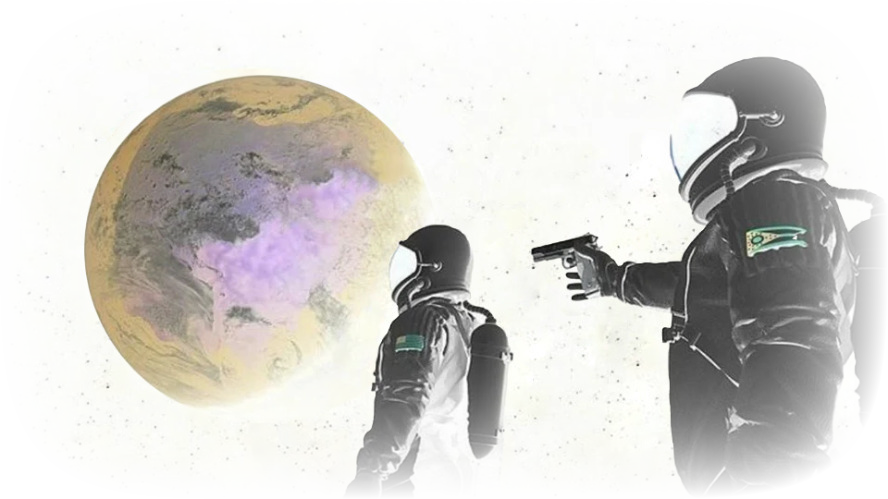
\includegraphics[width=\textwidth]{chapters/superconductivity/from bcs to conventional superconductors/pictures/always.png}
	};
	\node[anchor=center] (a) at (0,0.8) {$(\mathrm{a})$};
	\node[anchor=center] (a) at (3.8,3) {$(\mathrm{b})$};
\end{tikzpicture}
	\caption[$(\mathrm{a})$ Wait, is it a superconductor?; $(\mathrm{b})$ Always has been.]
	{\tabular[t]{@{}l@{}}$(\mathrm{a})$ Wait, is it a superconductor? \\ $(\mathrm{b})$ Always has been.\endtabular}
	\label{fig:always}
\end{figure}
    %
    \printbibliography\nocite{*}
	%
\end{document}